\documentclass{beamer}

%TODO: insert logos in title page, order:
%1. CEA
%2. CRIStAL
%3. Telecom Lille
%4. ARIA
%TODO: transitions with "transparent unseen content"




\usepackage[utf8]{inputenc}
\usepackage[frenchb]{babel}
\usepackage{verbatim}
\usepackage{graphicx}
	\graphicspath{{figures/}{figures/beaune_rejet/}{figures/opera_rejet/}{figures/beaune_varobs/}}
\usepackage{caption}
\usepackage{subcaption}
\usepackage{color}
\usepackage{amsmath}
\usepackage{amsfonts}
\usepackage{mathtools}
\usepackage{bm}
\usepackage{tikz}
	\usetikzlibrary{shapes,arrows}
\usepackage{gensymb}
\usepackage{animate}







\usetheme{boxes}
\usefonttheme[onlymath]{serif}
\usecolortheme{whale}
\beamertemplatenavigationsymbolsempty
\setbeamertemplate{title page}[default][colsep=-4bp,rounded=true]
\setbeamertemplate{sections/subsections in toc}[circle]
\setbeamertemplate{footline}[frame number]
\setbeamertemplate{itemize items}[circle]
\setbeamertemplate{itemize subitem}[square]
\setbeamertemplate{blocks}[rounded][shadow=false]
\setbeamercolor{block title}{bg=blue!40!black,fg=white}
\setbeamercolor{block body}{bg=blue!10,fg=black}

\newtheorem{important}{Important}
\newenvironment<>{important}[1][]{%
	\setbeamercolor{block title}{fg=white,bg=red!40!black}%
	\setbeamercolor{block body}{fg=black,bg=gray!10}
	\setbeamertemplate{itemize item}{\color{red!40!black}$\blacktriangleright$}
	\begin{block}{#2}\textbf{#1}}{\end{block}}

\newenvironment<>{redblock}[1]{%
	\setbeamercolor{block title}{fg=white,bg=red!40!black}%
	\setbeamercolor{block body}{fg=black,bg=red!10}
	\setbeamertemplate{itemize item}{\color{red!40!black}$\blacktriangleright$}
	\begin{block}#2{\small \textbf{#1}}}{\end{block}}

\newenvironment<>{blueblock}[1]{%
	\setbeamercolor{block title}{fg=white,bg=blue!40!black}%
	\setbeamercolor{block body}{fg=black,bg=blue!10}
	\setbeamertemplate{itemize item}{\color{blue!40!black}$\blacktriangleright$}
	\begin{block}#2{\small \textbf{#1}}}{\end{block}}

\newenvironment<>{greenblock}[1]{%
	\setbeamercolor{block title}{fg=white,bg=green!40!black}%
	\setbeamercolor{block body}{fg=black,bg=green!10}
	\setbeamertemplate{itemize item}{\color{green!40!black}$\blacktriangleright$}
	\setbeamercolor{enumerate item}{fg=black}
	\begin{block}#2{\small \textbf{#1}}}{\end{block}}


\newtheorem{algorithme}{Algorithme}
\newenvironment<>{algorithme}[1][]{%
	\setbeamercolor{block title}{fg=white,bg=green!40!black}%
	\setbeamercolor{block body}{fg=black,bg=green!10}
	\setbeamertemplate{itemize item}{\color{green!40!black}$\blacktriangleright$}
	\setbeamercolor{enumerate item}{fg=black}
	\begin{block}{#2}\textbf{#1}}{\end{block}}



\newcommand{\VecQSource}{{\bm{q}}}
\newcommand{\VecPosSource}{{\bm{x_s}}}
\newcommand{\VecTheta}{{\bm{\theta}}}
\newcommand{\VecObs}{{\bm{\eta}}}
\newcommand{\MatC}{{\bm{C}}}
\newcommand{\VecErreur}{{\bm{\varepsilon}}}
\newcommand{\MatSigma}{{\bm{\Sigma}}}
\newcommand{\MatI}{{\bm{I}}}
\newcommand{\VecMeanQ}{{\bm{\mu}_q}}
\newcommand{\MatCovQ}{{\bm{\Sigma}_q}}
\newcommand{\PostMeanQ}{{\widetilde{\bm{\mu}}_q}}
\newcommand{\PostCovQ}{{\widetilde{\bm{\Sigma}}_q}}
\newcommand{\VecMu}{{\bm{\mu}}}



\definecolor{lightgreen}{rgb}{0.0,0.8,0.0}
\definecolor{lightblue}{rgb}{0.3,0.8,1.0}
\definecolor{lightred}{rgb}{0.874,0.180,0.105}
\definecolor{gray}{rgb}{0.4,0.4,0.4}
\definecolor{lightgray}{rgb}{0.8,0.8,0.8}
\definecolor{shadecolor}{rgb}{0.9,0.9,0.9}




\title{Inférence bayésienne adaptative pour la reconstruction de source en dispersion atmosphérique}
\author{Harizo RAJAONA}
\institute{Directeur de thèse: François SEPTIER}
% logo of my university
\titlegraphic{
	\centering
	
\includegraphics[width=0.65\textwidth]{logos_big}
}
\date{21 novembre 2016}

\begin{document}
	
	
	
	
\AtBeginSection[]
{
	\begin{frame}
		\tableofcontents[currentsection]
		% Die Option [pausesections]
	\end{frame}
}
	
	
\begin{frame}
	\titlepage
\end{frame}
\begin{frame}
	\tableofcontents
\end{frame}

\section{Contexte et problématique}

% ===== Contexte (1) ================================================================
\begin{frame}
	\frametitle{Contexte}
	Les rejets \textbf{NRBC}\footnote{\textbf{N}ucléaires, \textbf{R}adiologiques, \textbf{B}iologiques, \textbf{C}himiques} dans l'atmosphère peuvent être d'origine:
	\begin{itemize}
		\item accidentelle (fuite ou explosion sur un site industriel),
		\item malveillante (actes terroristes)
	\end{itemize}
	\begin{figure}
		\centering
		\begin{subfigure}[b]{0.33\textwidth}
			\centering
			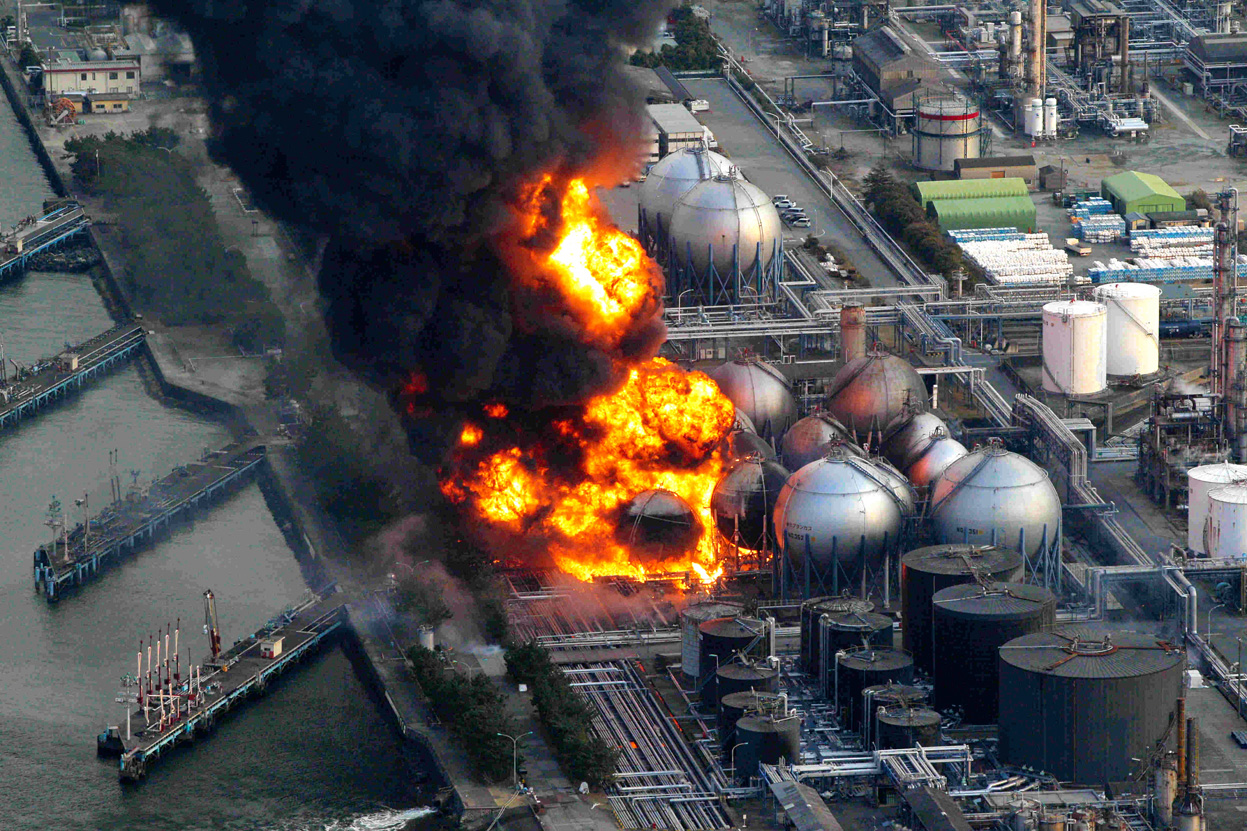
\includegraphics[width=\textwidth]{fukushima}
			\caption*{Fukushima (2011)}
		\end{subfigure}
		\hfill
		\begin{subfigure}[b]{0.3\textwidth}
			\centering
			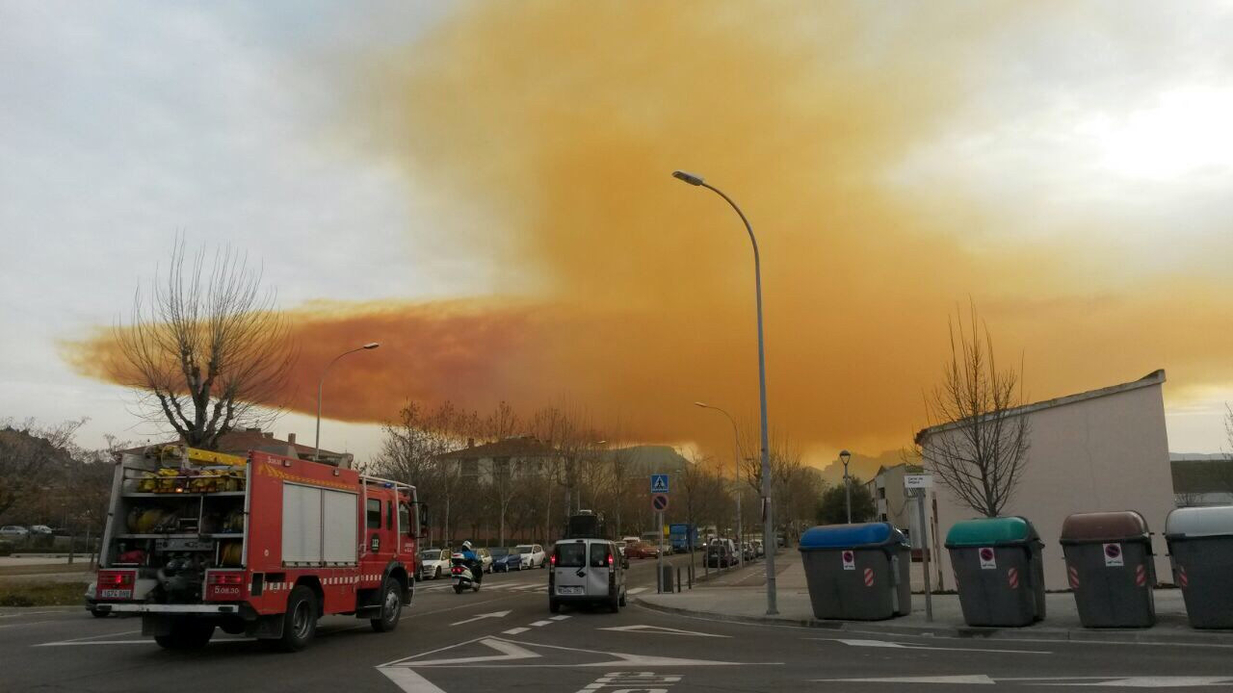
\includegraphics[width=\textwidth]{igualada}
			\caption*{Igualada (2015)}
		\end{subfigure}
		\hfill
		\begin{subfigure}[b]{0.3\textwidth}
			\centering
			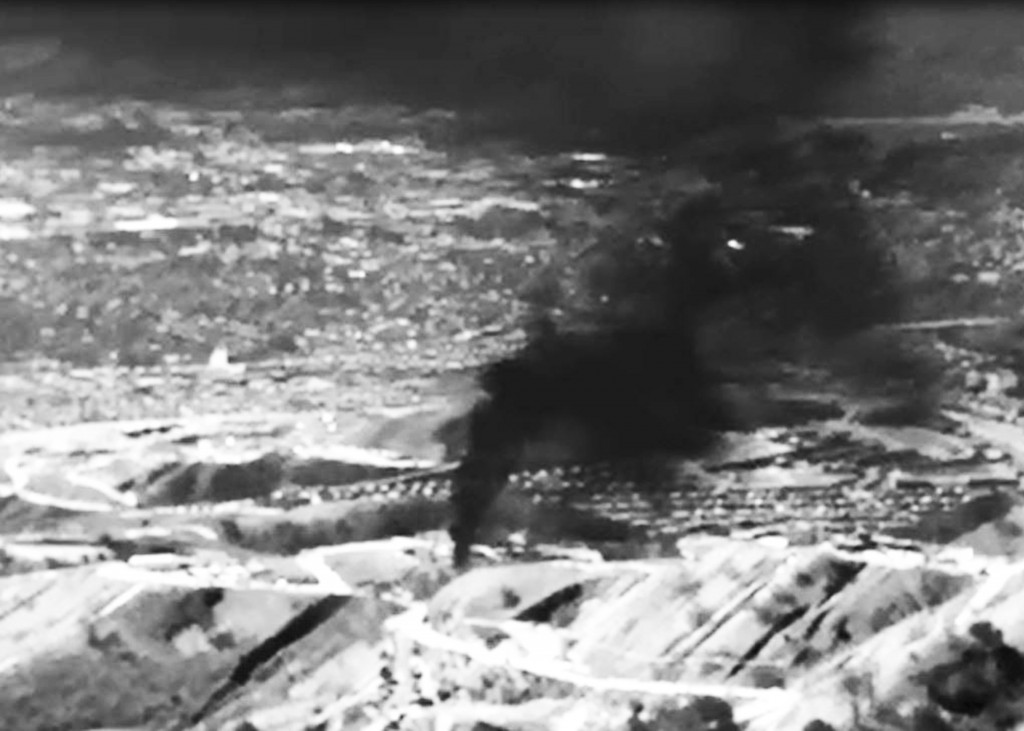
\includegraphics[width=\textwidth]{los_angeles}
			\caption*{Los Angeles (2015)}
		\end{subfigure}
	\end{figure}
	
	Priorités:
	\begin{itemize}
		\item informer et protéger les populations,
		\item atténuer/neutraliser le risque.
	\end{itemize}
\end{frame}

% ===== Contexte (2) ================================================================

\begin{frame}
	\frametitle{Contexte}
	Outils de détection et d'évaluation du risque:
	\begin{itemize}
		\item données d'\textbf{observation} (capteurs mesurant la concentration de polluant)
		\item outils de \textbf{modélisation} des phénomènes atmosphériques
	\end{itemize}
	\begin{figure}
		\centering

				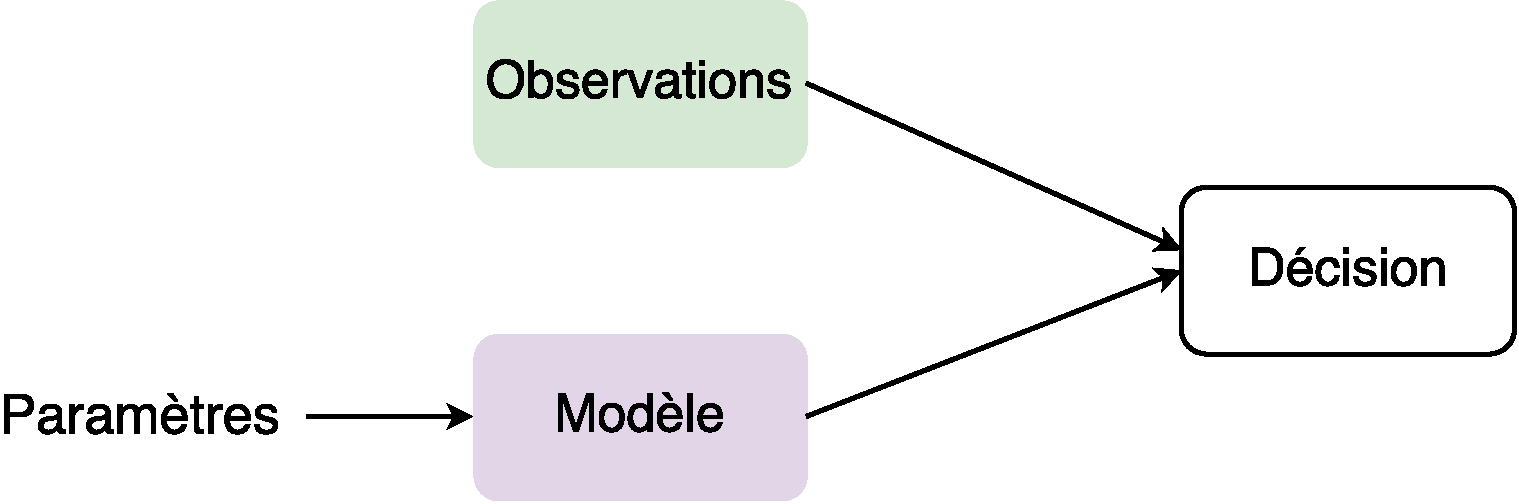
\includegraphics[width=0.9\textwidth]{diagram_context_step_2.pdf}
		
	\end{figure}
\end{frame}

% ===== Physique de l'atmosphère ================================================================

\begin{frame}
	\frametitle{Dispersion atmosphérique}
	\begin{blueblock}{Modèle de dispersion}
		Outil de calcul numérique permettant, grâce à la résolution d'une équation d'advection-diffusion, de simuler la propagation dans l'atmosphère d'un rejet de polluant.
	\end{blueblock}
	
	
	Typologie des modèles selon:
	\begin{itemize}
		\item  l'échelle (locale, régionale, synoptique),
		\item le degré de simplification des équations de la mécanique des fluides
	\end{itemize}
	
	Paramètres d'entrée:
	\begin{itemize}
		\item données météorologiques: vent (direction + vitesse), température, humidité, nébulosité, flux de rayonnement...
		\item \textbf{terme source}: position, quantités émises, durée, substance émise...
	\end{itemize}
\end{frame}

% =====  Terme source  ================================================================
\begin{frame}
	\frametitle{Terme source: définitions}
	Hypothèses sur la nature de la source:
	\begin{itemize}
		\item \textbf{localisée} (représentée par un point géographique $\VecPosSource \in \mathbb{R}^3$),
		\item \textbf{unique} (un seul point d'émission),
		\item \textbf{non-instantanée}, avec un profil temporel d'émission: $$\VecQSource = \left(q(t'_1), q(t'_2), \cdots, q(t'_{T_s})\right)$$
	\end{itemize}
%	 vecteur $\VecQSource \in \mathbb{R}^{T_s} $:
	\begin{columns}
		\column{0.75\linewidth}
			\begin{figure}
				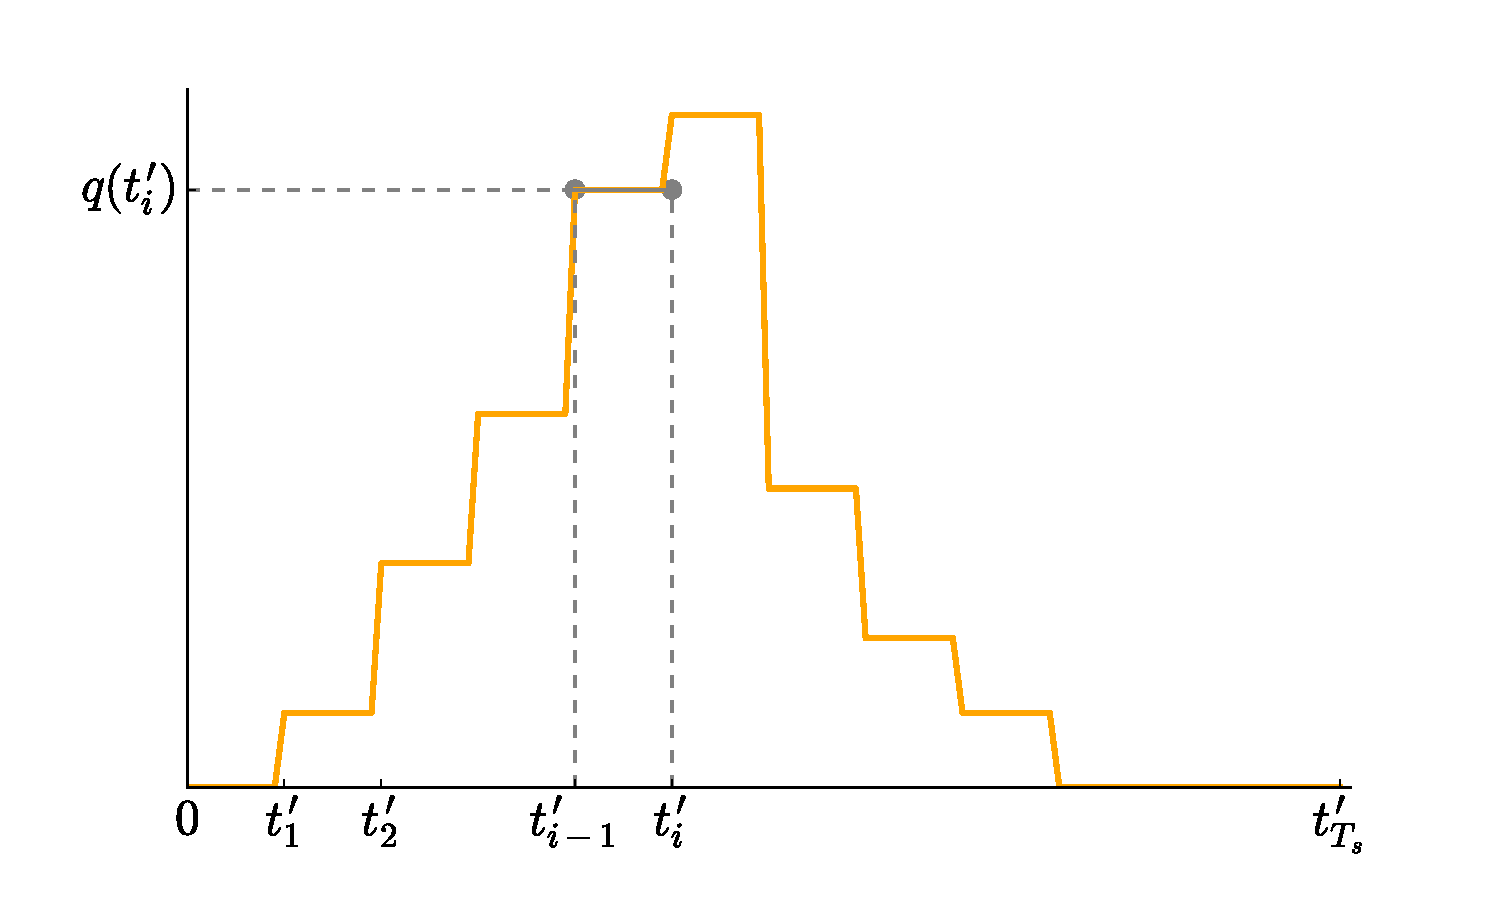
\includegraphics[width=0.99\textwidth]{courbe_profil_source_paliers}
			\end{figure}
		\column{0.25\linewidth}
		{$\Rightarrow$ \small émission constante sur le palier $ [t'_{i-1}, t'_i] $}
	\end{columns}

	
\end{frame}

% =====  Terme source  ================================================================

\begin{frame}
	\frametitle{Terme source: estimation (principe)}
	Reconstruire les paramètres d'un terme source (STE\footnote{\textit{\textbf{S}ource \textbf{T}erm \textbf{E}stimation}}) à partir des observations est un problème inverse.
	
	\begin{figure}
		\centering
		
\includegraphics[width=0.75\textwidth]{modele_direct} \\
		\vspace{0.5cm}
		
\includegraphics[width=0.75\textwidth]{modele_inverse}
	\end{figure}

\end{frame}

\begin{frame}
	\frametitle{Terme source: estimation (état de l'art)}
		
		Approches existantes: 
		\begin{itemize}
			\item \textbf{rétro-transport}: étude de la forme duale des équations d'advection-diffusion 
			\begin{itemize}
				\item solution intuitive du problème physique
				\item {\color{lightred}requiert un modèle rétrograde fiable}
			\end{itemize}
			\item \textbf{formulation linéaire du problème inverse}: minimisation d'une fonction-coût (éventuellement régularisée) sur un espace maillé dans le temps et l'espace
			\begin{itemize}
				\item implémentation simple 
				\item {\color{lightred}dimension élevée, choix du maillage}
			\end{itemize}
			\item \textbf{algorithmes évolutionnaires}: sélection, croisements et mutations sur une population d'individus
			\begin{itemize}
				\item résolution de problèmes à forte complexité combinatoire
				\item {\color{lightred}temps de calcul élevés, réglage des paramètres}
			\end{itemize}
			\item \textbf{ méthodes bayésiennes et simulation stochastique}: calcul d'une loi de probabilité a posteriori par échantillonnage
		\end{itemize}
\end{frame}


% =====  Problématique de recherche ================================================================

\begin{frame}
	\frametitle{Problématique de recherche}
	On se concentre sur les \textbf{méthodes bayésiennes}:
	\begin{itemize}
		\item approche probabiliste permettant de \textbf{quantifier les incertitudes},
		\item exploitation d'un nombre limité de mesures (\textbf{régularisation}),
		\item {\color{red} temps de calcul potentiellement élevés,}
		\item {\color{red} estimation disjointe de la position et du profil d'émission.}
	\end{itemize}
	
    \begin{redblock}{Problématique}
    	\begin{itemize}
    		\item Développer une méthode bayésienne pour estimer la localisation \textbf{et} le profil d'émission d'une source.
    		\item Coupler cette méthode avec un modèle de dispersion atmosphérique dans une chaîne de calcul opérationnelle.
    	\end{itemize}
    \end{redblock}
\end{frame}
% ++++++++++++++++++++++++++++++++++++++++++++++++++++++++++++++++++++++++
% ++++++++++++++++++++++++++++++++++++++++++++++++++++++++++++++++++++++++
\section{Méthodologie adaptative pour l'inférence bayésienne}
% =====  Le choix bayésien ================================================================

\begin{frame}
	\frametitle{Inférence bayésienne}
	\textbf{Principe}: estimation probabiliste des paramètres $\VecTheta$ d'un système ayant généré un ensemble d'observations $\VecObs$.
	\begin{itemize}
		\item $\VecTheta ~\Rightarrow$ paramètres du terme source
		\item $\VecObs ~ \Rightarrow$ mesures de concentration observées
	\end{itemize}
	\begin{blueblock}{Règle de Bayes}
		$$ \pi(\VecTheta) = p(\VecTheta | \VecObs) = \dfrac{p(\VecTheta)p(\VecObs|\VecTheta)}{p(\VecObs)} \propto p(\VecTheta)p(\VecObs|\VecTheta) $$
		\begin{itemize}
			\item loi \textbf{a posteriori} $\pi(\VecTheta)$: information sur $\VecTheta$ connaissant $\VecObs$,
			\item loi\textbf{ a priori }$p(\VecTheta)$: information préalable sur $\VecTheta$,
			\item \textbf{vraisemblance} $p(\VecObs | \VecTheta)$: probabilité d'observer $\VecObs$ pour $\VecTheta$ fixé.
		\end{itemize}
		\end{blueblock}
\end{frame}
% =====  Méthodes MC  ================================================================

\begin{frame}
	\frametitle{Inférence bayésienne}
	\begin{itemize}
	\item \textbf{Problème}: {\color{red} impossible d'obtenir une expression analytique pour $\pi(\VecTheta)$ ! } \\
	
	 $\Rightarrow$ recours à des méthodes d'approximation numérique
	
	\begin{blueblock}{Méthodes de Monte-Carlo}
		Permettent d'approximer l'espérance de toute fonction d'une variable aléatoire  de loi $\pi$ en échantillonnant sur cette loi:
%		\begin{equation*}
%			\begin{split}
%				\mathbb{E}_{\pi}[\psi(\VecTheta)] &= \int \psi(\VecTheta)\pi(\VecTheta)d\VecTheta \\
%				& \simeq \dfrac{1}{N} \sum\limits_{i=1}^{N}\psi(\theta^{(i)}), ~ ~ ~ \theta^{(i)} \sim \pi
%			\end{split}
%		\end{equation*}
		$$ \mathbb{E}_{\pi}[f(\VecTheta)] = \int f(\VecTheta)\pi(\VecTheta)d\VecTheta \simeq \dfrac{1}{N} \sum\limits_{i=1}^{N}f(\theta^{(i)}), ~ ~ ~ \theta^{(i)} \sim \pi $$
	\end{blueblock}
	
	\item Obtention d'estimateurs bayésiens par simulation (ex: poser $f(\VecTheta) = \VecTheta$ pour le MMSE\footnote{\textit{\textbf{M}inimum \textbf{M}ean \textbf{S}quare \textbf{E}stimator}}).
	
	\end{itemize}
\end{frame}

\begin{frame}
	\frametitle{Méthodes d'échantillonnage}
%	Plusieurs méthodes permettent d'échantillonner depuis la loi cible:
	\begin{itemize}
		\item Algorithmes \textbf{MCMC}\footnote{\textit{\textbf{M}arkov \textbf{C}hain \textbf{M}onte \textbf{C}arlo}}: $\pi$ est la distribution stationnaire d'une chaîne de Markov construite par itérations successives.
		\begin{itemize}
			\item Metropolis-Hastings
			\item échantillonneur de Gibbs
		\end{itemize}
		Bons résultats obtenus dans la littérature STE:
		\begin{itemize}

			\item en milieu urbain: Keats (2007), Chow (2008)
			\item en multi-source: Yee (2008)
		\end{itemize}
		
		Inconvénients:
		\begin{itemize}
			\item perte d'une partie des échantillons générés (\textit{burn-in})
			\item états corrélés (non-parallélisable)
			\item MH: performances liées au choix du noyau et de l'initialisation
			\item Gibbs: requiert les lois conditionnelles de $\VecTheta$
		\end{itemize}
		
		\item Algorithmes \textbf{d'échantillonnage d'importance} (\textbf{IS}\footnote{\textit{\textbf{I}mportance \textbf{S}ampling}}): tirage d'une population d'échantillons pondérés (ou particules) à partir d'une loi de proposition.
	\end{itemize}
\end{frame}

% =====  MCMC (1)  ================================================================

%\begin{frame}
%	\frametitle{MCMC}
%	\begin{block}{Markov Chain Monte-Carlo (MCMC)}
%		Méthodes de construction d'une chaîne de Markov dont la distribution stationnaire est la loi cible $\pi$.
%	\end{block}
%	
%	Approches classiques:
%	\begin{itemize}
%		\item algorithme de Metropolis-Hastings
%		\item échantillonneur de Gibbs
%	\end{itemize}
%	
%    \begin{algorithme}[Exemple: Metropolis-Hastings (MH)\\]
%	    Initialiser la chaîne à $\VecTheta^{(0)}$ et choisir un noyau de transition $\mathcal{K}(\cdot, \cdot)$. A la i-ème itération et jusqu'à convergence:\\
%	    \begin{enumerate}
%	    	\item Tirer $\VecTheta^* \sim \mathcal{K}(\VecTheta^{(i-1)},\VecTheta^*)$
%	    	\item Calculer $r = \text{min }\left\{1, \dfrac{\pi(\VecTheta^*)\mathcal{K}(\VecTheta^*,\VecTheta^{(i-1)})}{\pi(\VecTheta^{(i-1)})\mathcal{K}(\VecTheta^{(i-1)},\VecTheta)}\right\}$
%	    	\item Accepter $\VecTheta^{(i)} = \VecTheta$ avec la probabilité $r$. Si rejet, garder $\VecTheta^{(i)} = \VecTheta^{(i-1)}$	    	
%	    \end{enumerate}
%    \end{algorithme}
%	
%\end{frame}

% =====  MCMC (2)  ================================================================
%\begin{frame}
%	\frametitle{MCMC}
%	MH sur un mélange de gaussiennes: {\small $\pi(\VecTheta) = \gamma\mathcal{N}(\VecTheta|\mu_1, \sigma_1^2) + (1-\gamma)\mathcal{N}(\VecTheta | \mu_2, \sigma_2^2)$}
%	\begin{columns}
%		\column{0.8\linewidth}
%			\begin{figure}
%				\only<1>{
%				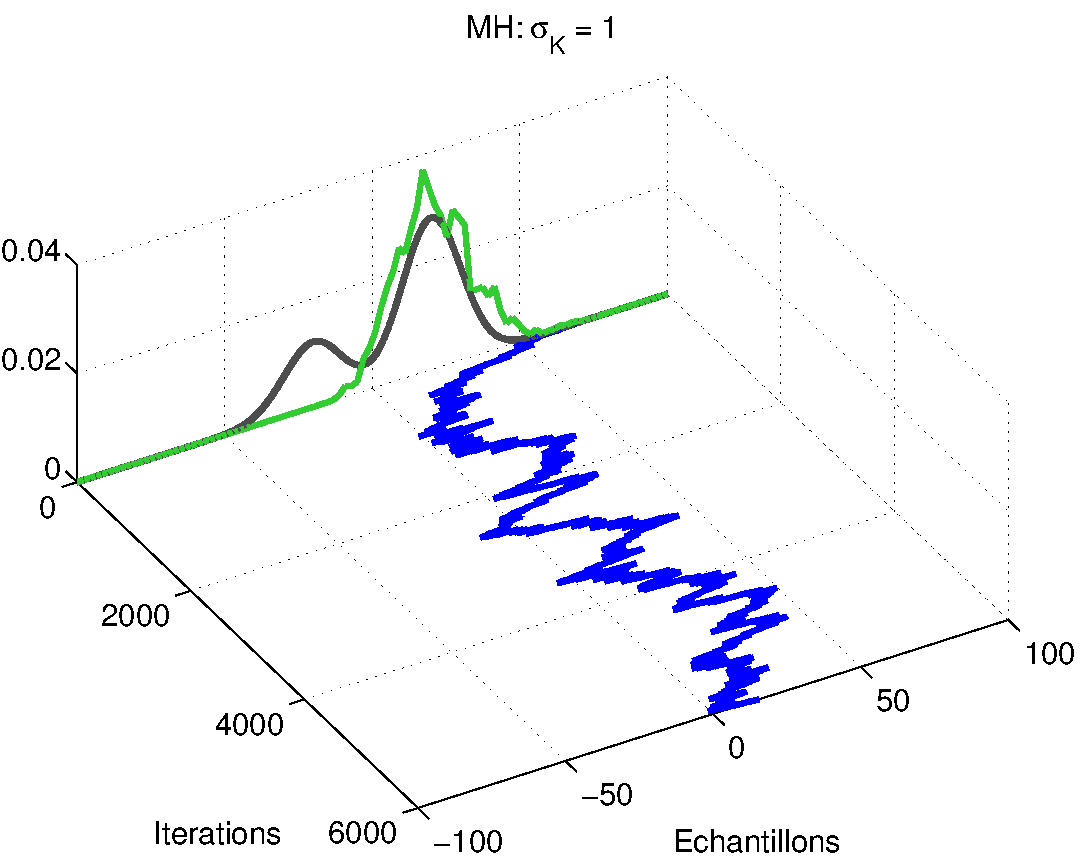
\includegraphics[width=0.75\textwidth]{mh_1}
%				}
%				\only<2>{
%					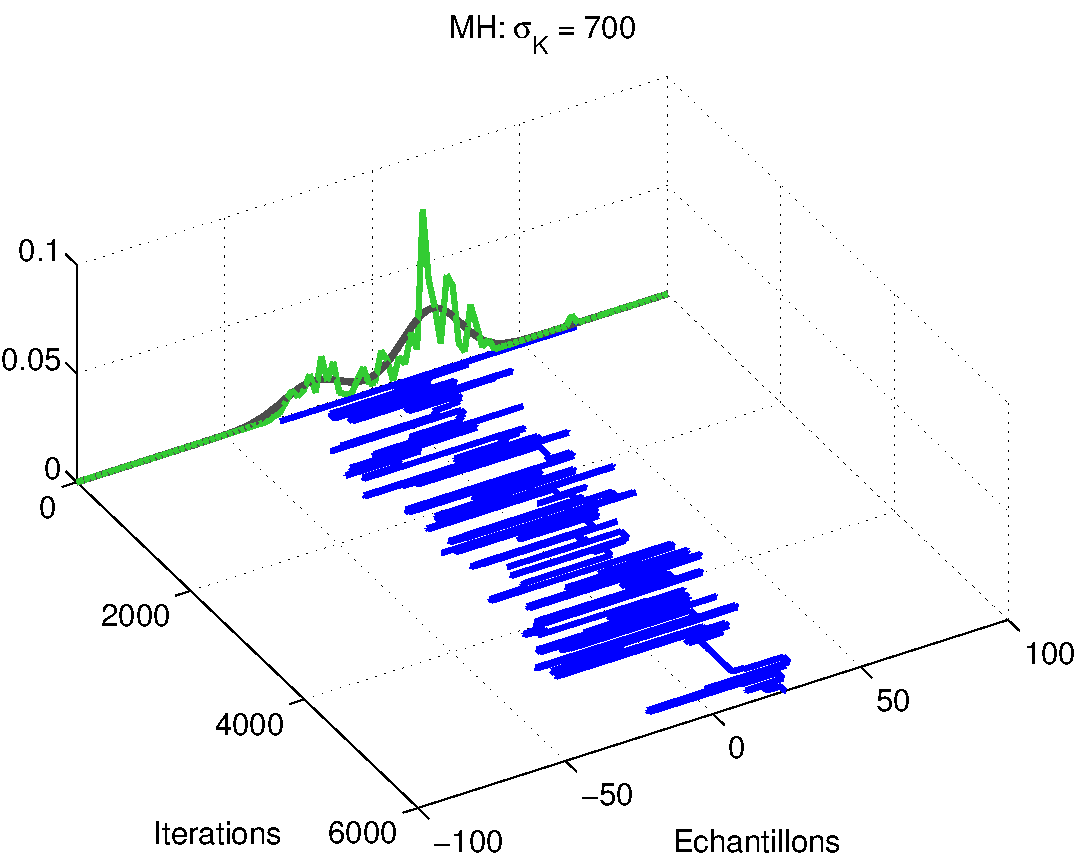
\includegraphics[width=0.75\textwidth]{mh_2}
%				}
%				\only<3>{
%					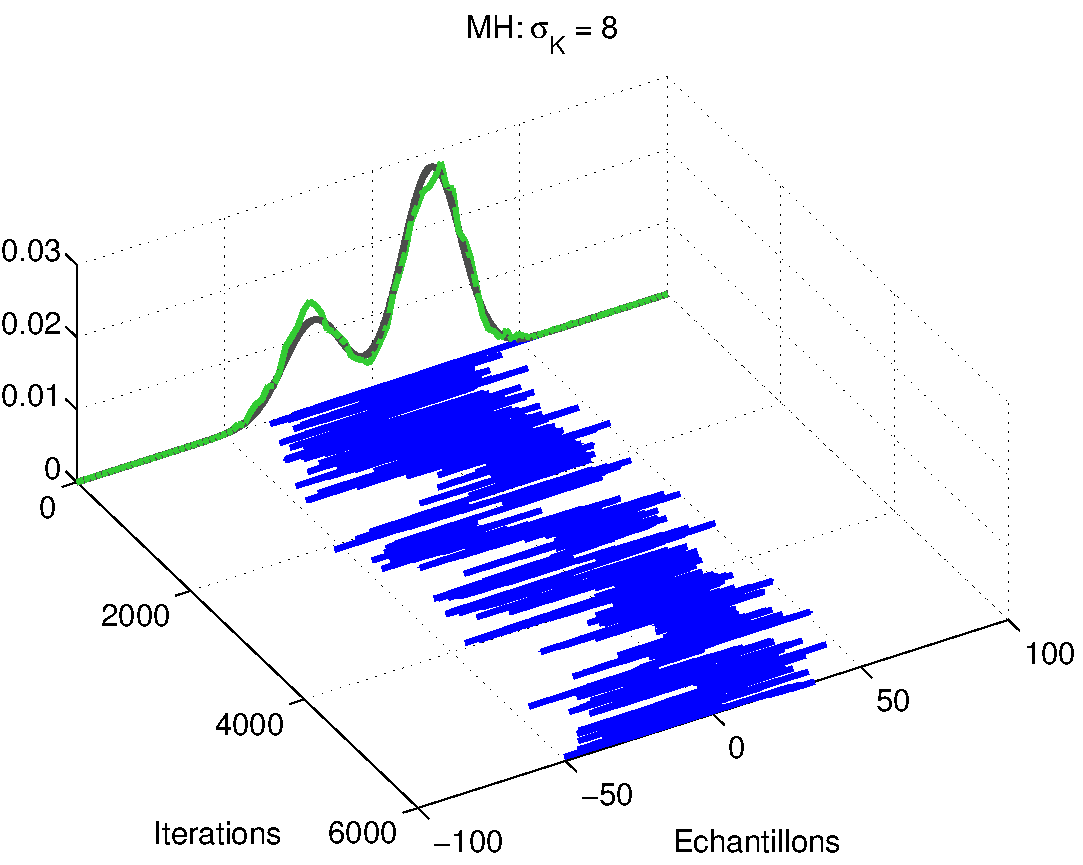
\includegraphics[width=0.75\textwidth]{mh_3}
%				}
%			\end{figure}
%		\column{0.2\linewidth}
%{\small 			$\gamma = 0.3$\\
%			$\mu_1 = -20$\\
%			$\sigma_1 = 10$\\
%			$\mu_2 = 20$\\
%			$\sigma_2 = 10$\\}
%	\end{columns}
%	\begin{itemize}
%		\item<1>\textit{Bad mixing}: transitions trop {\color{red}faibles}
%		\item<2>\textit{Bad mixing}: transitions trop {\color{red}grandes}
%		\item<3>\textit{Good mixing}
%		\item<3> Performances liées aux choix du noyau et de l'initialisation !
%	\end{itemize}
%\end{frame}

% =====  MCMC (2)  ================================================================
%\begin{frame}
%	\frametitle{MCMC}
%	
%	Limitations de l'approche MCMC:
%	\begin{itemize}
%		\item états consécutifs corrélés: non-parallélisable
%		\item perte d'une partie des échantillons générés (\textit{burn-in})
%		\item MH: performances liées aux choix du noyau et de l'initialisation
%		\item Gibbs: nécessite de connaître les lois conditionnelles de $\VecTheta$
%	\end{itemize}
%	
%	
%\end{frame}

%% =====  IS (1)  ================================================================
%\begin{frame}
%	\frametitle{Echantillonnage d'importance}
%	\begin{block}{Echantillonnage d'importance}
%		\begin{enumerate}
%			\item Définir une loi de proposition $\varphi(\VecTheta)$ à support inclus dans celui de $\pi$
%			\item Tirer $\VecTheta \sim \varphi$
%			\item Calculer les poids d'importance $w(\VecTheta) = \dfrac{\pi(\VecTheta)}{\varphi(\VecTheta)}$
%		\end{enumerate}
%	\end{block}
%	
%	Normalisation nécessaire si $\pi$ connu uniquement à une constante près:
%	$$ \widetilde{w}(\VecTheta) = \dfrac{w^{(i)}(\VecTheta)}{\sum\limits_{i=1}^N w^{(i)}(\VecTheta)} $$
%		
%	On peut alors approximer la loi cible: 
% $$ \pi(\VecTheta) \simeq \sum\limits_{i=1}^N \widetilde{w}(\VecTheta^{(i)})\delta_{\VecTheta^{(i)}}(\VecTheta) $$
%\end{frame}
%% =====  IS (2)  ================================================================
\begin{frame}
	\frametitle{Echantillonnage d'importance}
	\begin{figure}
			\centering
			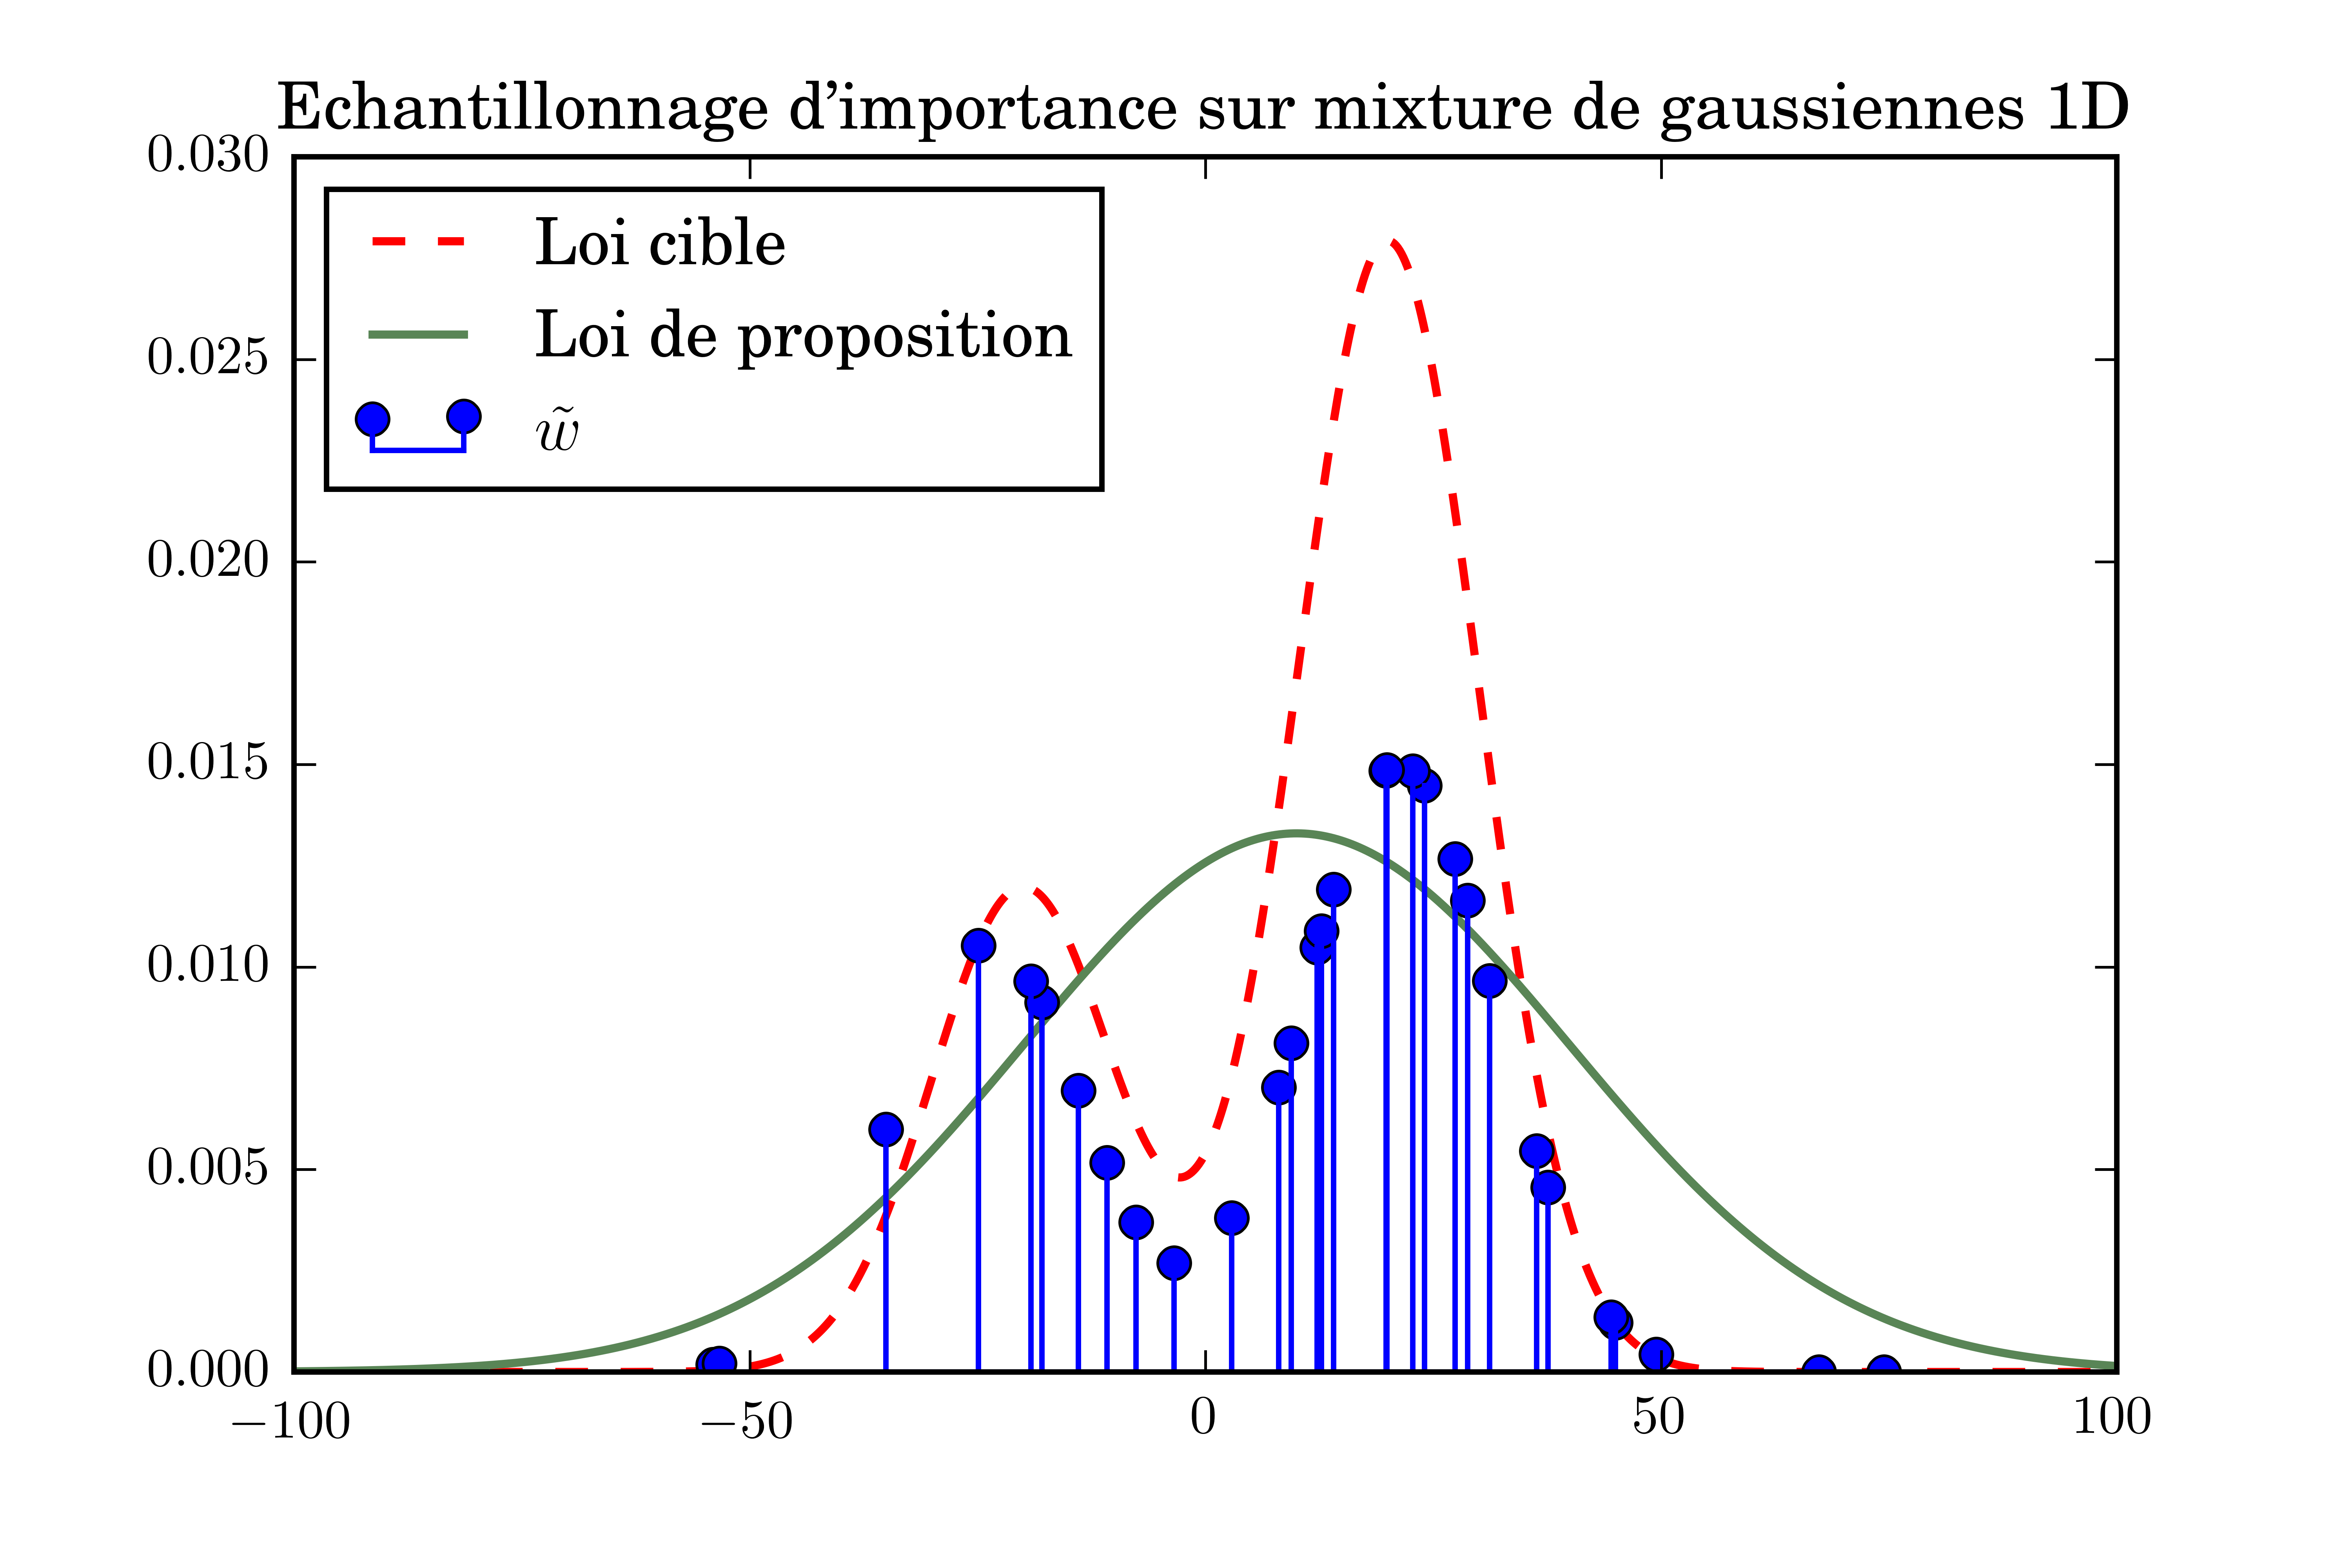
\includegraphics[width=0.8\textwidth]{is_vanilla}
		\end{figure}
{ 		Avantages:
		\begin{itemize}
			\item échantillons i.i.d\footnote{\textbf{i}ndépendants \textbf{i}dentiquement \textbf{d}istribués}.: traitement parallélisable
			\item exploitation de tous les échantillons générés
		\end{itemize}}
\end{frame}

\begin{frame}
	\frametitle{Echantillonnage d'importance}
		Inconvénients:
		\begin{itemize}
			\item {\color{lightred}performances fortement conditionnées par le choix de la loi de proposition !}
		\end{itemize}
		\begin{figure}
			\centering
			\only<1>{
				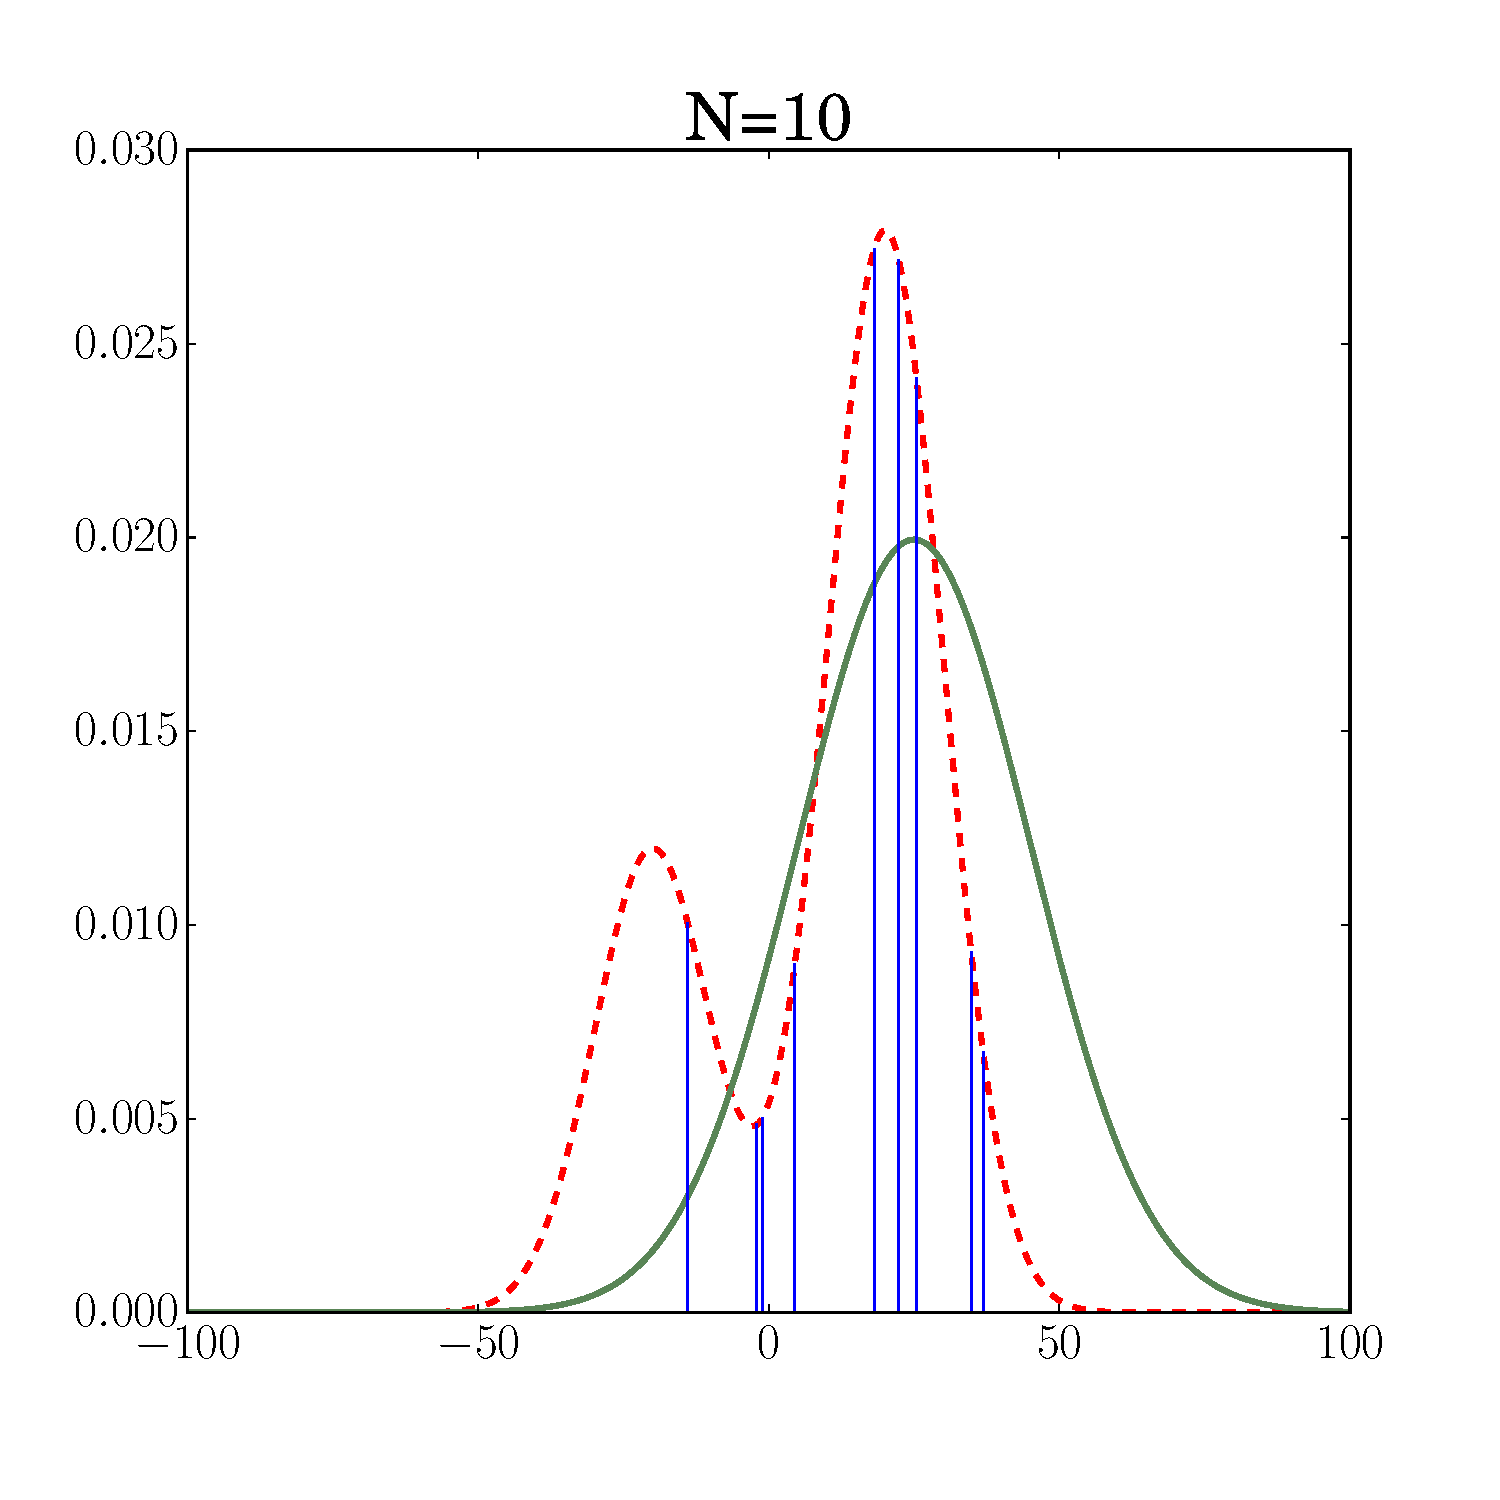
\includegraphics[width=0.6\textwidth]{is_vanilla_bad_10}
				}
			\only<2>{
				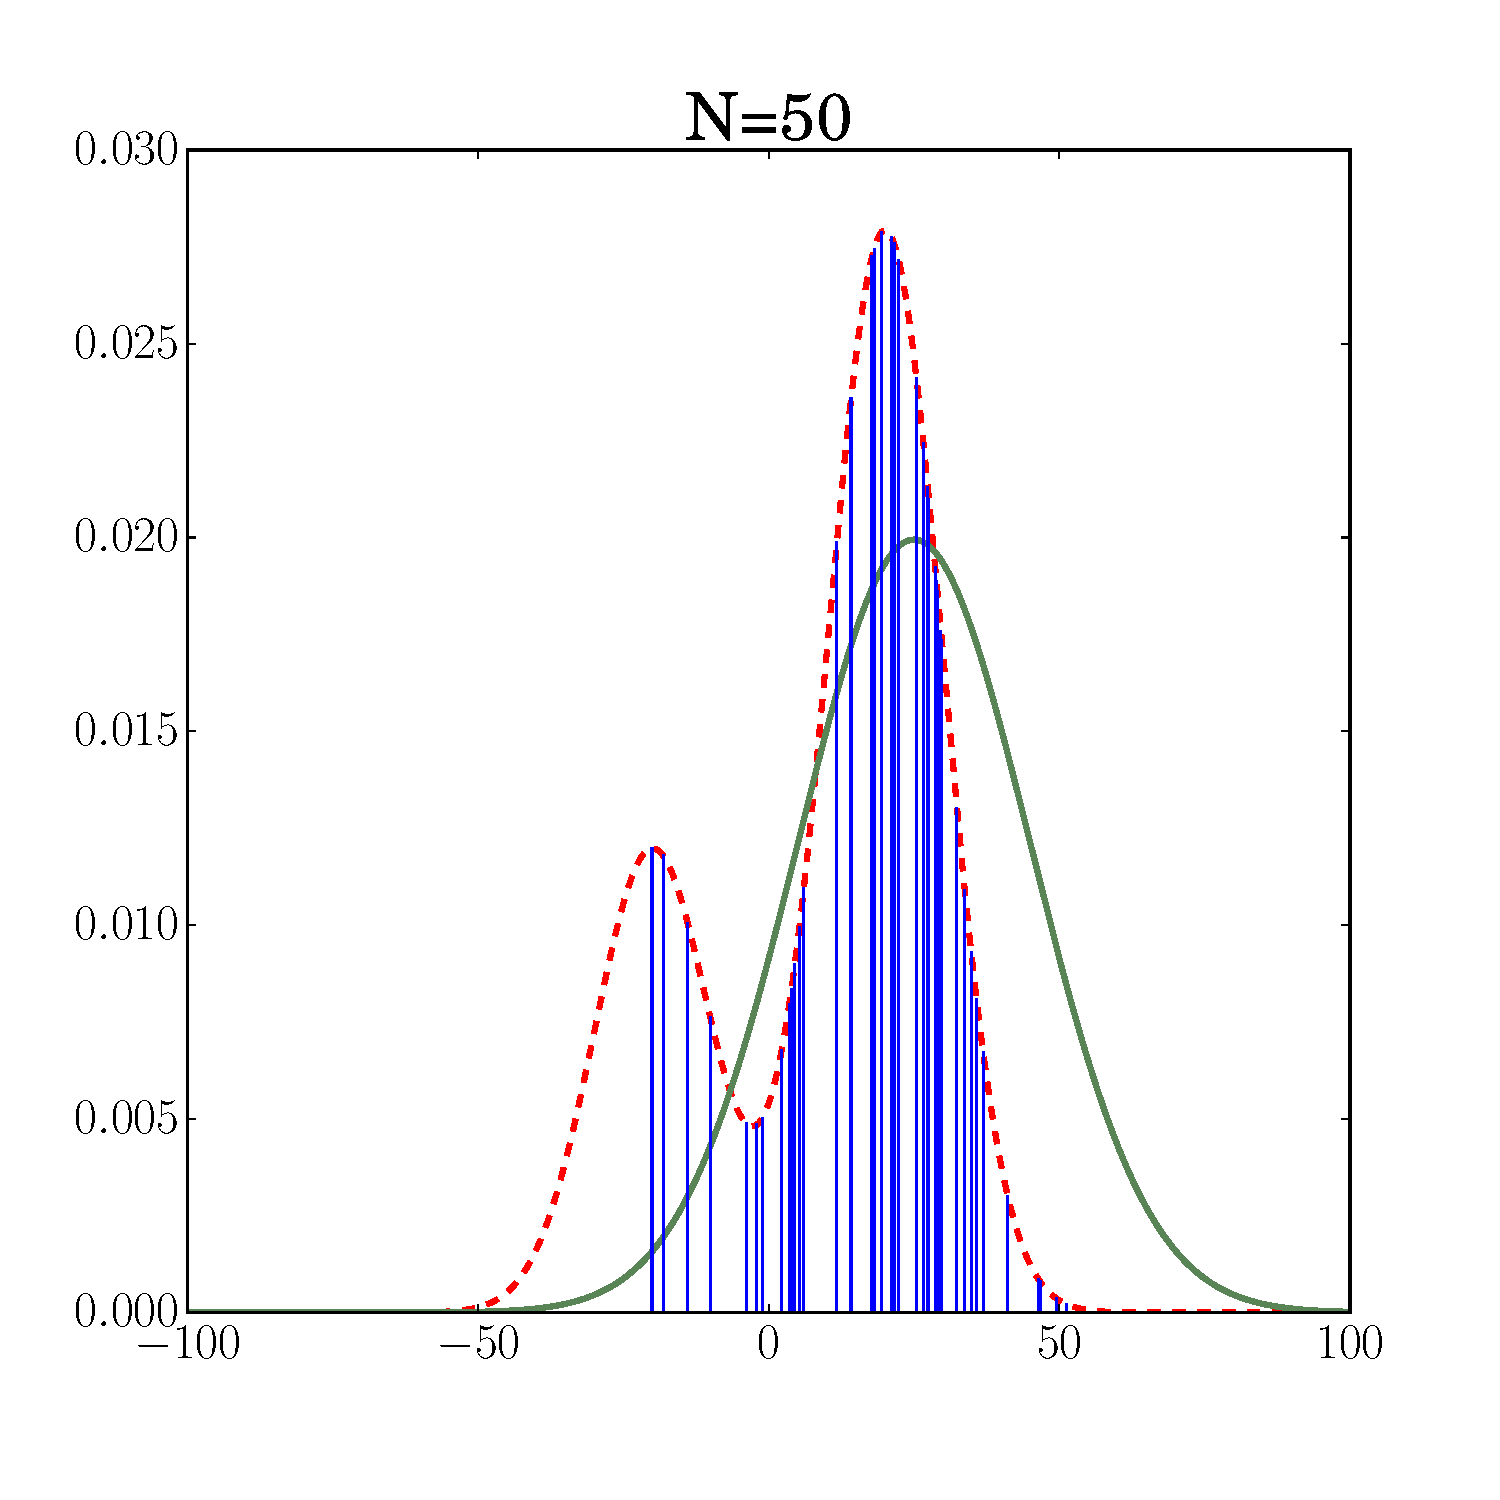
\includegraphics[width=0.6\textwidth]{is_vanilla_bad_50}
			}
			\only<3>{
				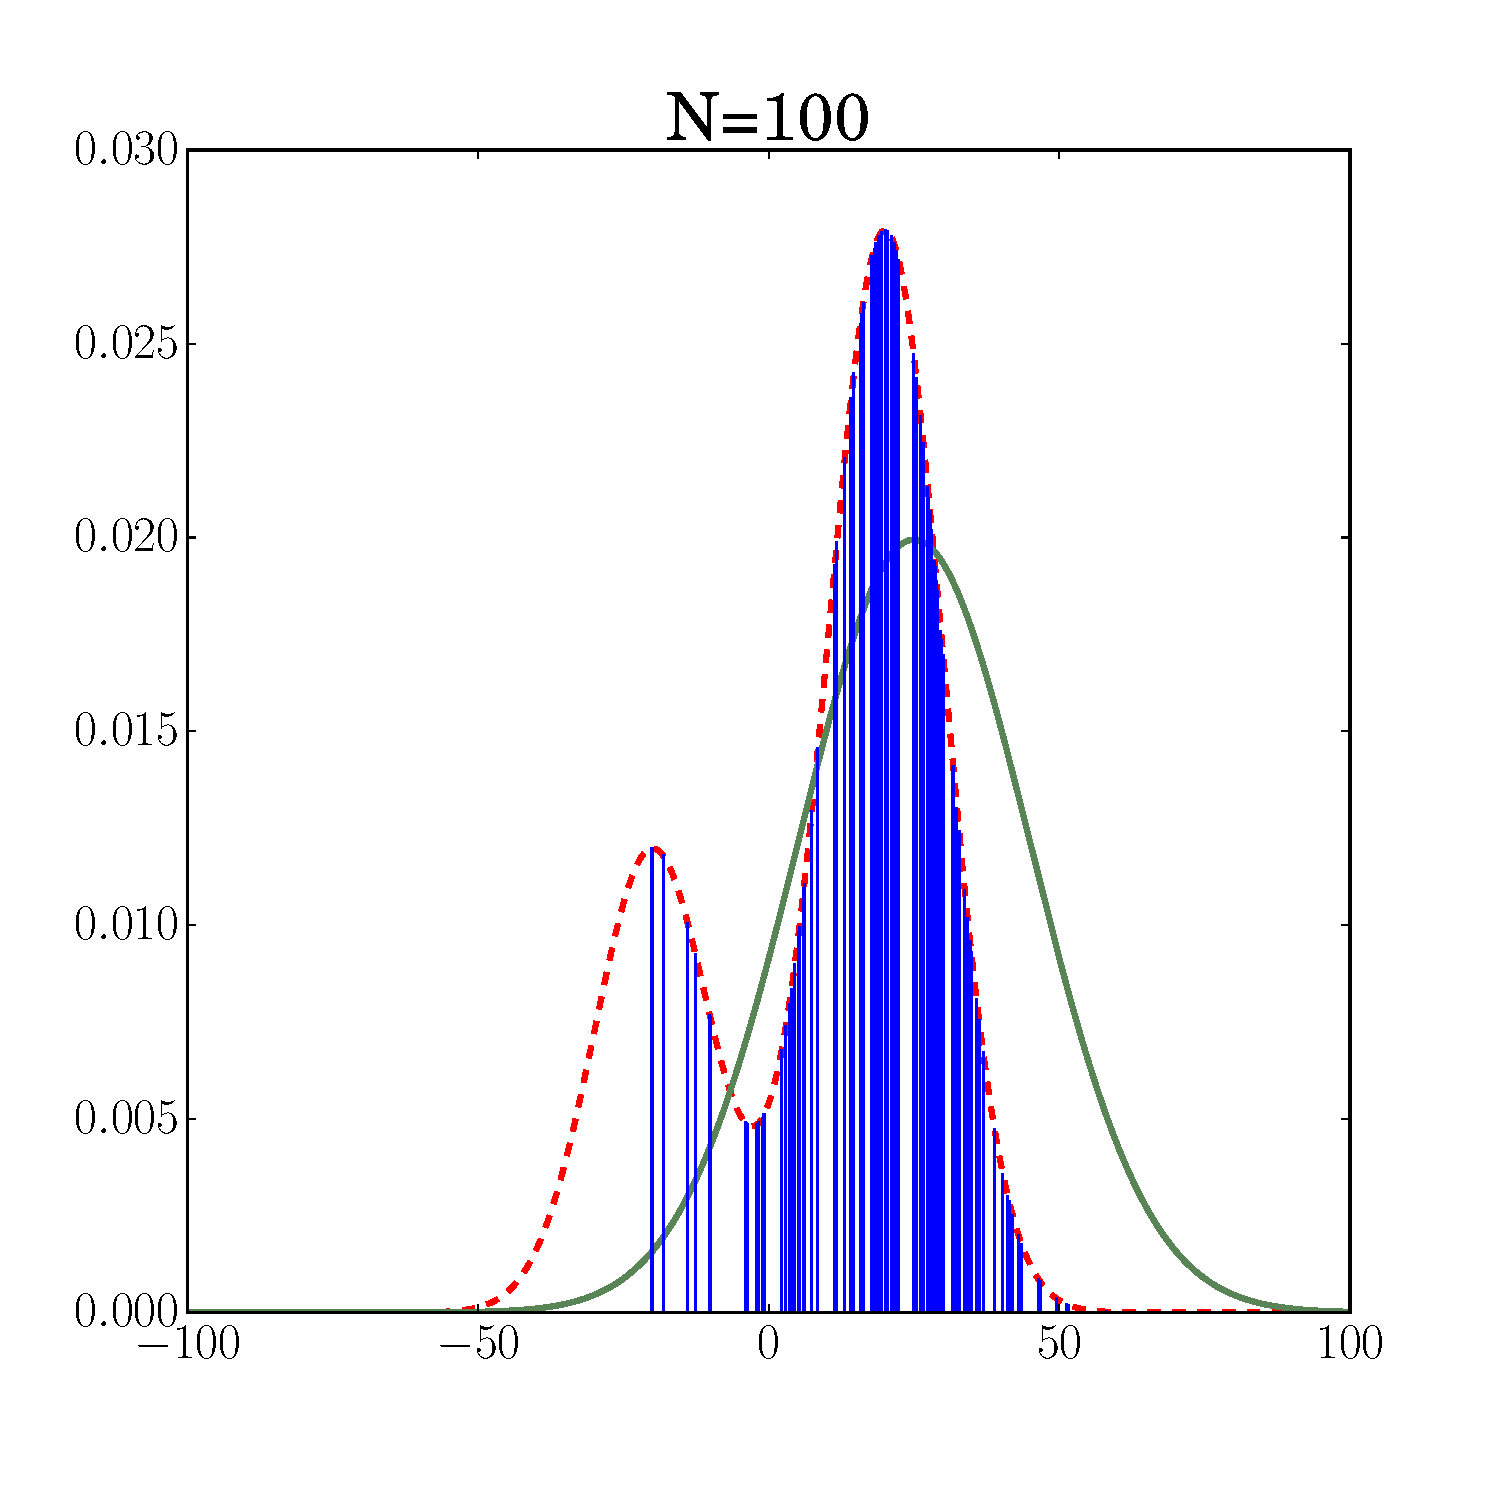
\includegraphics[width=0.6\textwidth]{is_vanilla_bad_100}
			}
			\only<4>{
				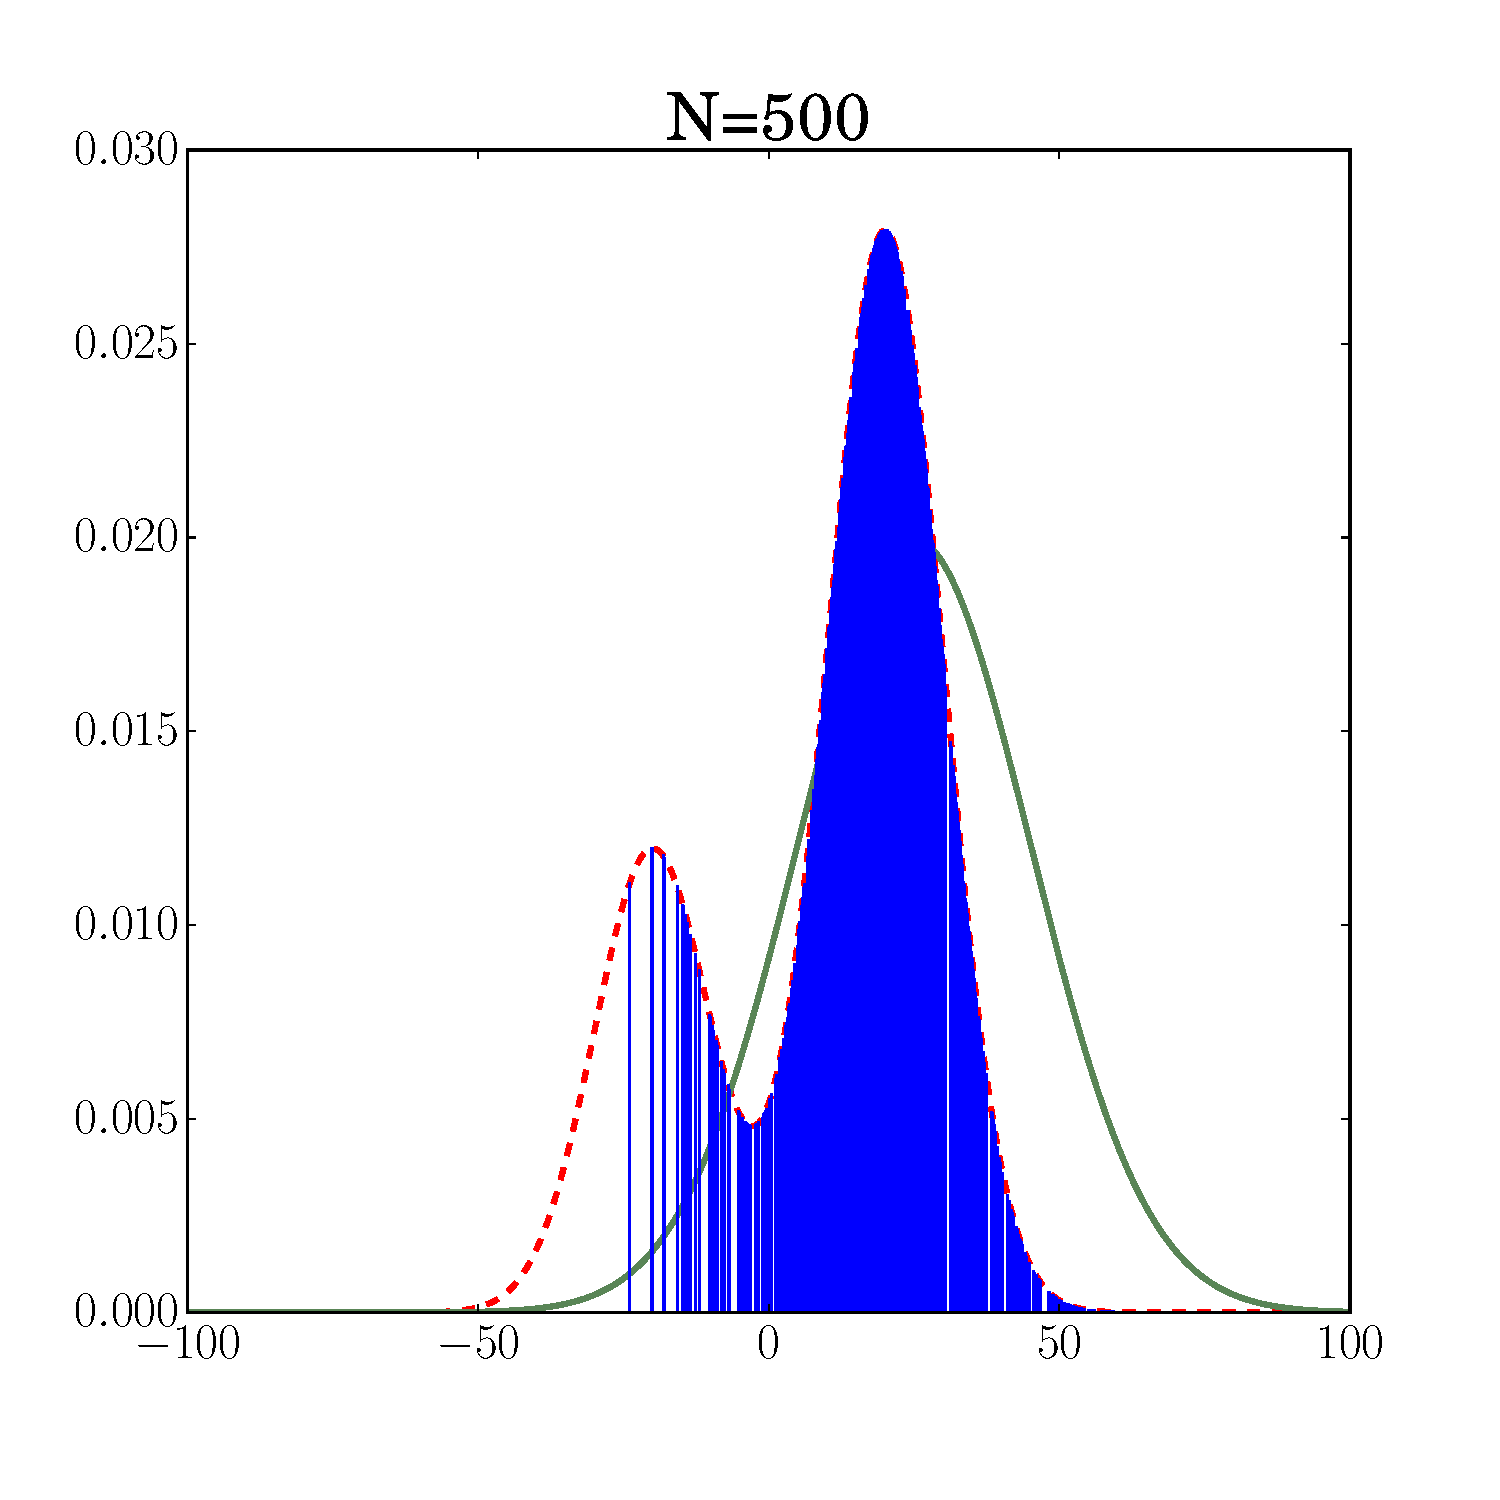
\includegraphics[width=0.6\textwidth]{is_vanilla_bad_500}
			}
		\end{figure}
\end{frame}
%% =====  IS adaptatif  ================================================================
\begin{frame}
	\frametitle{Echantillonnage d'importance adaptatif}
	\textbf{Solution}: adapter itérativement la loi de proposition $\varphi$
	\begin{blueblock}{Population Monte Carlo [Cappé et al., 2004]}
		Introduction du concept d'adaptation par minimisation de : $$ KL(\pi, \varphi) = \int \log \bigg(\dfrac{\pi(\VecTheta)}{\varphi(\VecTheta)}\bigg)\pi(\VecTheta)d\VecTheta ~~~ \text{(divergence KL)} $$
	\end{blueblock}
	
	\begin{blueblock}{D-kernel PMC [Douc et al., 2007]}
		\begin{itemize}
			\item Loi de proposition $\varphi_{\bm{\alpha}}$ $\Rightarrow$  mélange de noyaux fixes pondérés $\left\{(\alpha_d, \varphi_d)\right\}_{1\leq d \leq D} $:
			$$ \varphi_{\bm{\alpha}}(\VecTheta) = \sum\limits_{d=1}^D \bm{\alpha}_d \varphi_d(\VecTheta)$$
			\item Optimisation des $\alpha_d$ par minimisation KL.
		\end{itemize}
	\end{blueblock}
\end{frame}
\begin{frame}
	\frametitle{Echantillonnage d'importance adaptatif}
	
	\begin{blueblock}{M-PMC [Cappé et al., 2008]}
		\begin{itemize}
			\item Loi de proposition $\varphi_{\bm{\alpha}, \bm{\nu}}$ $\Rightarrow$ mélange de noyaux paramétriques pondérés $\Big\{\Big(\alpha_d, \varphi_d(\cdot | \bm{\nu}_d)\Big)\Big\}_{1\leq d \leq D} $:
			$$ \varphi_{\bm{\alpha}, \bm{\nu}}(\VecTheta) = \sum\limits_{d=1}^D \bm{\alpha}_d \varphi_d(\VecTheta | \bm{\nu}_d)$$
			\item Optimisation des $\alpha_d$ et $\bm{\nu}_d$ par minimisation KL (algorithme EM).
		\end{itemize}
\end{blueblock}
Jusqu'ici: optimisation itérative seulement en fonction de l'itération précédente!
\end{frame}

%% =====  IS adaptatif (2)  ================================================================
\begin{frame}
	\frametitle{Echantillonnage d'importance adaptatif}
	\begin{blueblock}{Adaptive Multiple Importance Sampling (AMIS) [Cornuet et al., 2012]}
		\begin{itemize}
			\item Loi de proposition identique à celle du M-PMC
			\item 		Ré-utilisation des particules de toutes les itérations pour:
			\begin{itemize}
				\item le calcul et recyclage de tous les poids d'importance,
				\item l'optimisation des $\alpha_d$ et $\bm{\nu}_d$.
			\end{itemize}
		\end{itemize}
	\end{blueblock}
	
	\begin{columns}
		\column{0.4\linewidth}
				Avantages:
				\begin{itemize}
					\item utilisation efficace de tous les échantillons disponibles
					\item convergence plus rapide vers la loi cible
					\item variance d'erreur d'estimation réduite
				\end{itemize}
					\column{0.7\linewidth}
		\begin{figure}
			\centering
			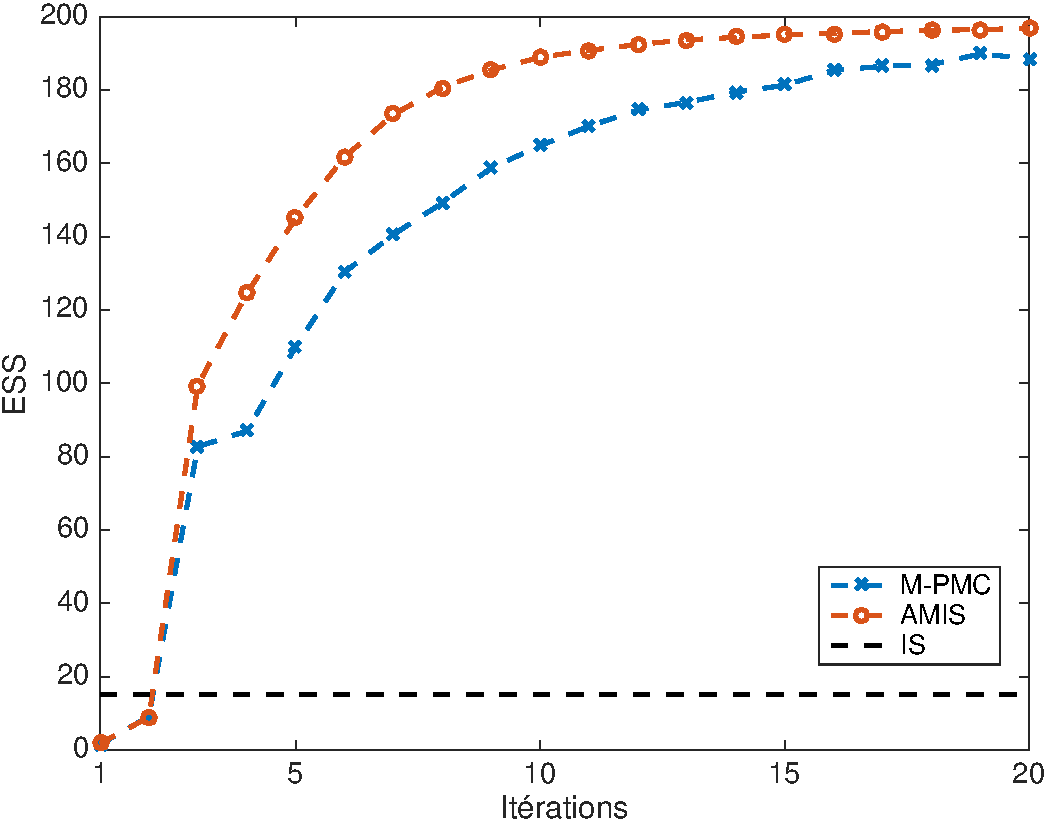
\includegraphics[width=0.8\textwidth]{mpmc_vs_amis}
		\end{figure}
	\end{columns}
\end{frame}

%% =====================================================================
\section{Application au cas expérimental FFT07}
%% =====================================================================
\begin{frame}
	\frametitle{L'expérience FFT07}
	Campagne expérimentale:
	\begin{itemize}
		\item rejets de gaz traceur sur terrain instrumenté dans diverses configurations (période, météo, nombre de sources...)
		\item création de données de référence pour validation d'algorithmes STE
	\end{itemize} 

			\begin{figure}
				\centering
				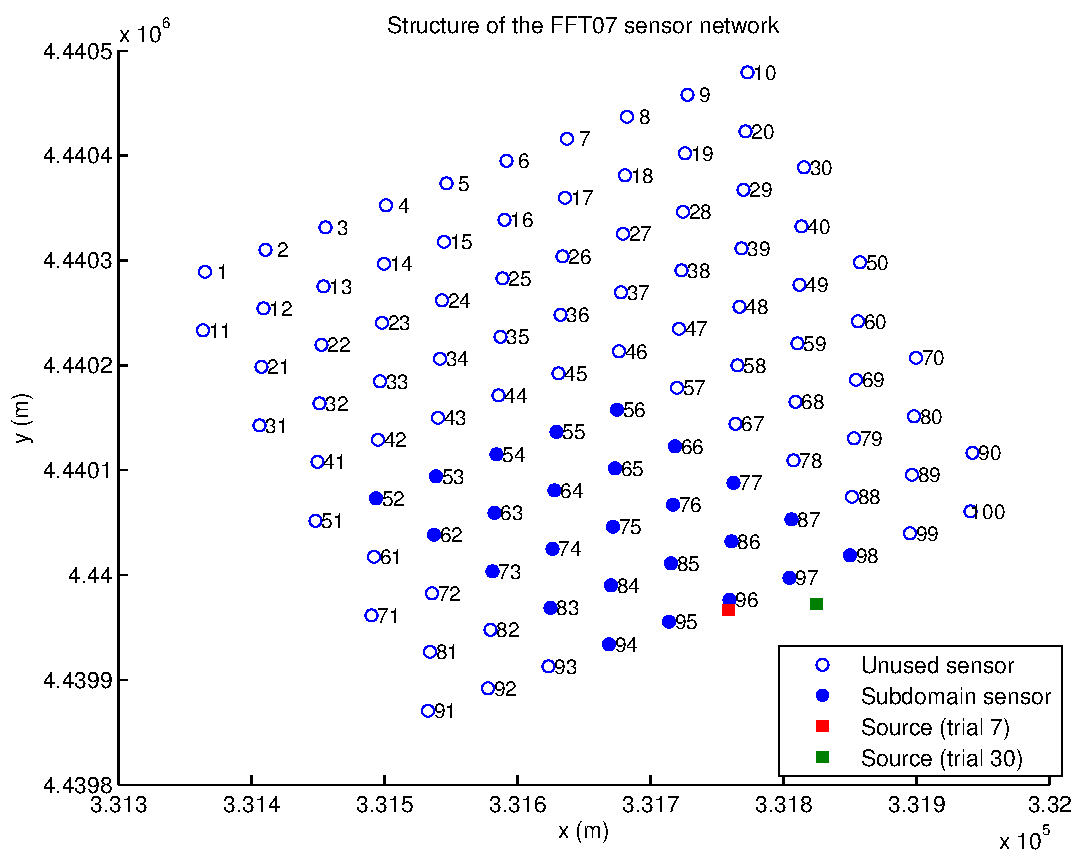
\includegraphics[width=0.65\textwidth]{fft07_capteurs}
			\end{figure}

\end{frame}
%% =====================================================================

\begin{frame}
	\frametitle{L'expérience FFT07}
	Caractéristiques des cas étudiés (\textit{trials} 7 et 30):
				\begin{itemize}
					\item  restriction à $N_C = 25$ capteurs proches de la source
					\item  $T_C$ instants d'observations moyennées sur fenêtres de 10s
					\item capteurs et source à même altitude: $\VecPosSource \in \mathbb{R}^2$
					\item rejet non-instantané, conditions atmosphériques stables
					\item étude avec données simulées et observations réelles
				\end{itemize}
	\begin{columns}
		\column[]{0.5\linewidth}
		Modèle de dispersion gaussien à bouffées:
		\begin{itemize}
			\item implémentation simple
			\item temps de calcul faibles
			\item émissions non-instantanées
			\item variabilité météorologique
		\end{itemize}
		\column[]{0.5\linewidth}
			\begin{figure}
				\centering
				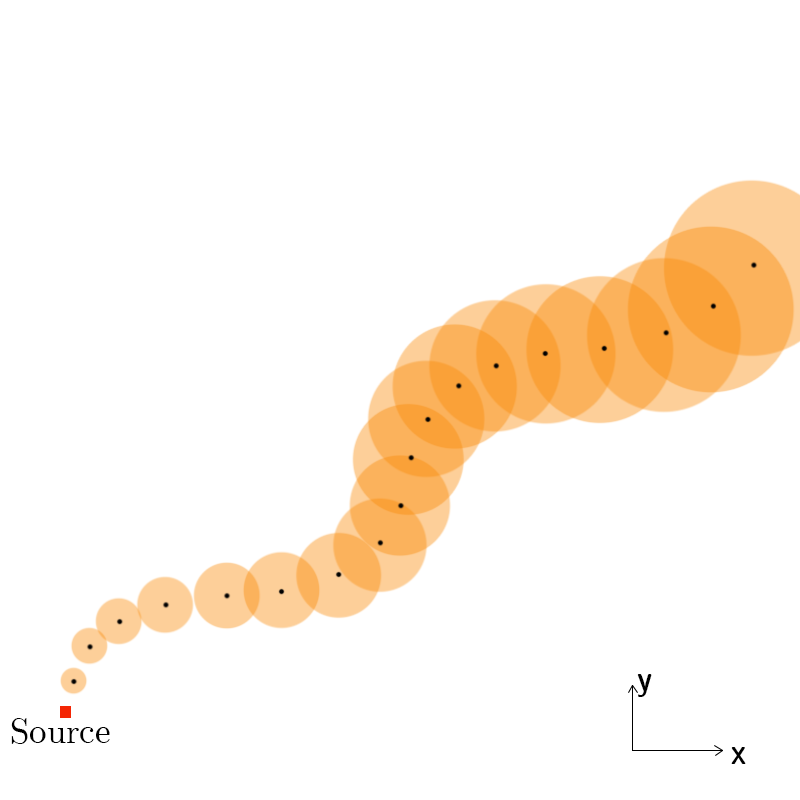
\includegraphics[width=0.75\textwidth]{gaussian_puff}
			\end{figure}
	\end{columns}
\end{frame}

%% =====================================================================

\begin{frame}
	\frametitle{Formalisation du problème STE}
	\textbf{Objectif}: estimer les paramètres de position $\VecPosSource$ et d'émission $\VecQSource$ de la source pour une configuration donnée (\textit{trial}) de l'expérience FFT07.\\
	\vspace{0.3cm}
	Modèle de données: 
	
	$$ \VecObs = \MatC(\VecPosSource)\VecQSource + \VecErreur $$
	
	où:
	\begin{itemize}
		\item $\VecObs \in \mathbb{R}^{N_CT_C}$: observations concaténées par capteur
		\item $\MatC(\VecPosSource) \in \mathbb{R}^{N_CT_C \times T_s}$: \textbf{matrice source-récepteur} construite avec un modèle de dispersion
		\item $\VecQSource \in \mathbb{R}^{T_s}$: profil d'émission
		\item $\VecErreur \in \mathbb{R}^{N_CT_C}$: erreurs (observation, modèle)
	\end{itemize}
\end{frame}
%% =====================================================================
\begin{frame}
	\frametitle{Formalisation du problème STE}
	\begin{figure}
		\centering
		\only<1>{
			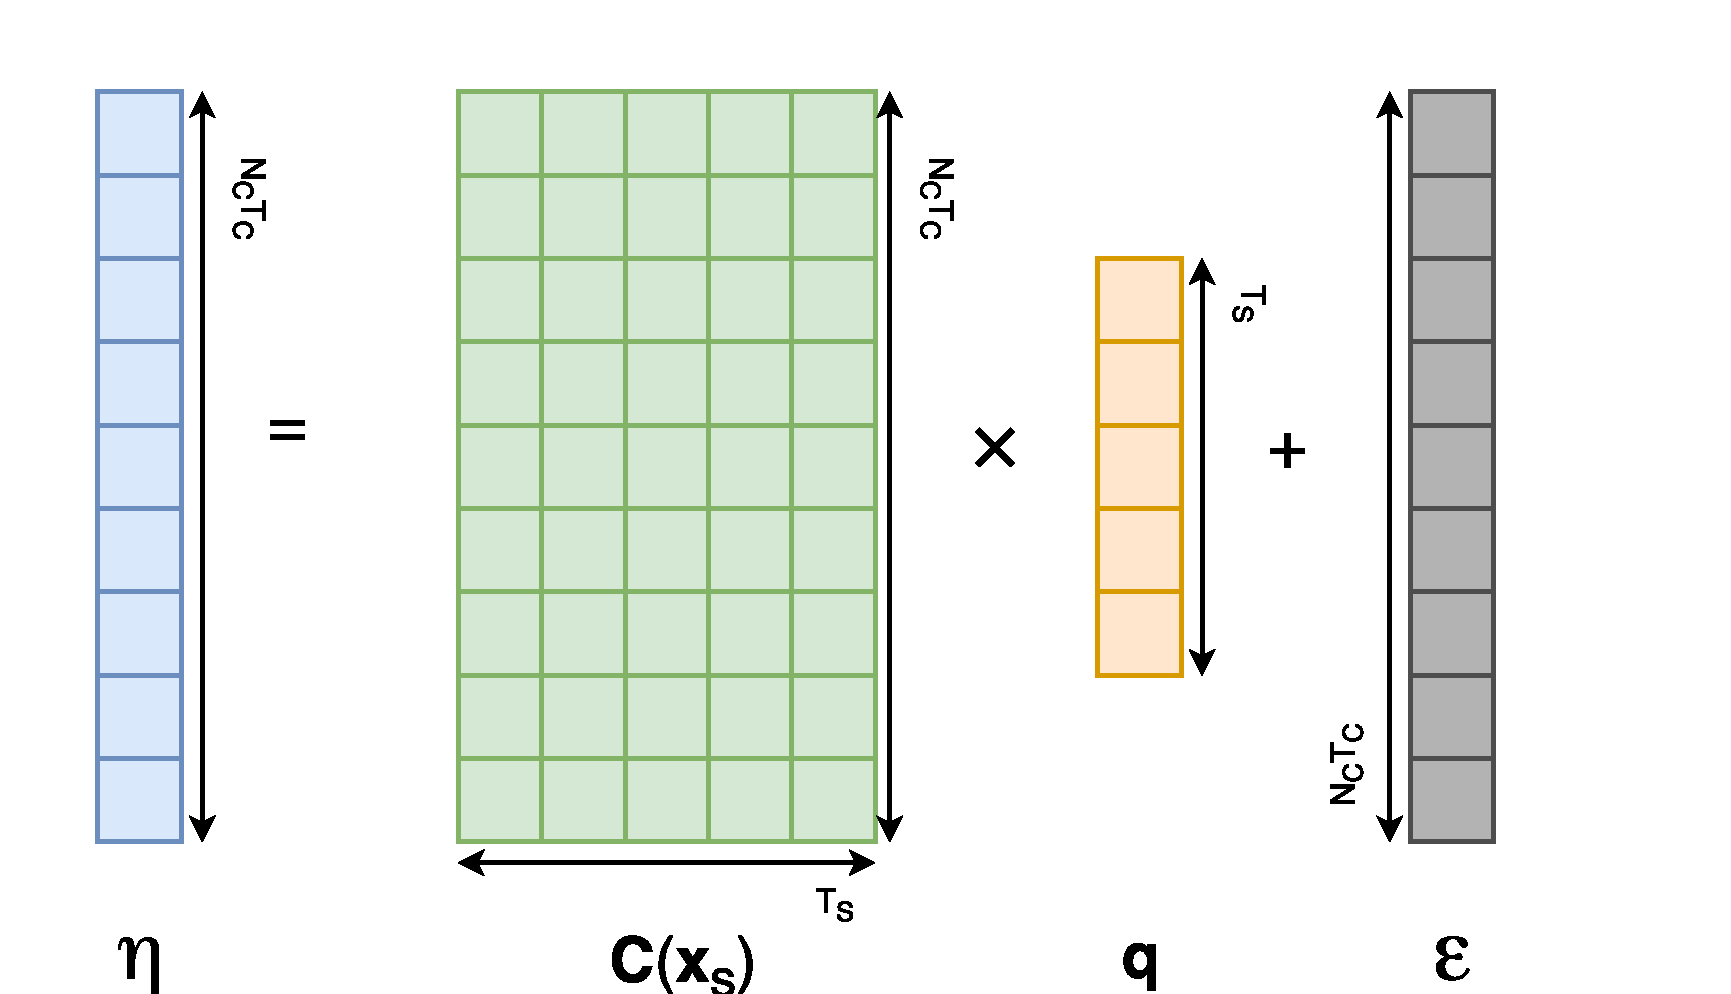
\includegraphics[width=0.99\textwidth]{data_model_initial}
		}
		\only<2>{
			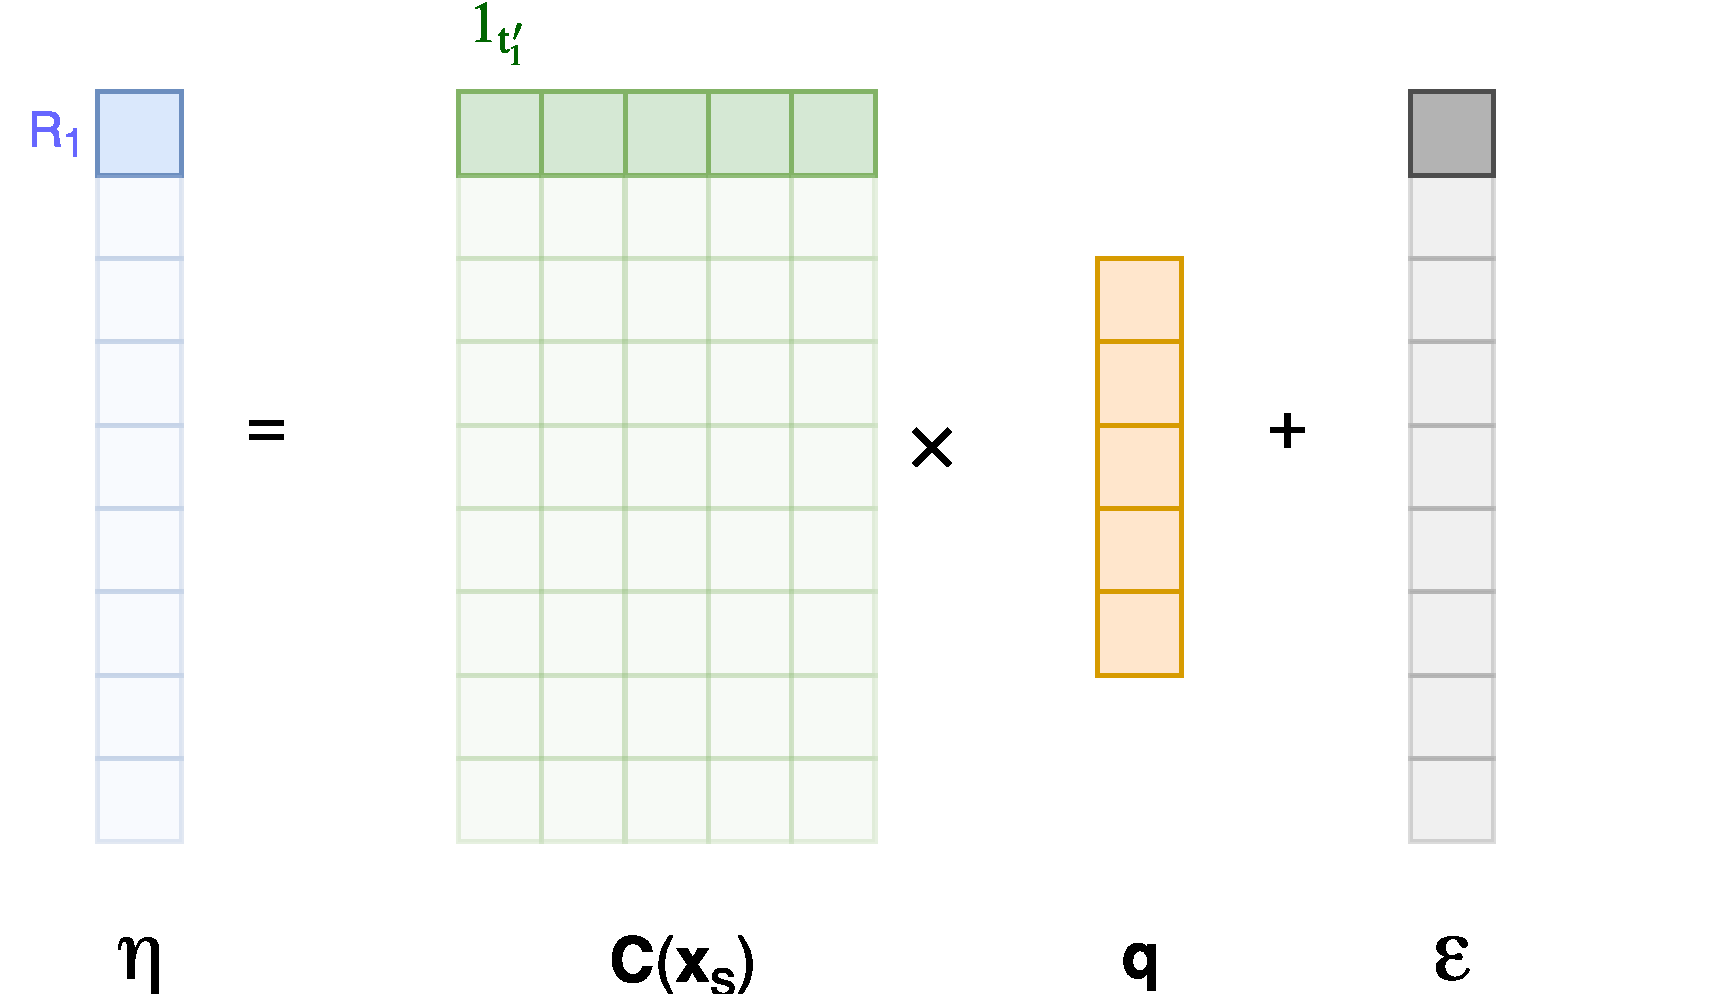
\includegraphics[width=0.99\textwidth]{data_model_step_1}
		}
		\only<3>{
			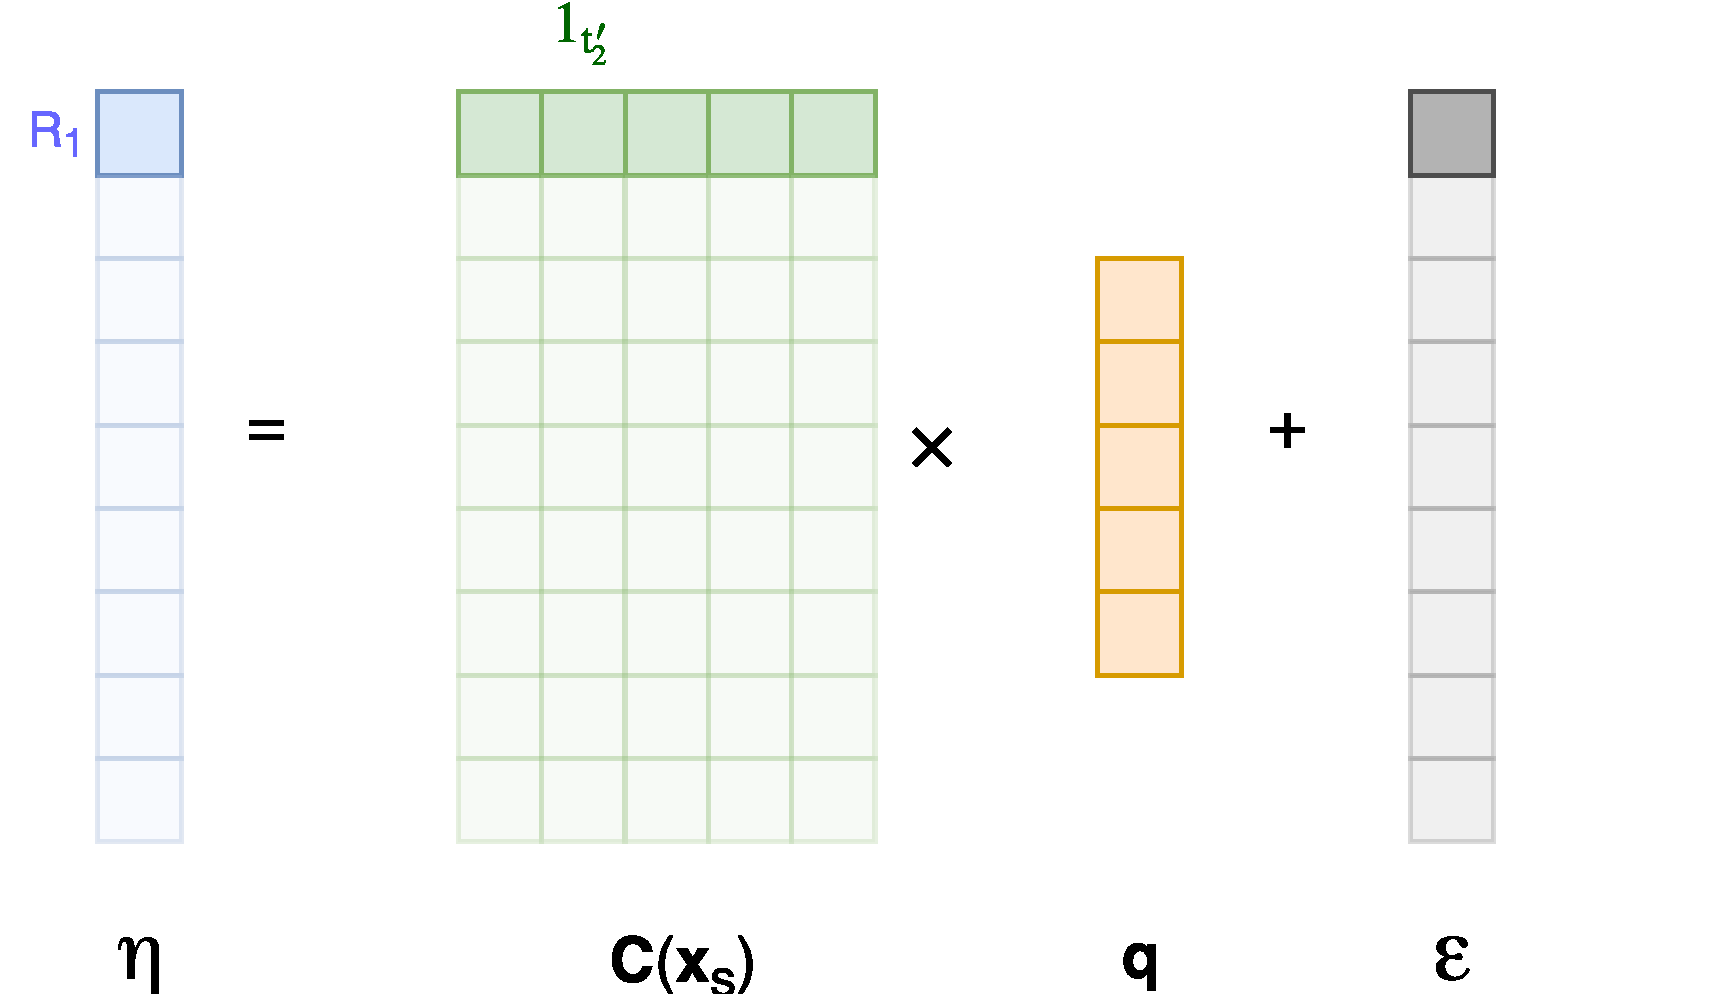
\includegraphics[width=0.99\textwidth]{data_model_step_2}
		}
		\only<4>{
			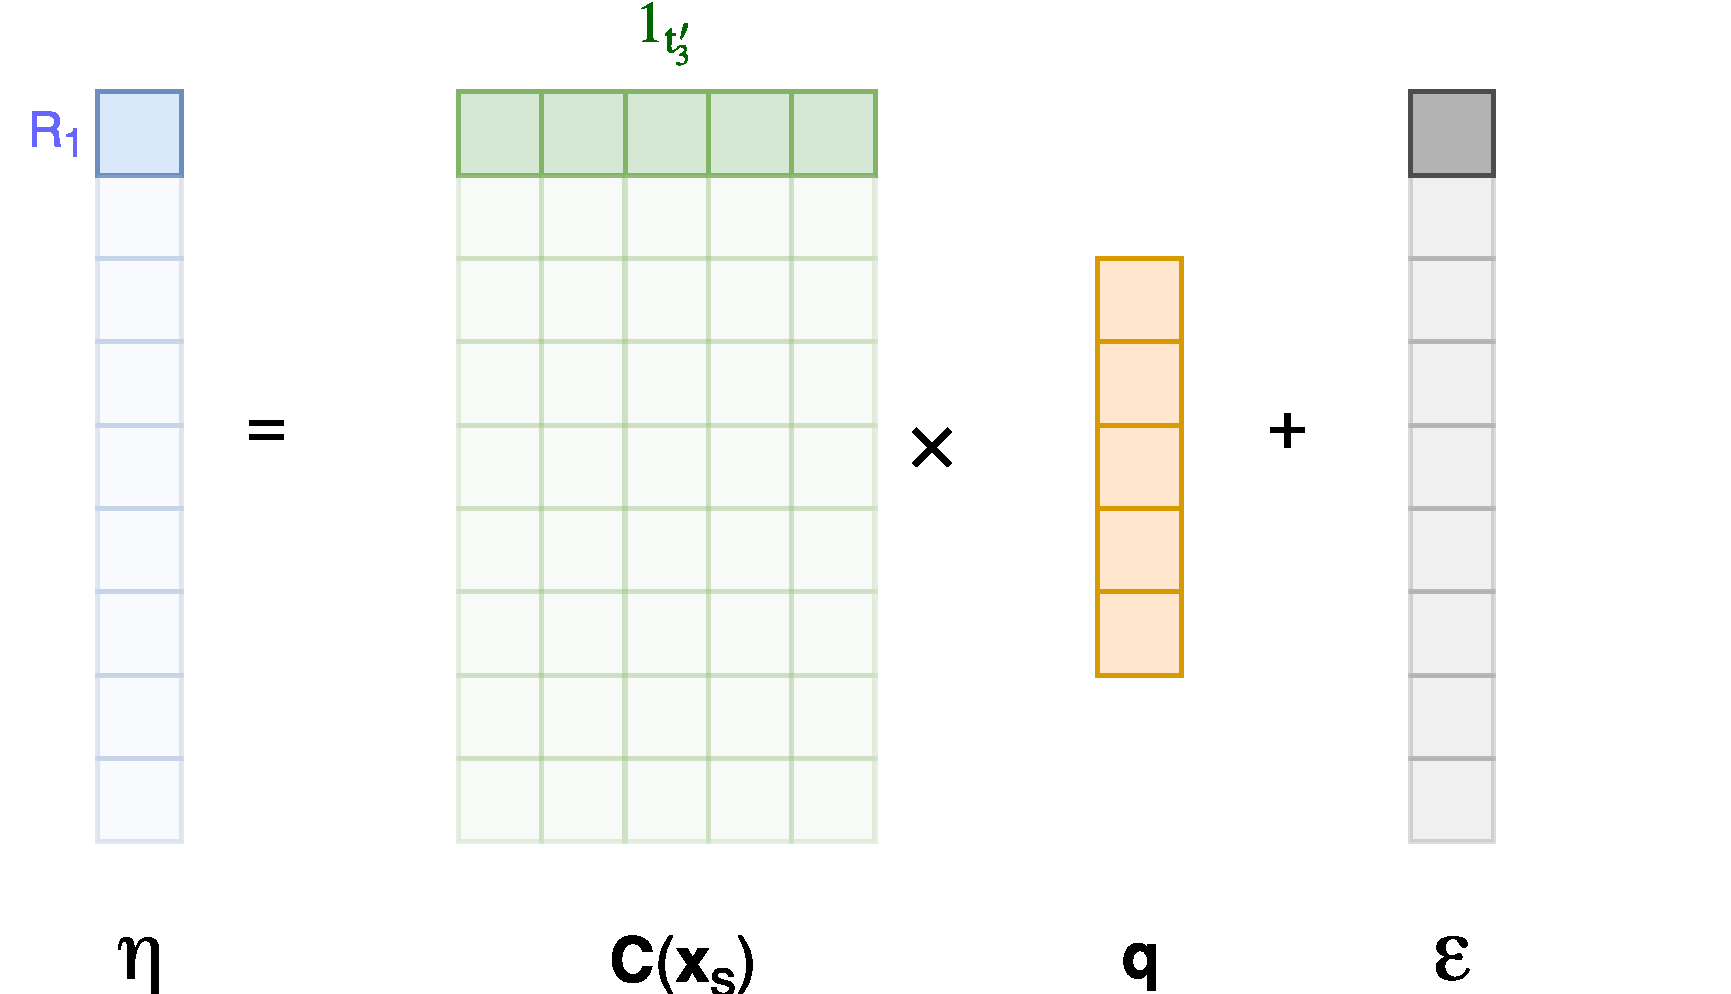
\includegraphics[width=0.99\textwidth]{data_model_step_3}
		}
		\only<5>{
			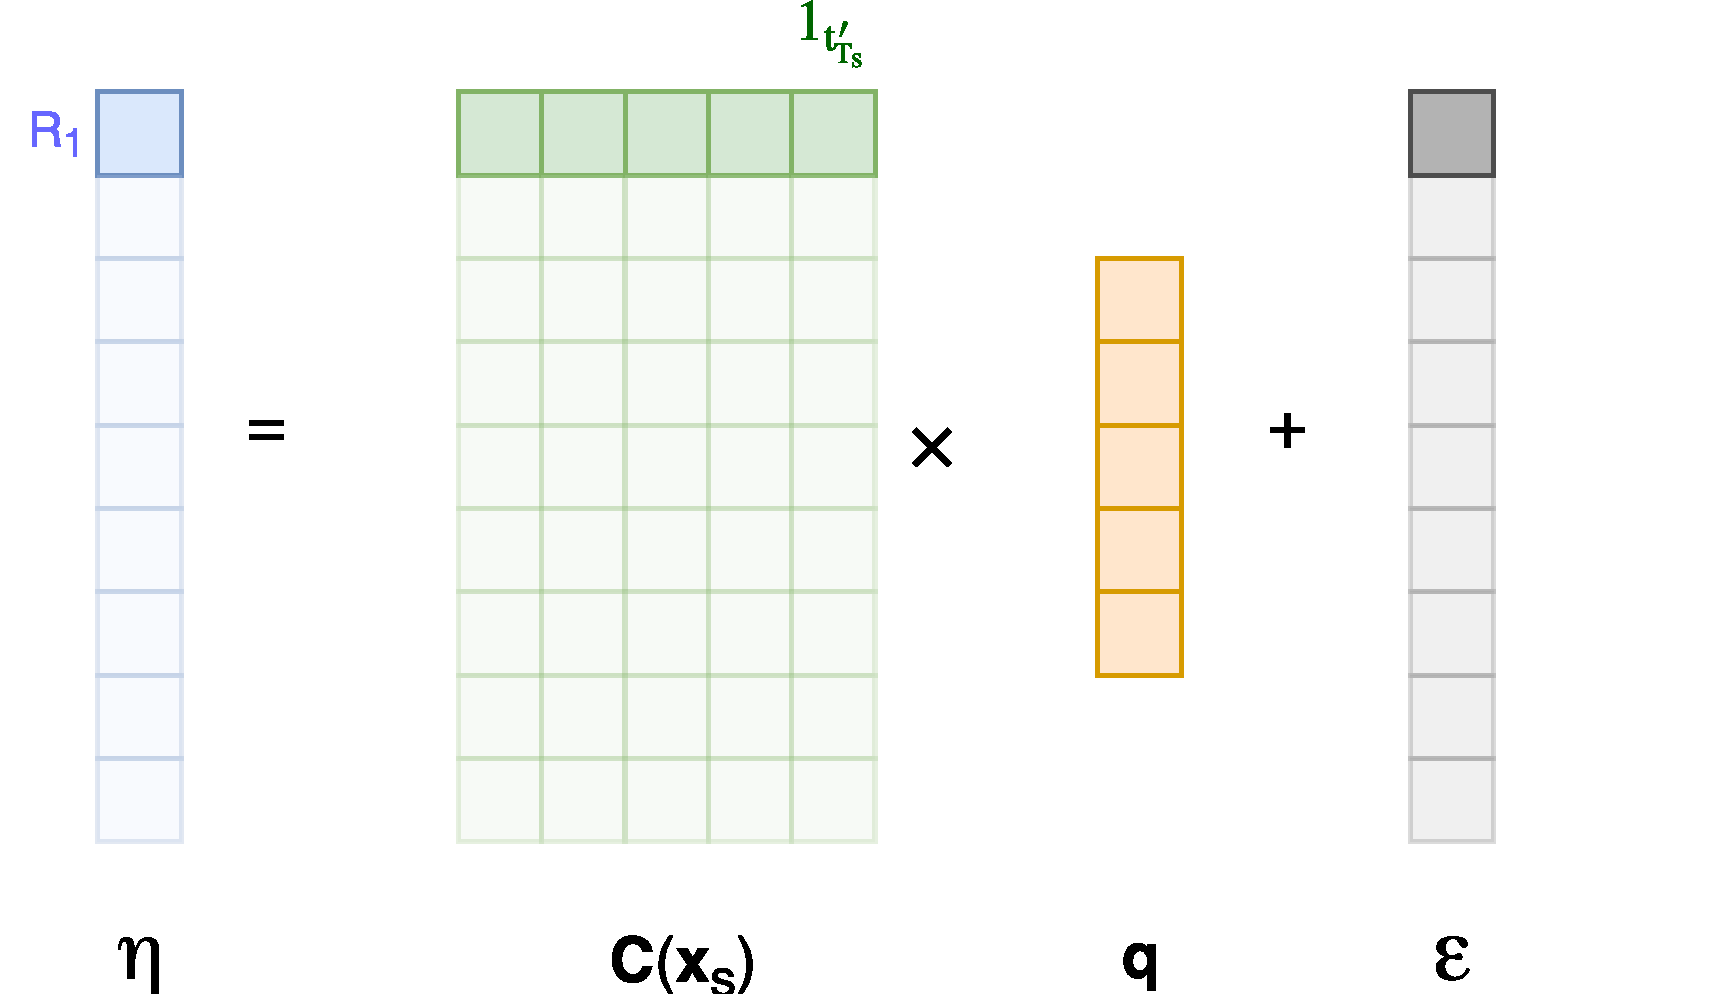
\includegraphics[width=0.99\textwidth]{data_model_step_4}
		}
		\only<6>{
			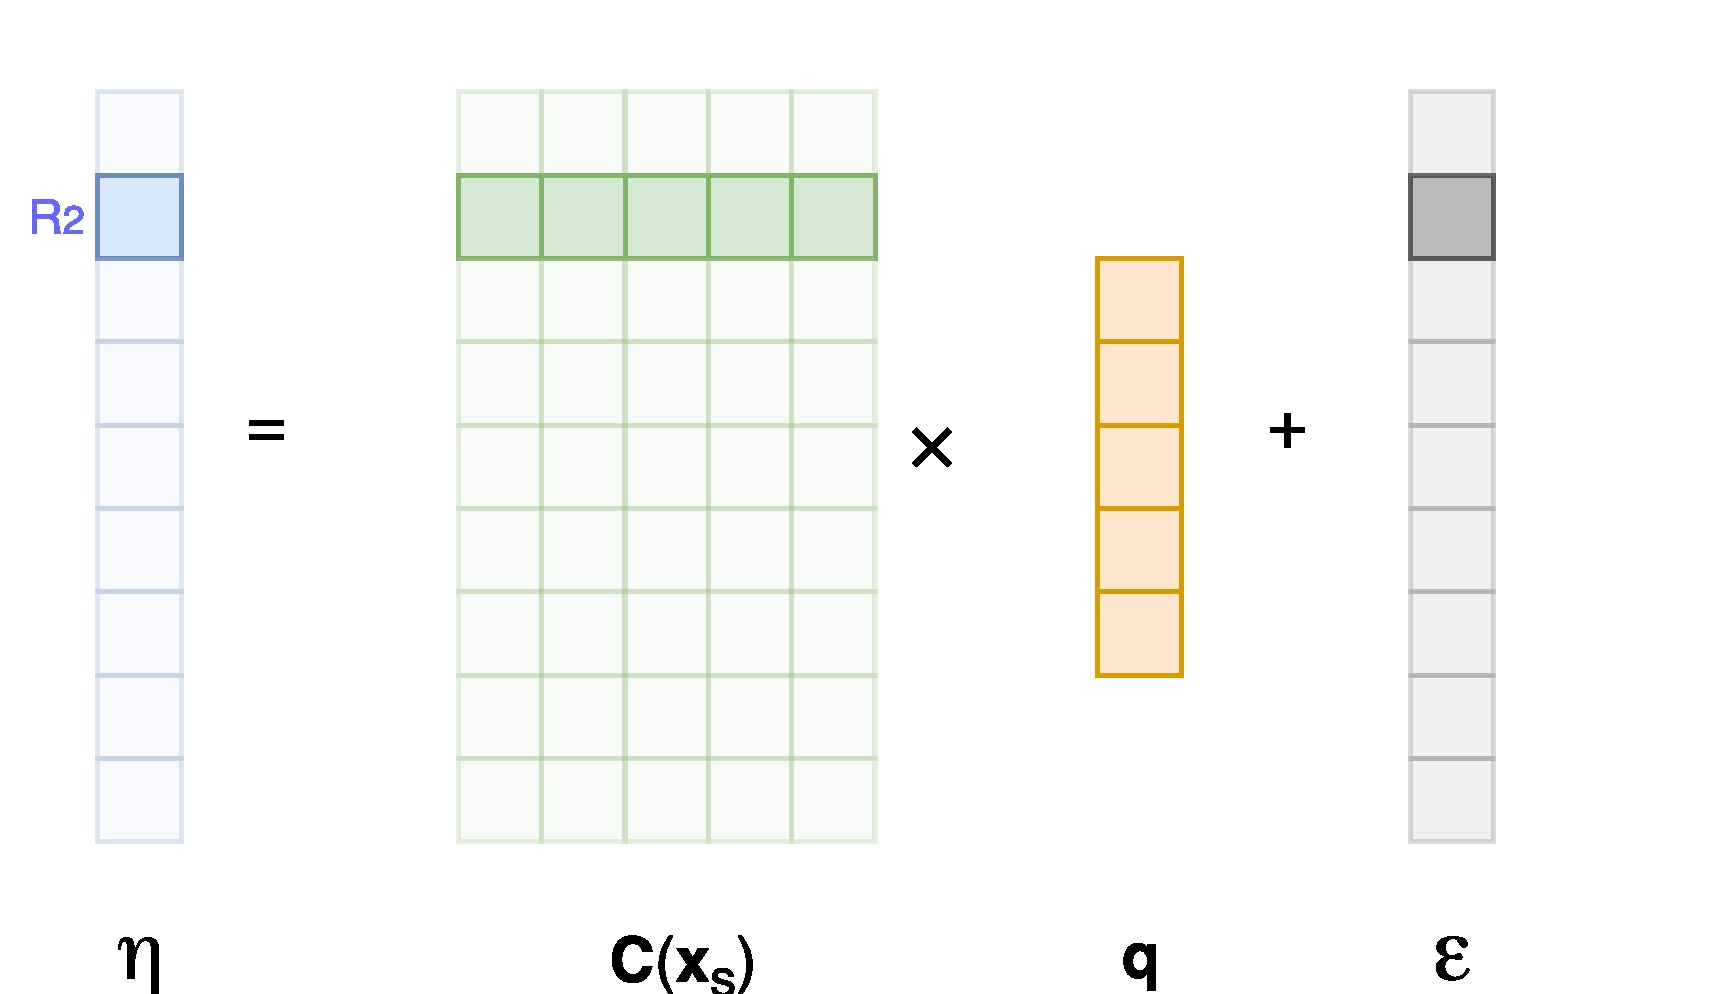
\includegraphics[width=0.99\textwidth]{data_model_step_5}
		}
		\only<7>{
			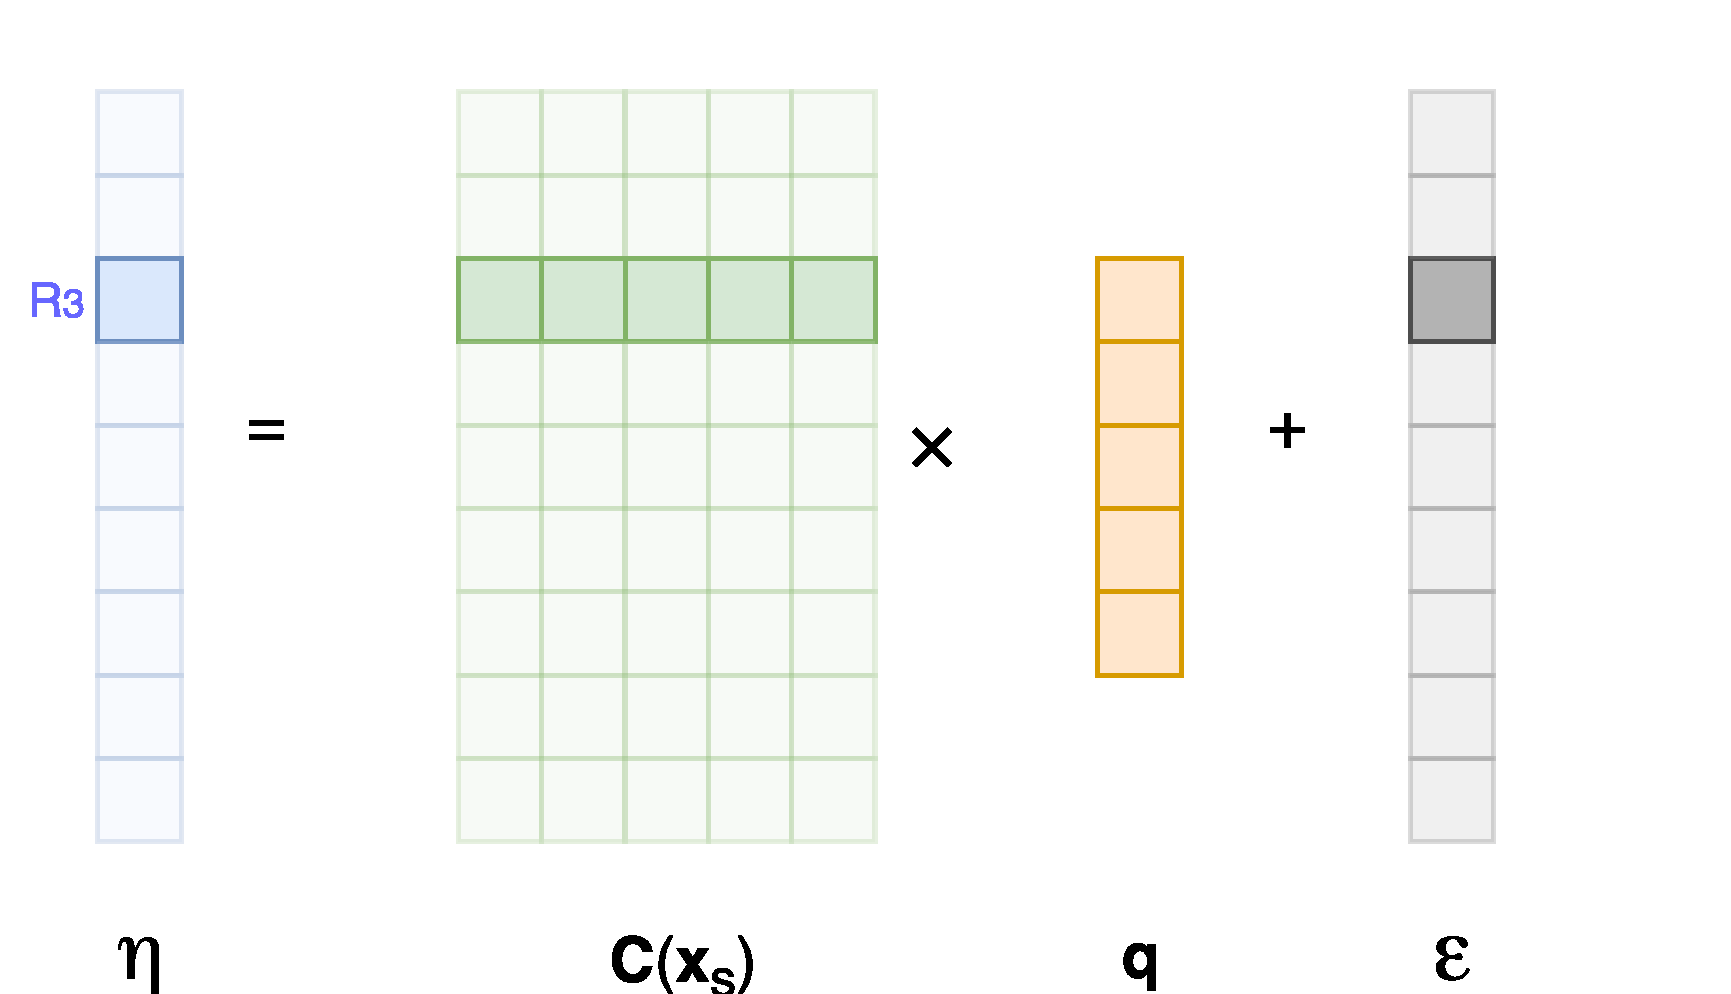
\includegraphics[width=0.99\textwidth]{data_model_step_6}
		}
		\only<8>{
			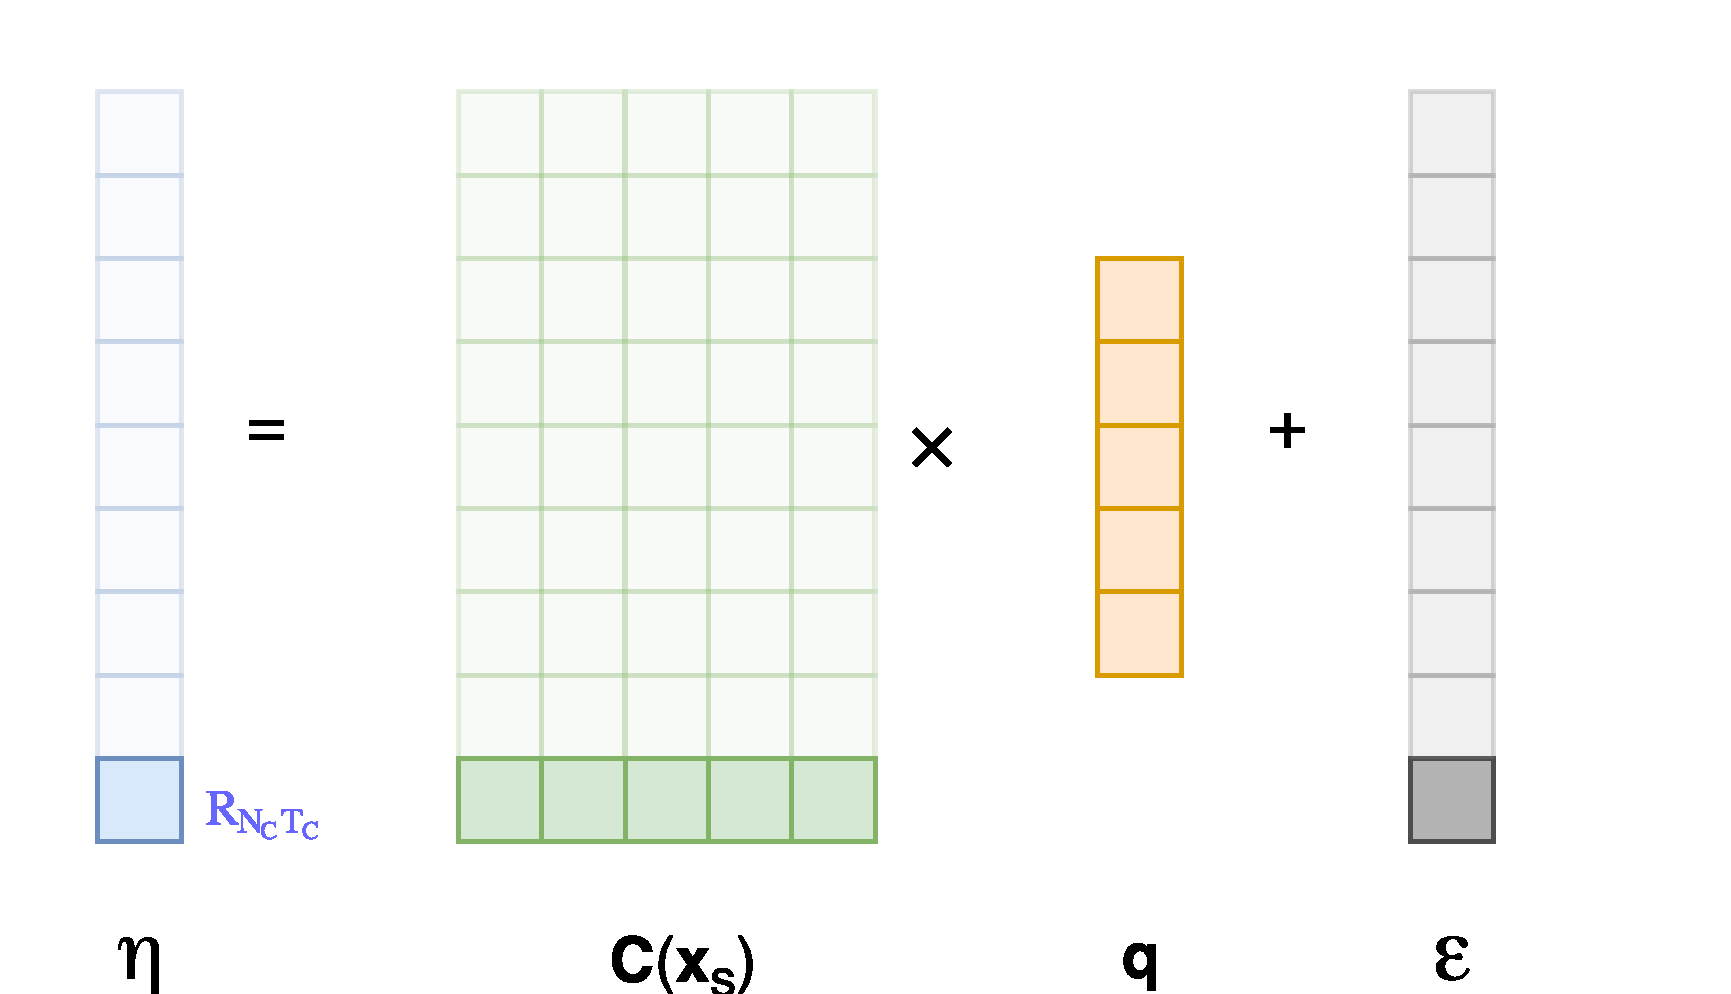
\includegraphics[width=0.99\textwidth]{data_model_step_7}
		}
	\end{figure}
\end{frame}
%% ======= ==============================================================
\begin{frame}
	\frametitle{Démarche de résolution}
	\begin{itemize}
		\item \textbf{Objectif}: calculer la loi a posteriori $p(\VecPosSource, \VecQSource | \VecObs)$ 
		\item \textbf{Problème}: source non-instantanée
		\begin{itemize}
			\item {\color{lightred}dimension $T_s + 2$ potentiellement élevée} du vecteur de paramètres,
			\item {\color{lightred}calcul coûteux} pour une simulation Monte-Carlo.
		\end{itemize}
	\end{itemize}
	\begin{greenblock}{Marginalisation du profil d'émission}
		La loi a posteriori des paramètres de la source peut s'écrire comme:
		$$p(\VecPosSource, \VecQSource | \VecObs) = p(\VecQSource | \VecPosSource, \VecObs)p(\VecPosSource | \VecObs) $$
		\begin{itemize}
			\item $p(\VecQSource | \VecPosSource, \VecObs)$: loi a posteriori conditionnelle de $\VecQSource$,
			\item $p(\VecPosSource | \VecObs)$: loi a posteriori marginale de $\VecPosSource$.
		\end{itemize} 
	\end{greenblock}
\end{frame}

%% ======= ==============================================================
\begin{frame}
	\frametitle{Démarche de résolution}
	La marginalisation permet de n'échantillonner que les $\VecPosSource$:
	\begin{figure}
		\centering
		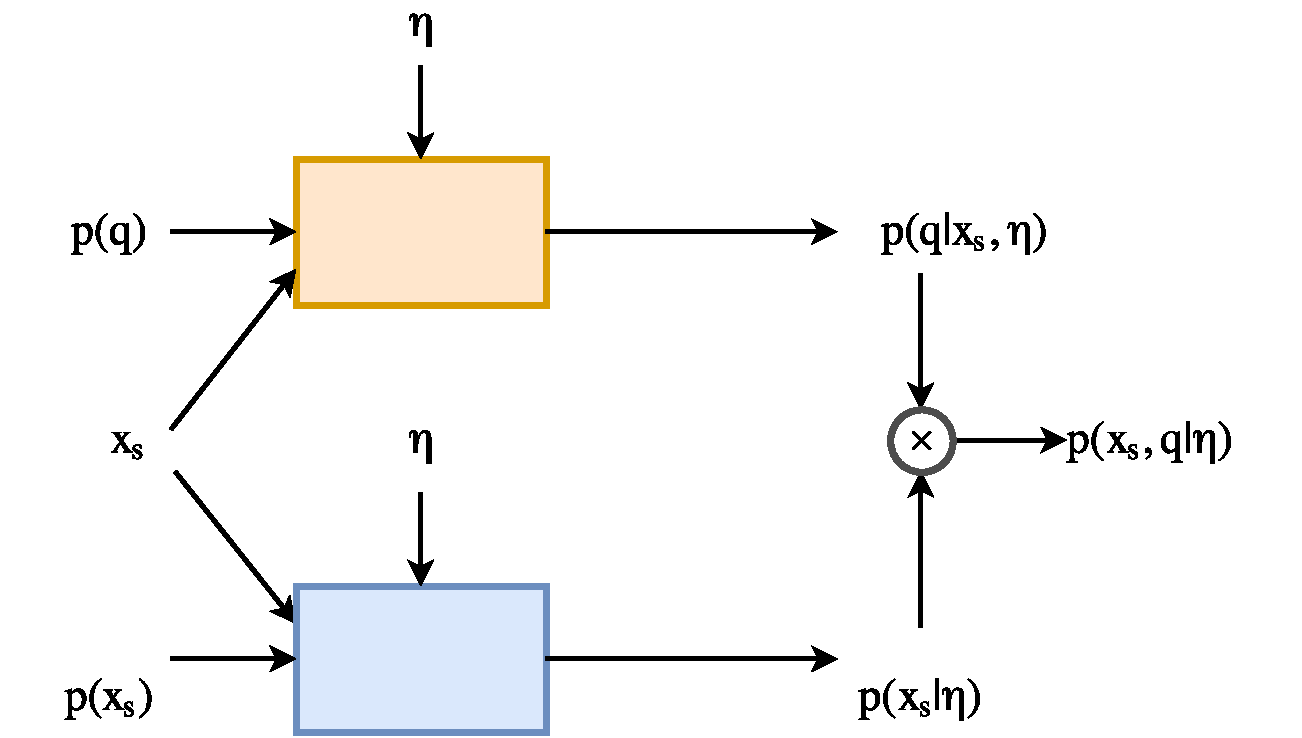
\includegraphics[width=1\textwidth]{bayesian_workflow_initial}
	\end{figure}
\end{frame}

%% ======= ==============================================================

\begin{frame}
	\frametitle{Loi conditionnelle de $\VecQSource$}
	\begin{figure}
		\centering
		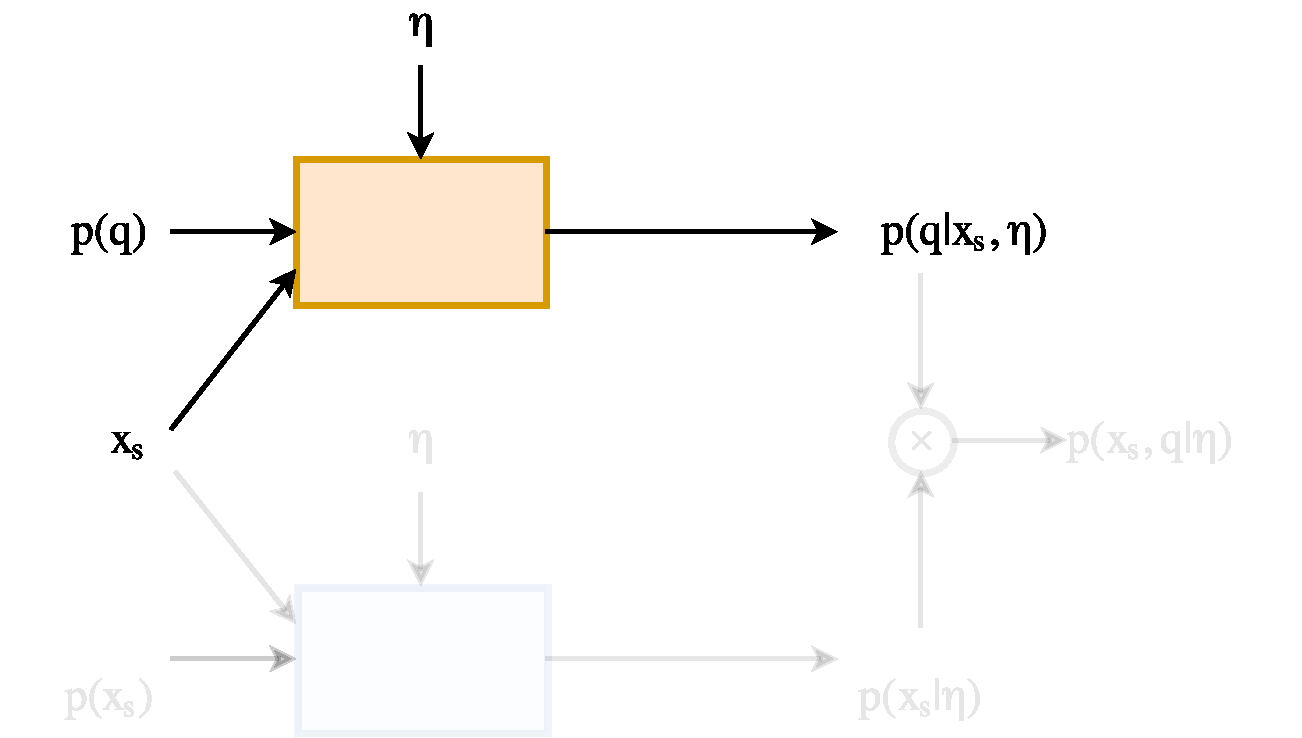
\includegraphics[width=1\textwidth]{bayesian_workflow_step_1}
	\end{figure}
\end{frame}
%% ======= ==============================================================

\begin{frame}
	\frametitle{Loi conditionnelle de $\VecQSource$}
	L'erreur sur $\VecObs$ est supposée gaussienne: $\VecErreur \sim \mathcal{N}(0, \sigma_{obs}^2\MatI)$  \\
	$\Rightarrow$ la vraisemblance est gaussienne: 
	$$ p(\VecObs | \VecPosSource, \VecQSource) = \prod_{i=1}^{N_c}\prod_{j=1}^{T_c} \mathcal{N}(\eta_{i,j} | \MatC_{i,j}(\VecPosSource)\VecQSource, \sigma_{obs}^2) $$
	
	\begin{greenblock}{A priori gaussien sur $\VecQSource$}
		Dans ces conditions, si $p(\VecQSource) = \mathcal{N}(\VecQSource | \VecMeanQ, \MatCovQ)$ alors : 
		$$ p(\VecQSource | \VecPosSource, \VecObs) = \mathcal{N}(\VecQSource | \PostMeanQ, \PostCovQ) $$
		
		avec $\PostMeanQ$ et $\PostCovQ$ obtenus analytiquement par résolution d'un système linéaire gaussien.
	\end{greenblock}
	
{\small 	\begin{itemize}
		\item hypothèse simplifiant la résolution du problème
		\item souvent employée dans la littérature STE
		\item {\color{lightred}perte potentielle de la positivité sur l'estimation de $\VecQSource$ !}
	\end{itemize}}
\end{frame}

%% ======= ==============================================================

\begin{frame}
	\frametitle{Loi conditionnelle de $\VecQSource$}
	\begin{greenblock}{Contrainte de positivité par troncature de la densité}
		% Troncature sans changer la nature gaussienne de la PDF
		\textbf{Objectif}: restreindre $p(\VecQSource | \VecPosSource, \VecObs)$ à des valeurs positives en conservant la nature gaussienne de la densité d'origine.
		\begin{itemize}
			\item assure la cohérence physique de la solution
			\item {\color{lightred}rallonge le temps de calcul}
			\item {\color{lightred}modifie potentiellement les valeurs initiales}
		\end{itemize}
	\end{greenblock}
	
	Exemples sur lois gaussiennes bivariées:
	\begin{figure}
		\centering
		\begin{subfigure}[b]{0.31\textwidth}
			\centering
			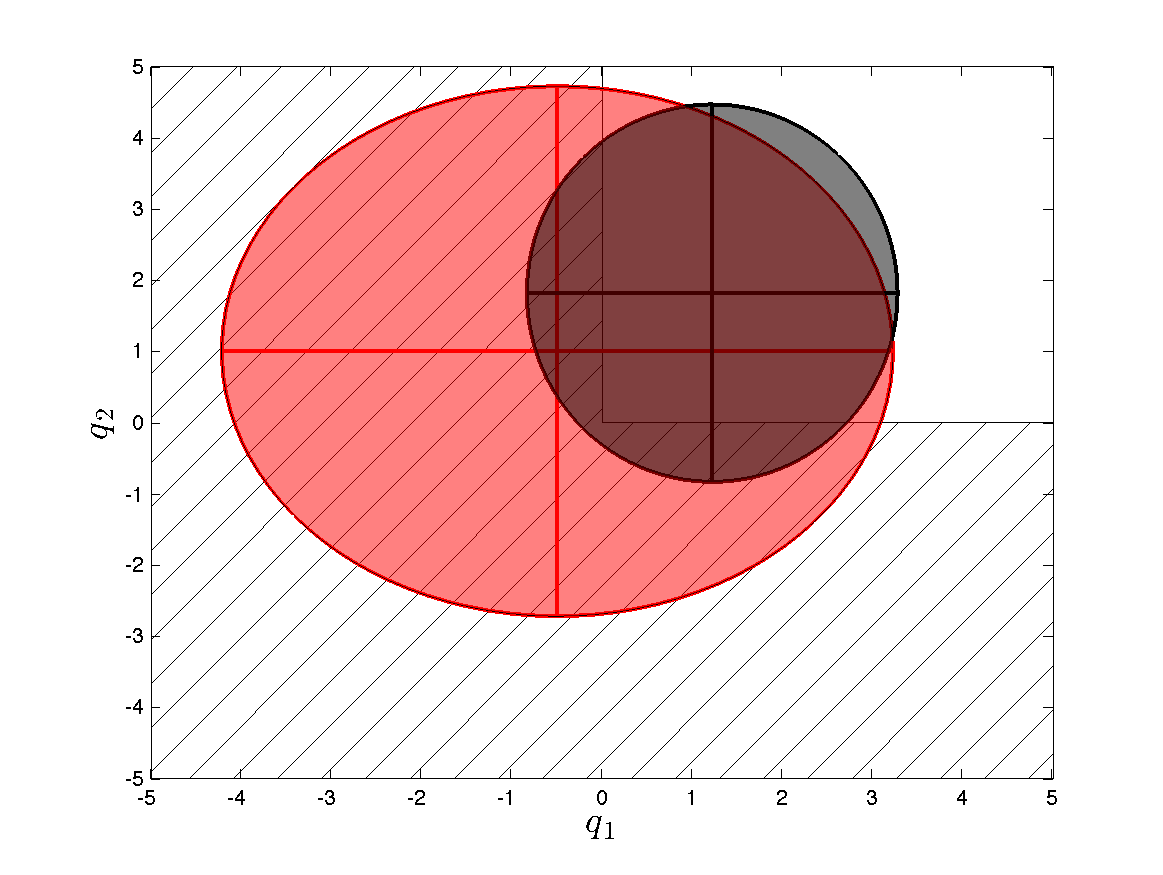
\includegraphics[width=\textwidth]{contrainte_positivite_1}
		\end{subfigure}
		\hfill
		\begin{subfigure}[b]{0.31\textwidth}
			\centering
			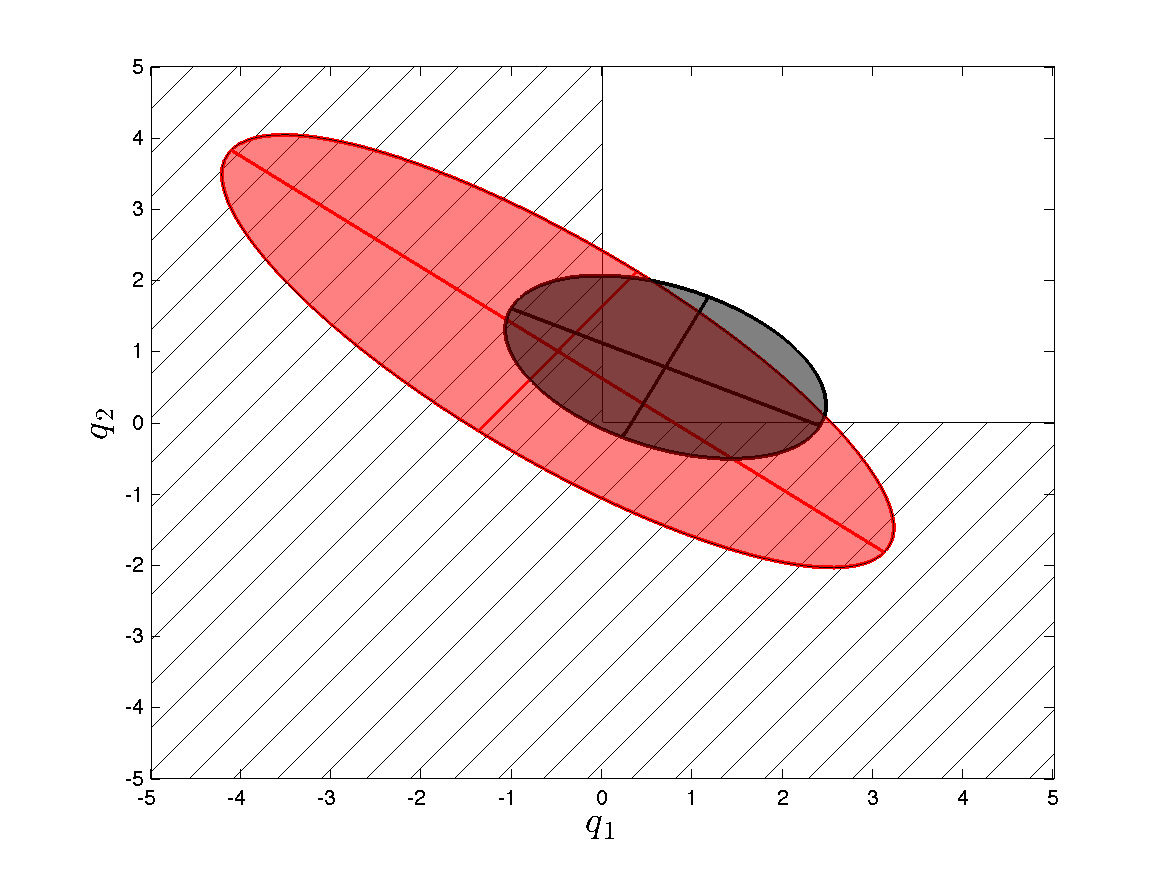
\includegraphics[width=\textwidth]{contrainte_positivite_2}
		\end{subfigure}
		\hfill
		\begin{subfigure}[b]{0.31\textwidth}
			\centering
			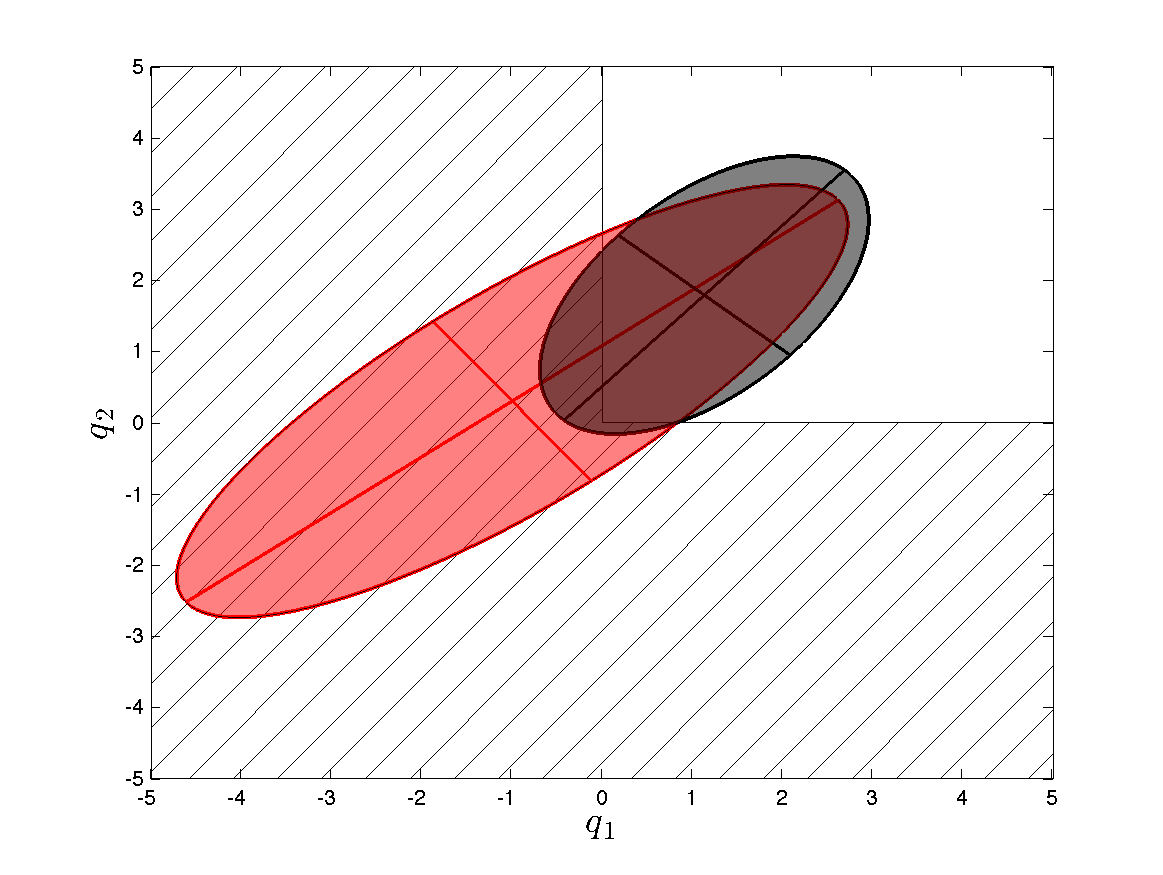
\includegraphics[width=\textwidth]{contrainte_positivite_3}
		\end{subfigure}
	\end{figure}
\end{frame}
%% ======= ==============================================================

\begin{frame}
	\frametitle{Loi conditionnelle de $\VecQSource$}
	\begin{figure}
		\centering
		\only<1>{
			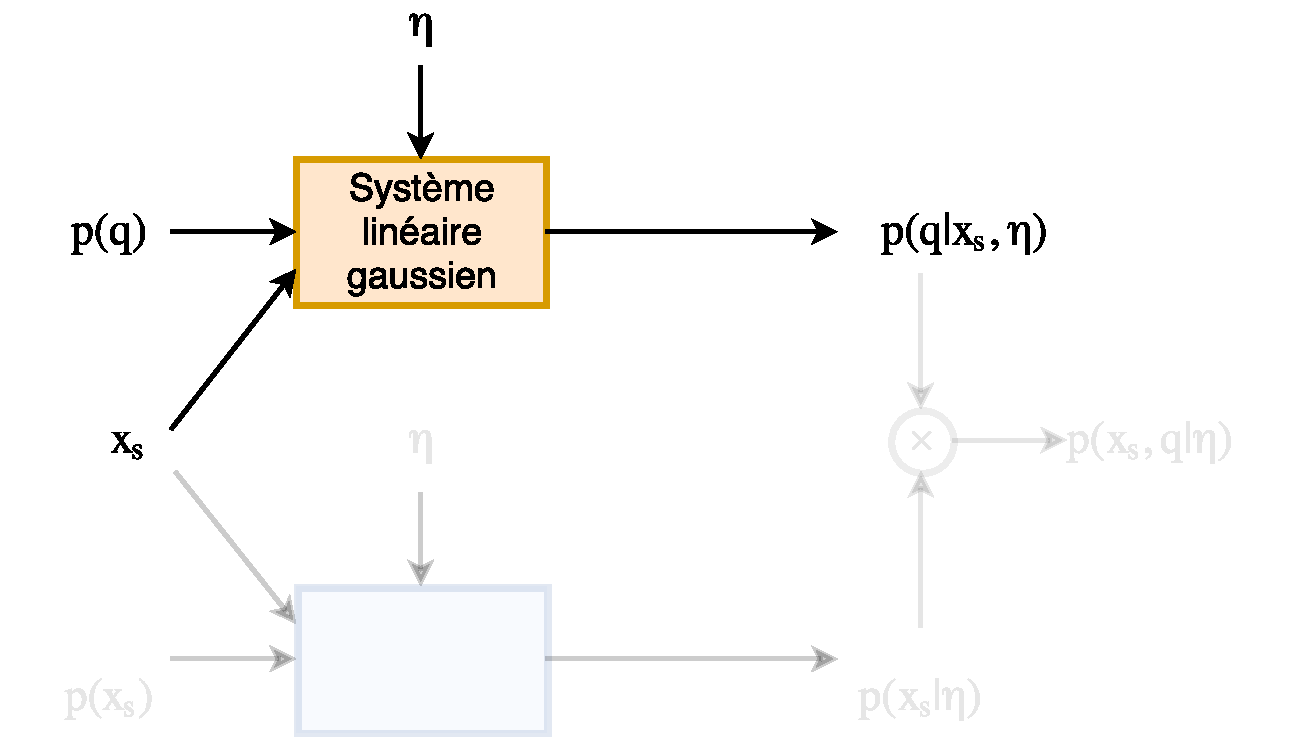
\includegraphics[width=1\textwidth]{bayesian_workflow_step_1_end}
			}
		\only<2>{
			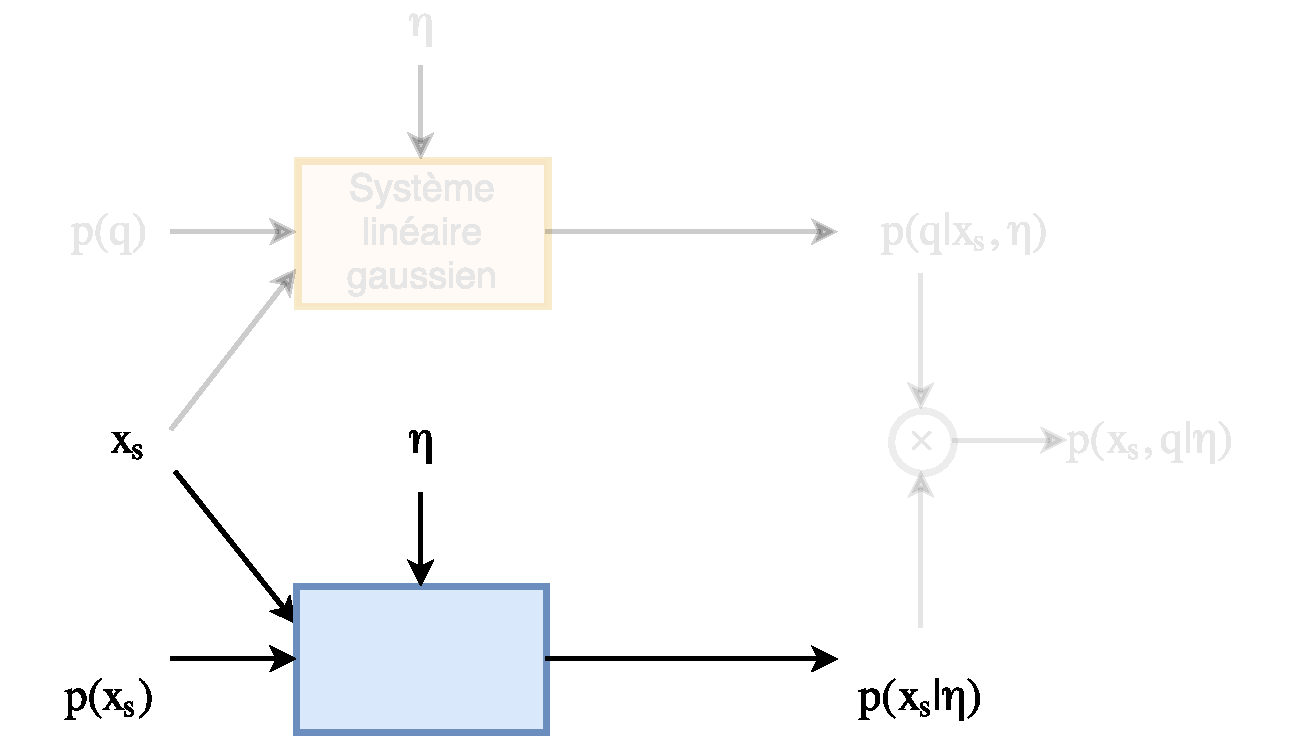
\includegraphics[width=1\textwidth]{bayesian_workflow_step_2}
			}
	\end{figure}
\end{frame}
%% ======= ==============================================================

\begin{frame}
	\frametitle{Loi a posteriori marginale de $\VecPosSource$}
	On utilise l'AMIS pour calculer $p(\VecPosSource | \VecObs)$:
	\begin{itemize}
		\item génération d'un échantillon de $KN_p$ particules sur $K$ itérations
		\item loi a priori $p(\VecPosSource)$ uniforme sur le domaine
		\item loi de proposition $\varphi_{\alpha, \nu}$: 
		\begin{itemize}
			\item mélange de $D=4$ noyaux gaussiens
			\item paramètres $\big(\alpha_d, \nu_d = \{\VecMu_d, \MatSigma_d\}\big)_{1\leq d \leq D}$ optimisés à chaque itération
		\end{itemize} 
		\item initialisation de  $\varphi_{\alpha, \nu}$: répartition homogène sur le domaine 
			\begin{figure}
				\centering
				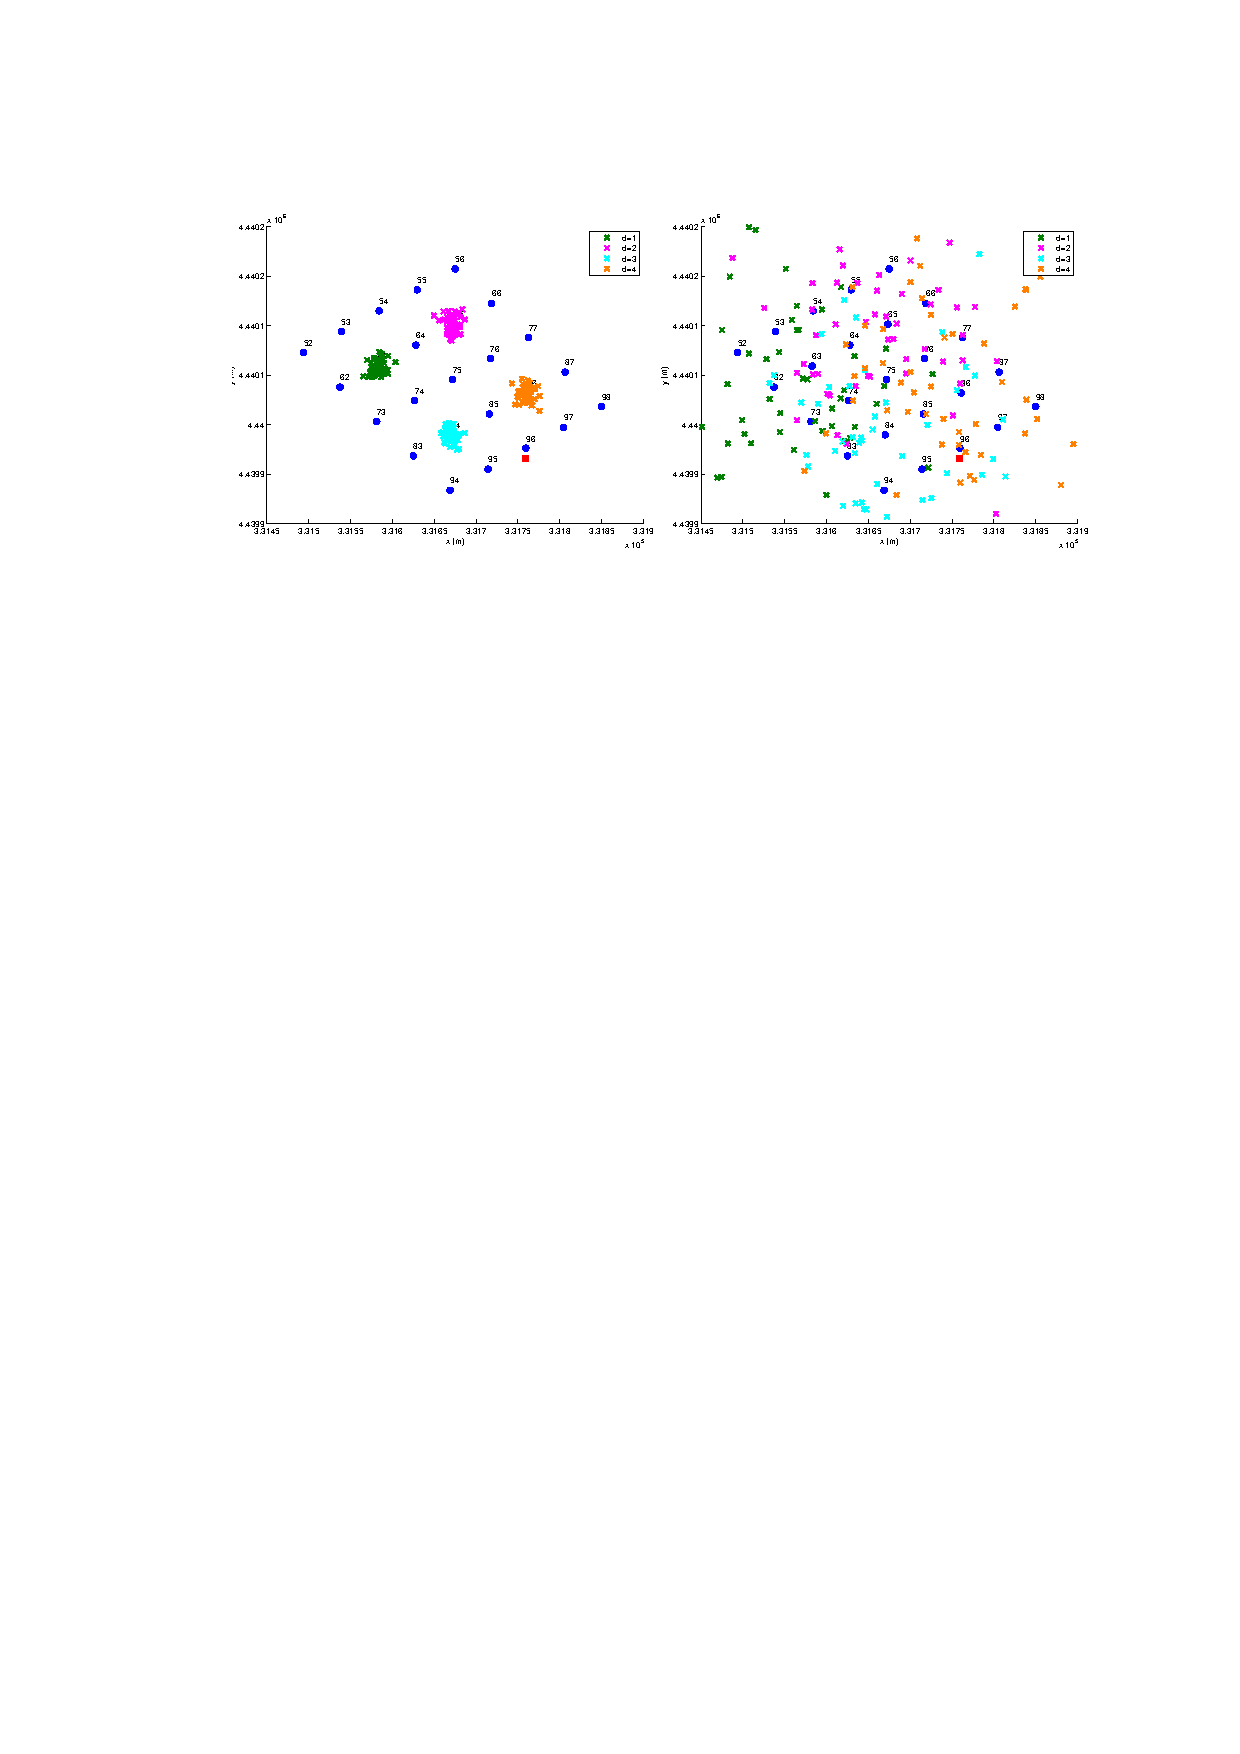
\includegraphics[width=0.75\textwidth]{initialisation_amis}
			\end{figure}
	\end{itemize}

\end{frame}
%% ======= ==============================================================

\begin{frame}
	\frametitle{Loi a posteriori marginale de $\VecPosSource$}
	Fonctionnement de l'AMIS sur 1 itération:
	\begin{figure}
		\centering
		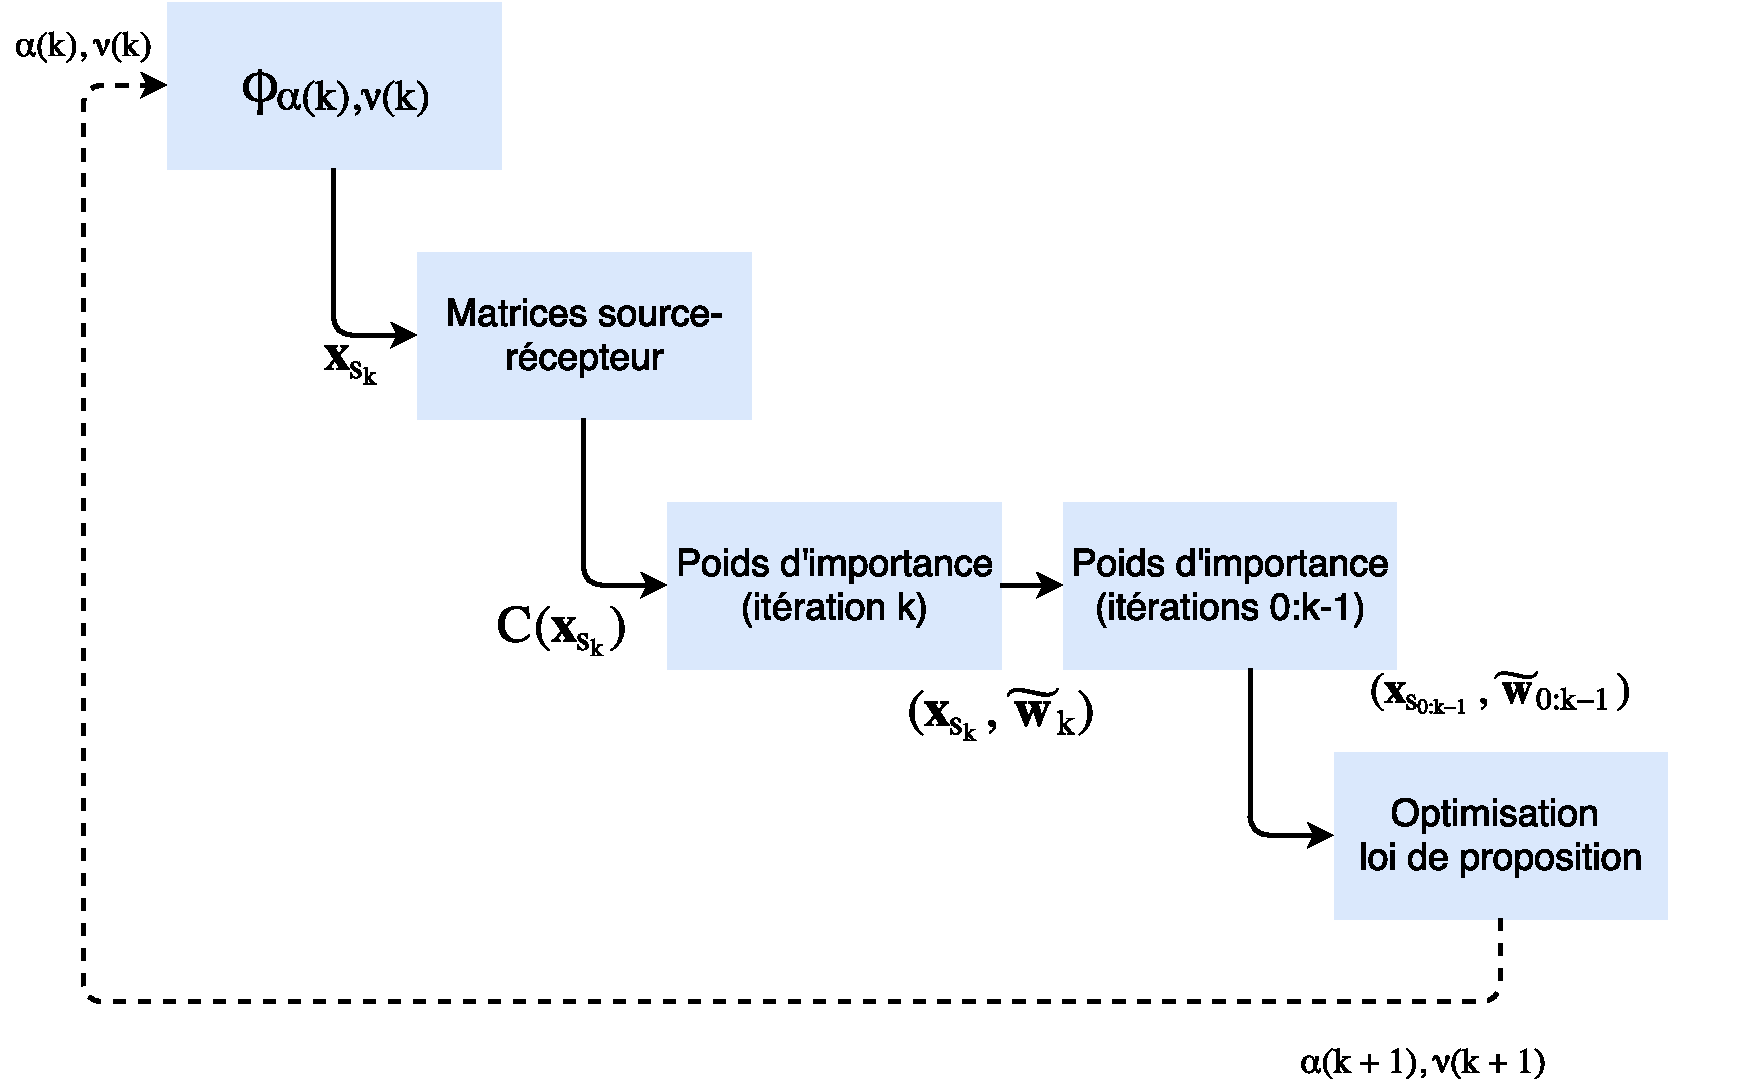
\includegraphics[width=1\textwidth]{amis_workflow}
	\end{figure}
\end{frame}

\begin{frame}
	\frametitle{Loi conditionnelle de $\VecQSource$}
	\begin{figure}
		\centering
			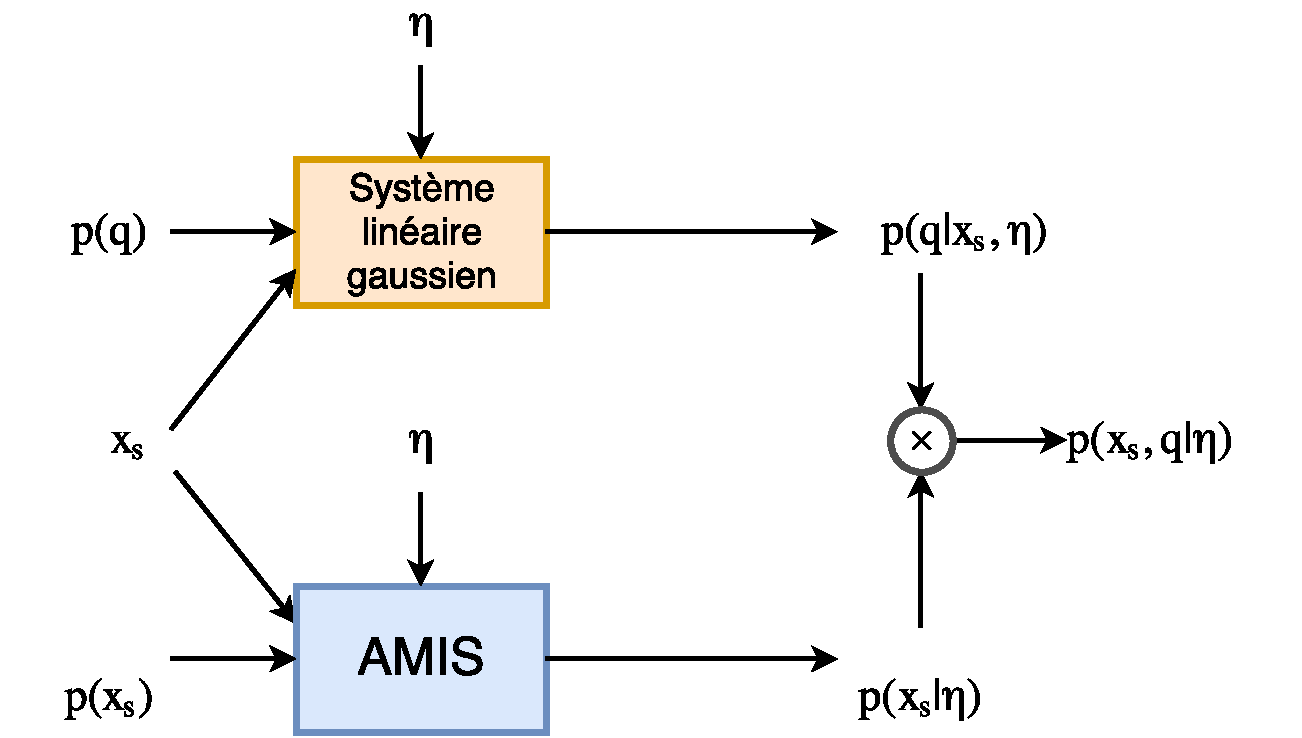
\includegraphics[width=1\textwidth]{bayesian_workflow_final}

	\end{figure}
\end{frame}
%% =======

%% ======= ==============================================================

\begin{frame}
	\frametitle{Résultats (observations simulées)}
	Position estimée par l'AMIS pour un rejet non-instantané:
	\begin{figure}
		\centering
		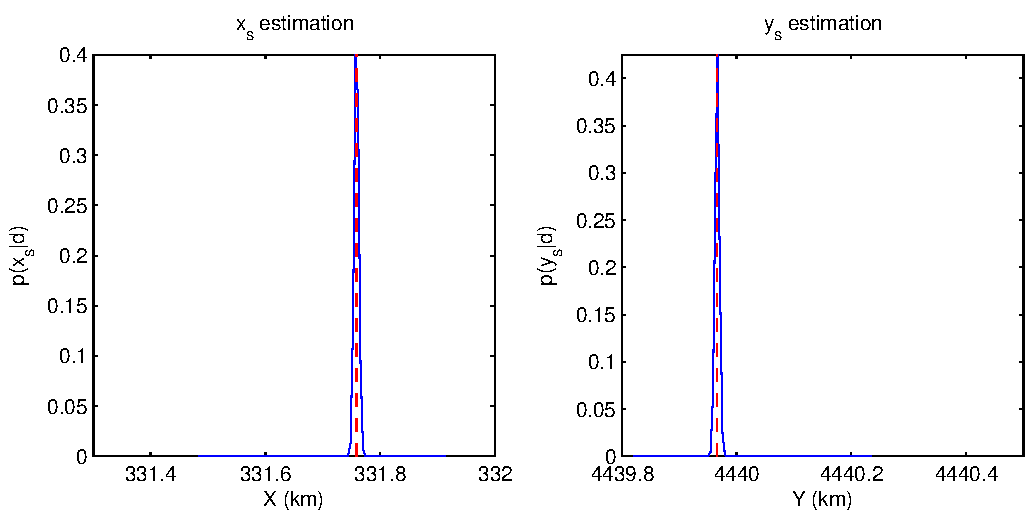
\includegraphics[width=0.8\linewidth]{res_fft07_simu_position}
	\end{figure}
	\begin{columns}
		\column[]{0.45\linewidth}
			\begin{greenblock}{Estimateur MMSE (position)}
			$$ \widehat{\VecPosSource} = \sum\limits_{k=1}^K\sum\limits_{i=1}^{N_p} \widetilde{w}_k^{(i)}\VecPosSource_k^{(i)}$$
			\end{greenblock}

		\column[]{0.55\linewidth}
		
		Contrainte de positivité: \\
		\vspace{0.5cm}
{\small 		\begin{tabular}{c|ccc}
			\centering
			&  $\bar{d}(\widehat{\VecPosSource}, \bm{x}_{s^T}) $ & $\sigma_{\widehat{x_s}}$ (m) & $\sigma_{\widehat{y_s}}$ (m)  \\ 
			\hline 
			Avec  &  $\leq 1$ & $0.9$  & $3.2$ \\
			Sans & $10.44$ & $0.4$ & $1.0$
		\end{tabular} 
			}
	\end{columns}

\end{frame}


%% ======= ==============================================================

\begin{frame}
	\frametitle{Résultats (observations simulées)}
	\begin{greenblock}{Estimateur MMSE (profil émission)}
		$$ \widehat{\VecQSource} = \sum\limits_{k=1}^K\sum\limits_{i=1}^{N_p} \widetilde{w}_k^{(i)} \widetilde{\VecMu}(\VecPosSource_k^{(i)}) $$		
	\end{greenblock}
	
	Différents profils estimés, avec contrainte de positivité:
	
	\begin{figure}
		\centering
		\begin{subfigure}[b]{0.33\textwidth}
			\centering
			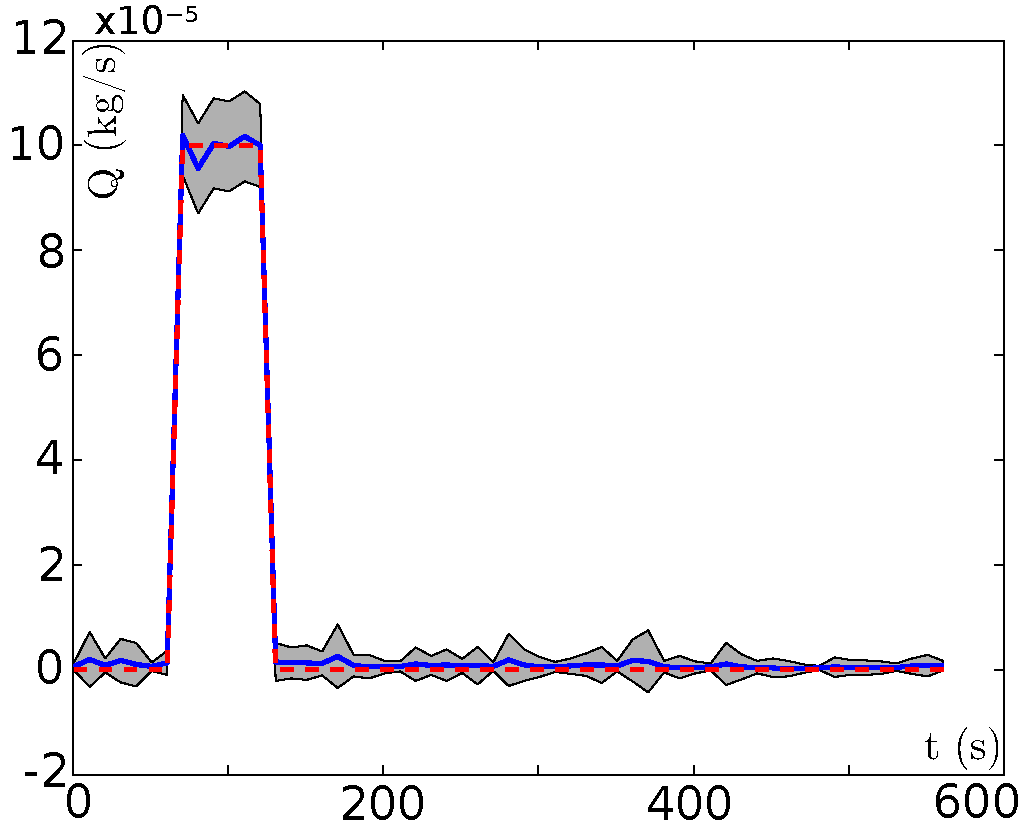
\includegraphics[width=\textwidth]{res_fft07_simu_q_1}
			\caption*{non-instantané}
		\end{subfigure}
		\hfill
		\begin{subfigure}[b]{0.3\textwidth}
			\centering
			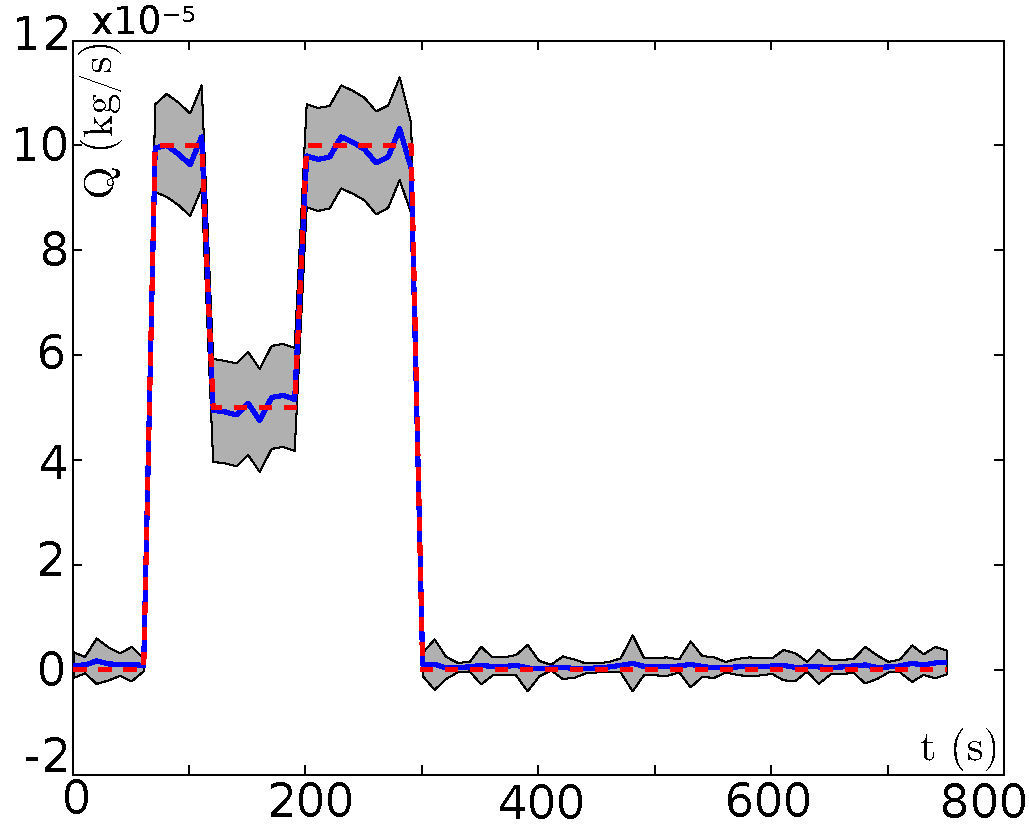
\includegraphics[width=\textwidth]{res_fft07_simu_q_2}
			\caption*{variable}
		\end{subfigure}
		\hfill
		\begin{subfigure}[b]{0.3\textwidth}
			\centering
			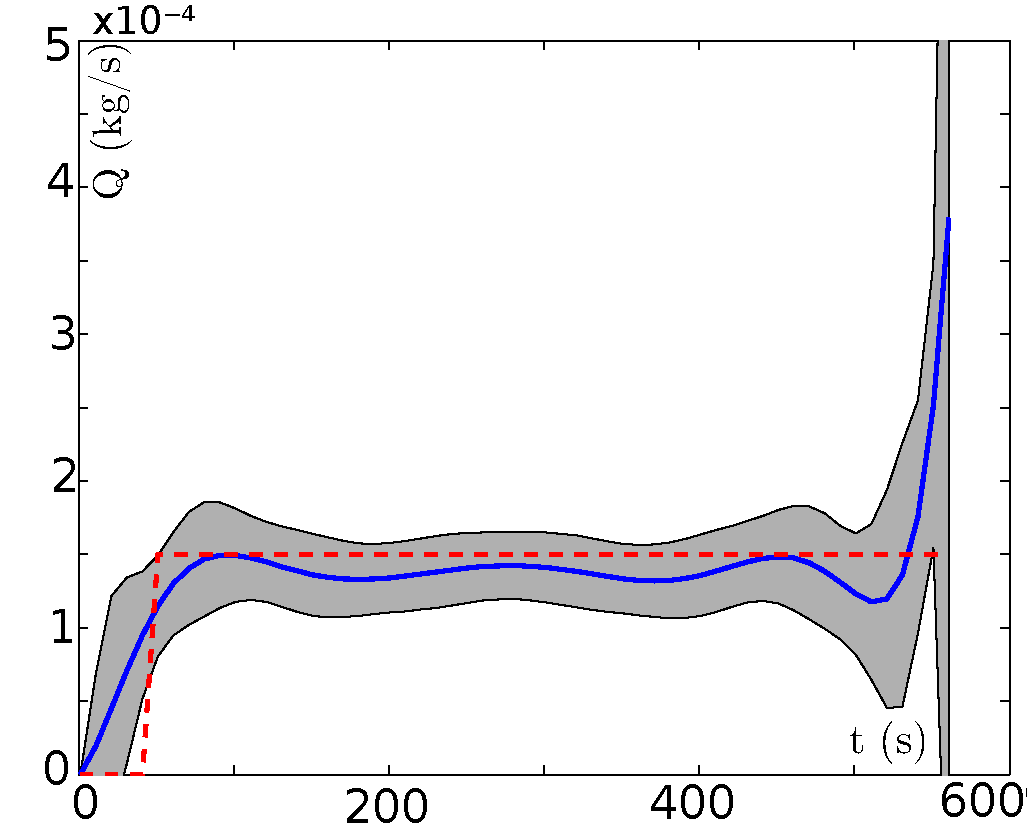
\includegraphics[width=\textwidth]{res_fft07_simu_q_3}
			\caption*{continu}
		\end{subfigure}
	\end{figure}
\end{frame}

%% ======= ==============================================================

\begin{frame}
	\frametitle{Résultats (observations simulées)}
	Comparaison de l'AMIS avec un algorithme MCMC : 
			\begin{figure}
				\centering
				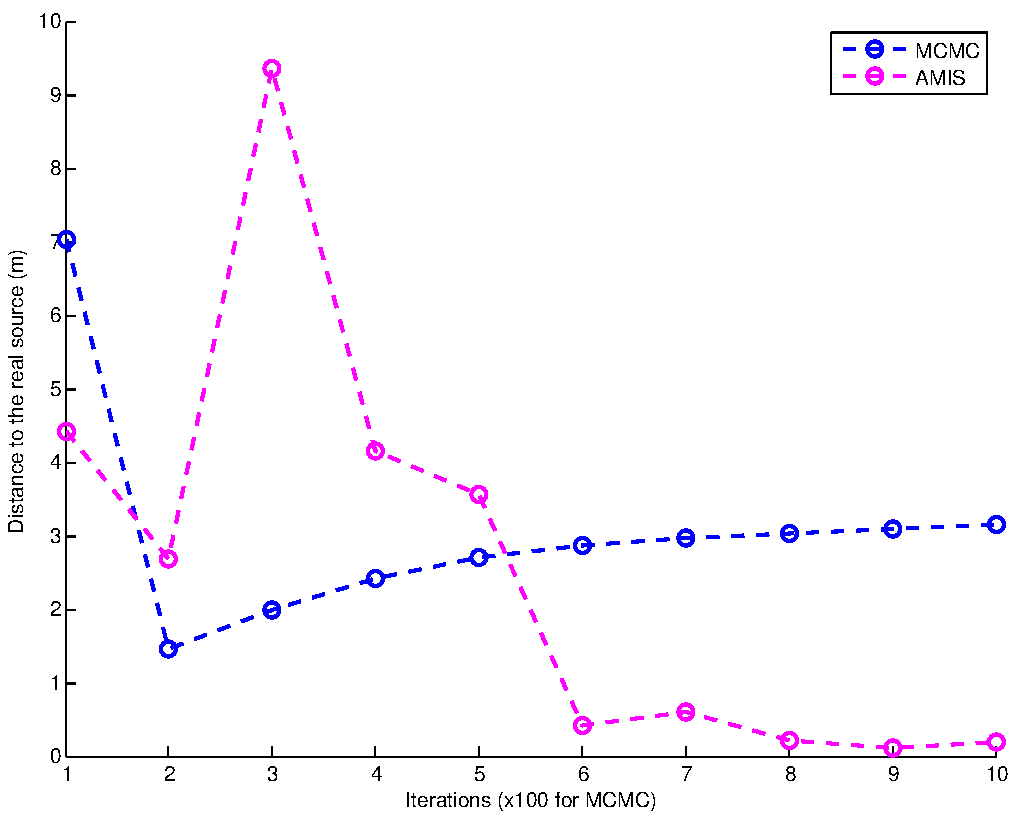
\includegraphics[width=0.65\linewidth]{res_fft07_simu_mcmc}
			\end{figure}
					\centering
{\begin{tabular}{c|ccc}

				&  $\bar{d}(\widehat{\VecPosSource}, \bm{x}_{s^T}) $ & $\sigma_{\widehat{x_s}}$ (m) & $\sigma_{\widehat{y_s}}$ (m)  \\ 
				\hline
				AMIS & $\leq 1$ & $0.9$ & $3.2$ \\
				MCMC & $22.7$ & $130$ & $95$
			\end{tabular}}


\end{frame}

% ==============================================================

\begin{frame}
	\frametitle{Résultats (observations réelles)}
		Comparaison de l'AMIS avec un algorithme MCMC : 
	\begin{figure}
		\centering
			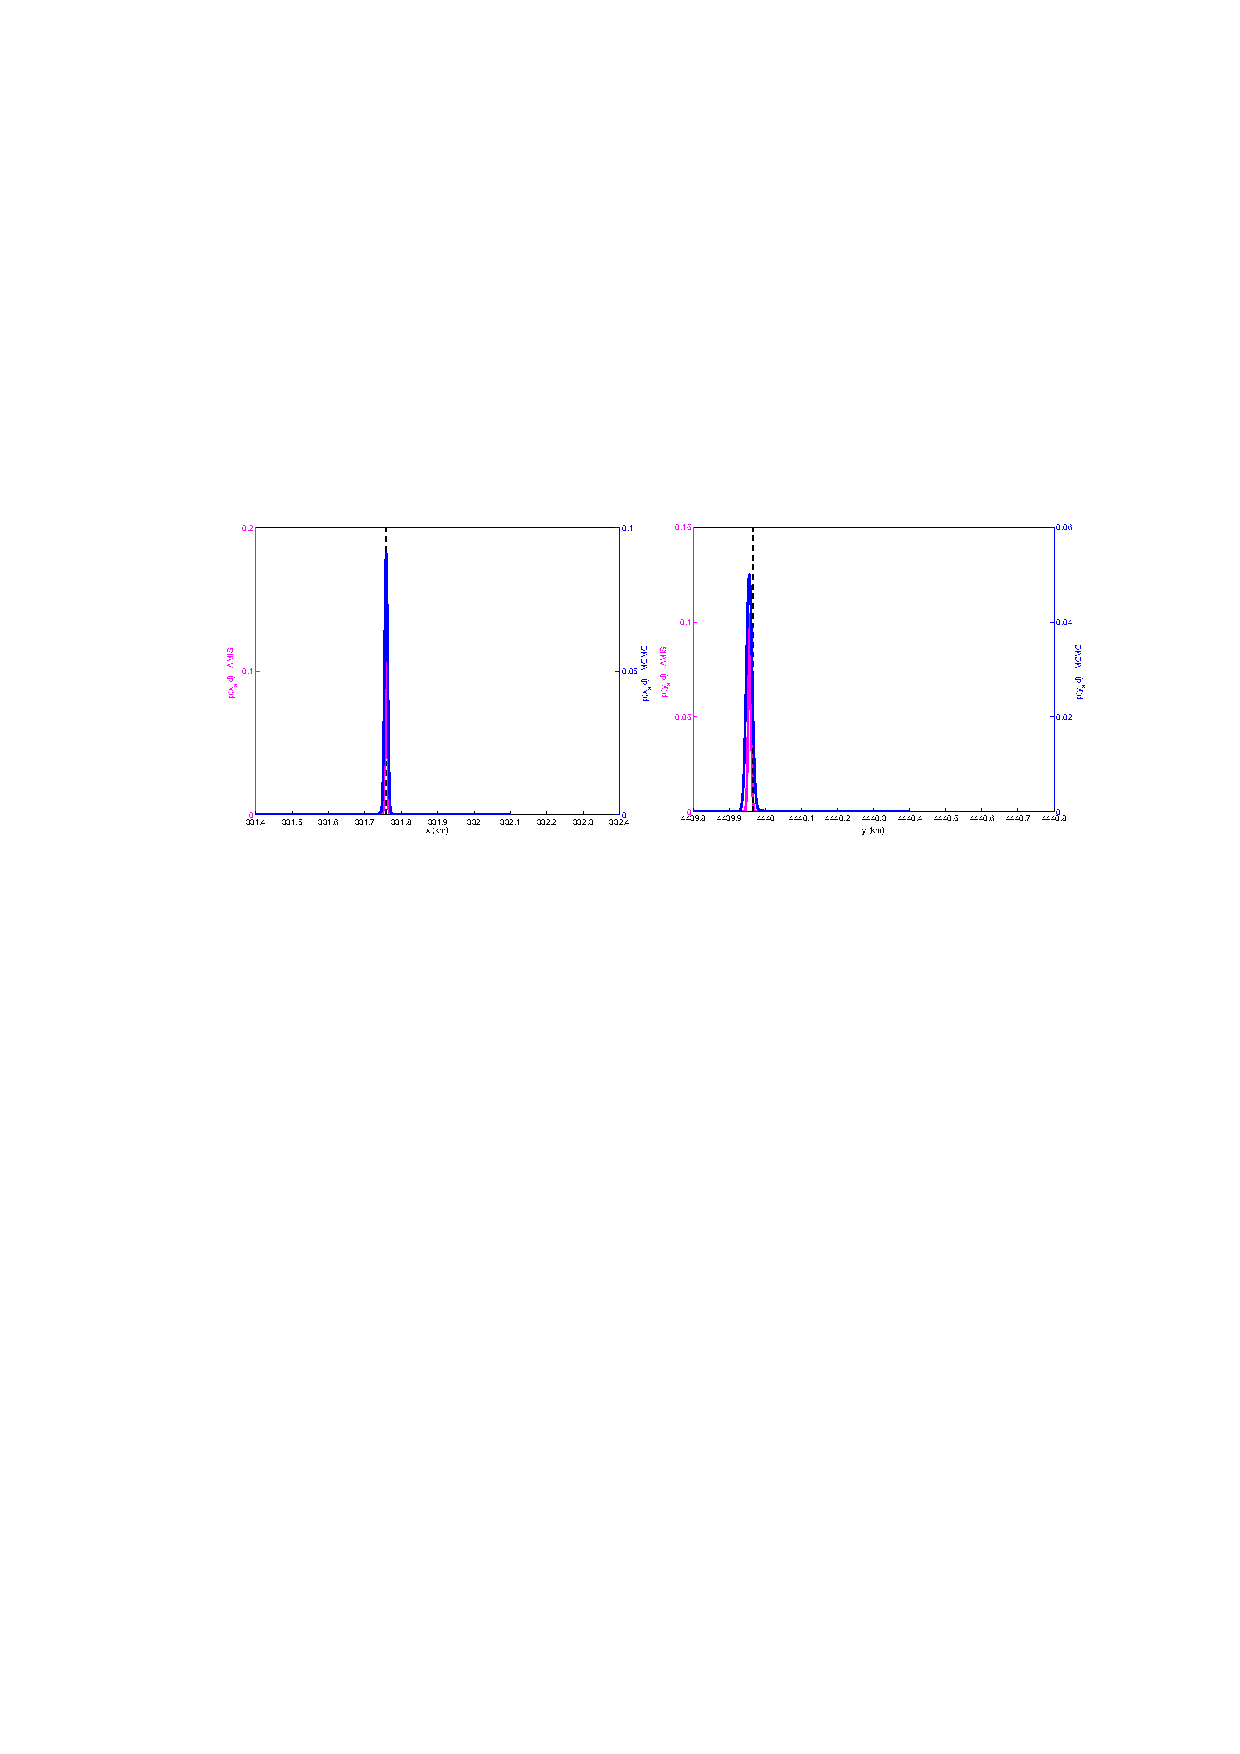
\includegraphics[width=0.8\textwidth]{res_fft07_reel_mcmc} \\
			\vspace{0.6cm}
			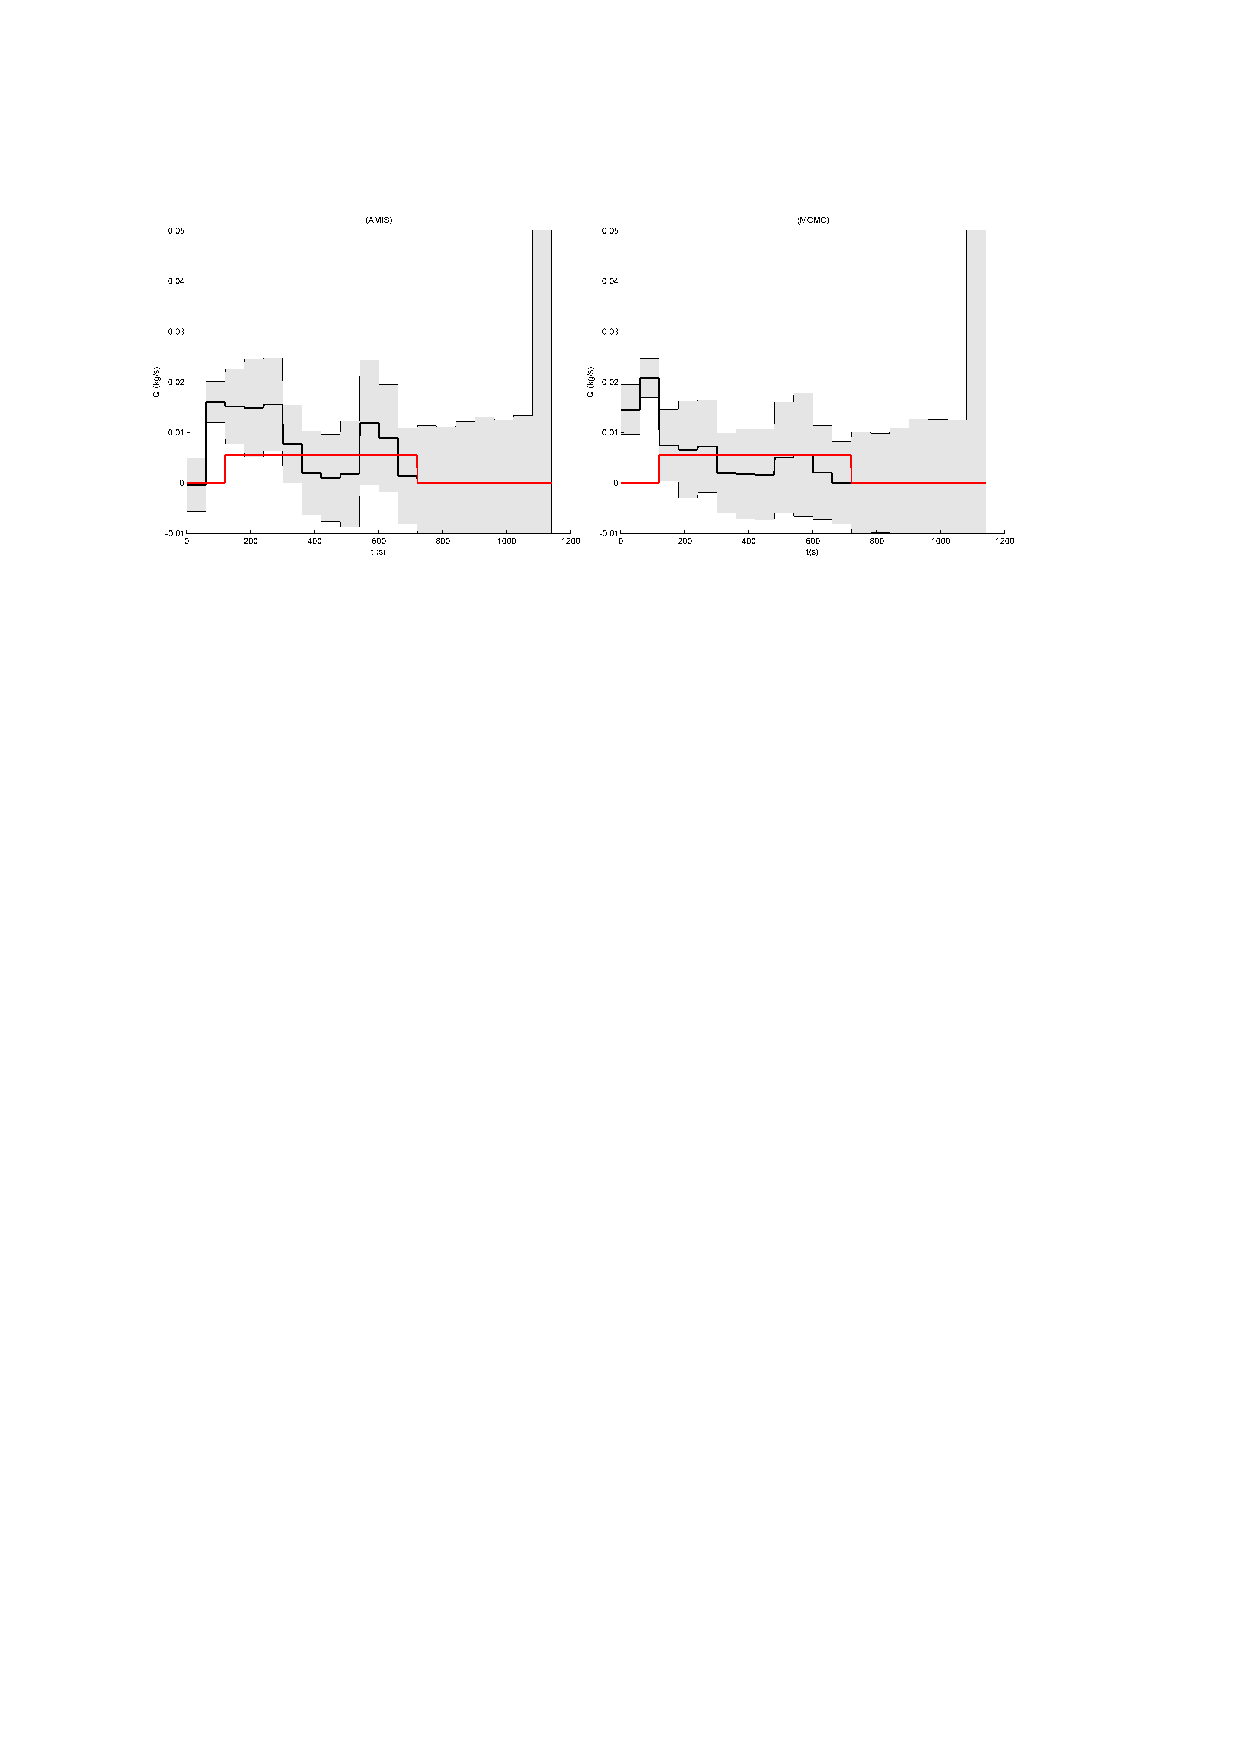
\includegraphics[width = 0.8\textwidth]{res_fft07_reel_q}
	\end{figure}
\end{frame}

% ==============================================================

\begin{frame}
	\frametitle{Cas FFT07: conclusions}
	Résultats publiés dans une revue internationale:
	\begin{important}
		{\small 		\textit{"An adaptive Bayesian inference algorithm to estimate the parameters of a hazardous atmospheric release"} \\ Rajaona et al., Atmospheric Environment, 2015}
	\end{important}
	
	\begin{itemize}
		\item Bons résultats pour la localisation (simulé + réel)
		\item Bonne estimation du profil d'émission (simulé)
		\item Avantages par rapport au MCMC: convergence, précision
		\vspace{0.5cm}
		\item{\color{lightred} résultats approximatifs pour $\widehat{\VecQSource}$ sur données réelles}
		\item charge de calcul concentrée sur la construction des $\MatC(\VecPosSource)$ \\ $\Rightarrow$ {\color{lightred}méthode coûteuse pour modèles plus complexes !}
	\end{itemize}
\end{frame}

% ================================================================

\section{Application avec modèle rétrograde aux cas simulés Beaune et Opéra}

% ================================================================

\begin{frame}
	\frametitle{Nouveaux objectifs}
	
	\begin{itemize}
		\item Passer d'un contexte simple (terrain plat, météo stationnaire) à un environnement plus \textbf{complexe} (relief, bâtiments, météo instationnaire) \\
		$\Rightarrow$ utiliser un \textbf{nouveau modèle de dispersion adapté à cette complexité}
		\item Tester et valider la méthodologie sur des nouveaux cas-tests plus complexes 
	\end{itemize}

\end{frame}

% =================================================================

\begin{frame}
	\frametitle{Modélisation lagrangienne avec PMSS}
	\begin{blueblock}{Dispersion lagrangienne}
		Panache $\Rightarrow$ ensemble de "particules" porteuses d'une masse élémentaire de polluant
	\end{blueblock}
	
	L'outil \textit{Parallel Micro-SWIFT-SPRAY} (PMSS) permet de:
	\begin{columns}
		\column[]{0.5\linewidth}
{\small 			\begin{itemize}
				\item simuler un champ de vent 3D (interpolation + conservation de masse):
			\end{itemize}}
			\begin{figure}
				\centering
				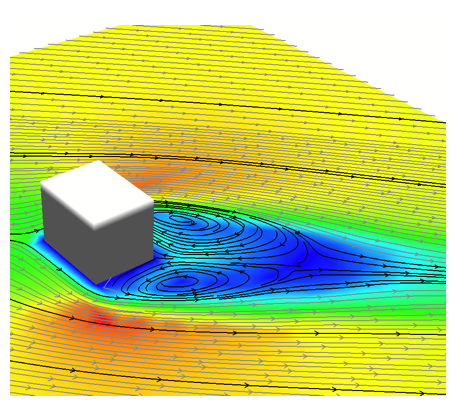
\includegraphics[width=0.45\textwidth]{swift_exemple}
%				\caption*{{\footnotesize SWIFT}}
			\end{figure}
		\column[]{0.5\linewidth}
{\small 			\begin{itemize}
				\item calculer des champs de concentration:
			\end{itemize}}
			\begin{figure}
				\centering
				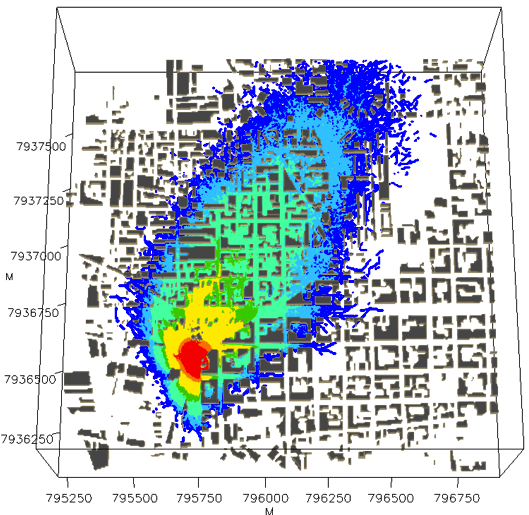
\includegraphics[width=0.45\textwidth]{spray_exemple}
%				\caption*{{\footnotesize SPRAY}}
			\end{figure}
	\end{columns}
	\vspace{0.07cm}
	
{\small 	\begin{itemize}
		\item modélisation de phénomènes complexes
		\item bon ratio performances/temps de calcul
	\end{itemize}}
\end{frame}

% ===============================================================

\begin{frame}
	\frametitle{Couplage PMSS - estimation source}

	Impossible d'utiliser la méthodologie actuelle:
	\begin{itemize}
		\item $KN_p$ appels au modèle pour $K$ itérations et $N_p$ particules AMIS par itération \\ $\Rightarrow$ {\color{lightred}temps de calcul excessif} avec PMSS !
		\item solution: diminuer $N_p$ ? \\
		$\Rightarrow$ {\color{lightred}exploration moins efficace} du domaine
	\end{itemize}
	
	\vspace{1cm}
	
	\textbf{Alternative}: optimiser le mode de calcul des matrices source-récepteur
\end{frame}

% ================================================================

\begin{frame}
%	On découple la construction des matrices source-récepteur de la boucle itérative principale de l'AMIS. Comme ça, la vraisemblance se calcule directement, sans appel au modèle de dispersion.
	\frametitle{Couplage PMSS - estimation source}
	\begin{greenblock}{Solution proposée}
		Pré-calcul des matrices $\MatC(\bm{x})$ en tout point $\bm{x}$ du domaine maillé, avec un modèle de dispersion rétrograde.
	\end{greenblock}
	
	\onslide<1>{Première approche:\\}
	\onslide<2>{Approche optimisée avec pré-calcul:}
	\begin{figure}
		\centering
		\only<1>{
			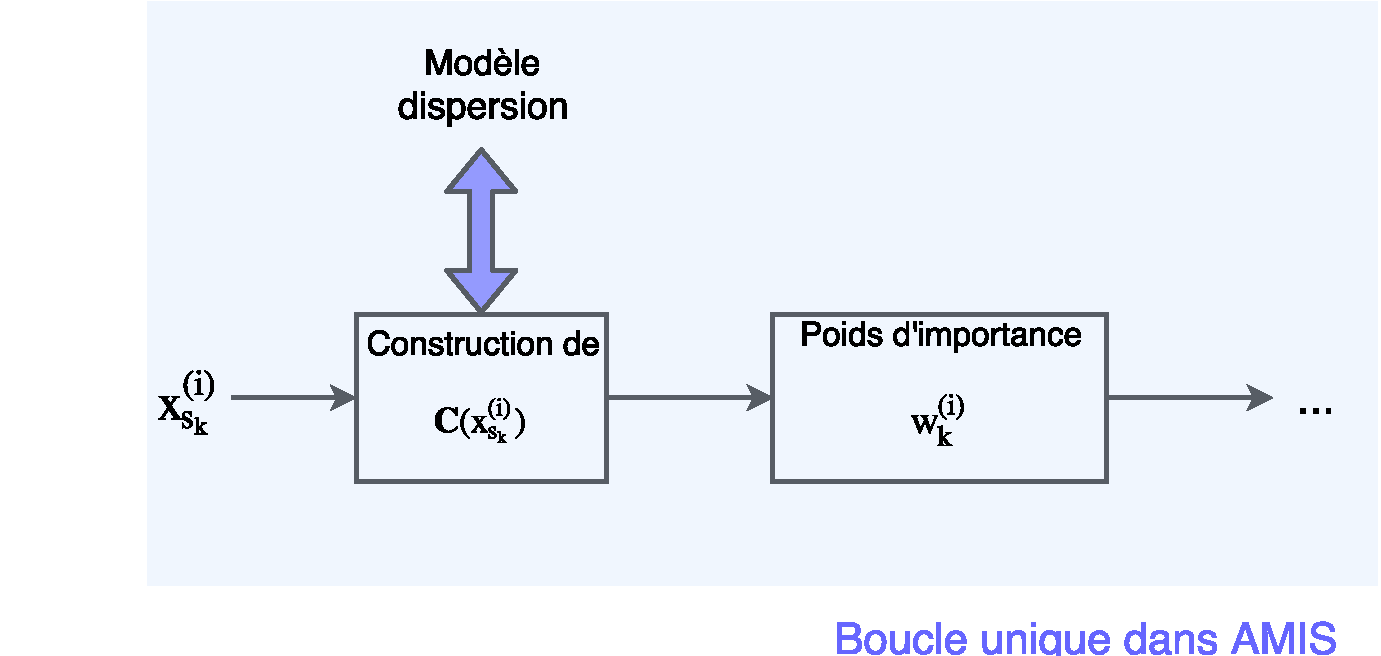
\includegraphics[width=0.9\textwidth]{retrograde_workflow_step_1}
		}
		\only<2>{
			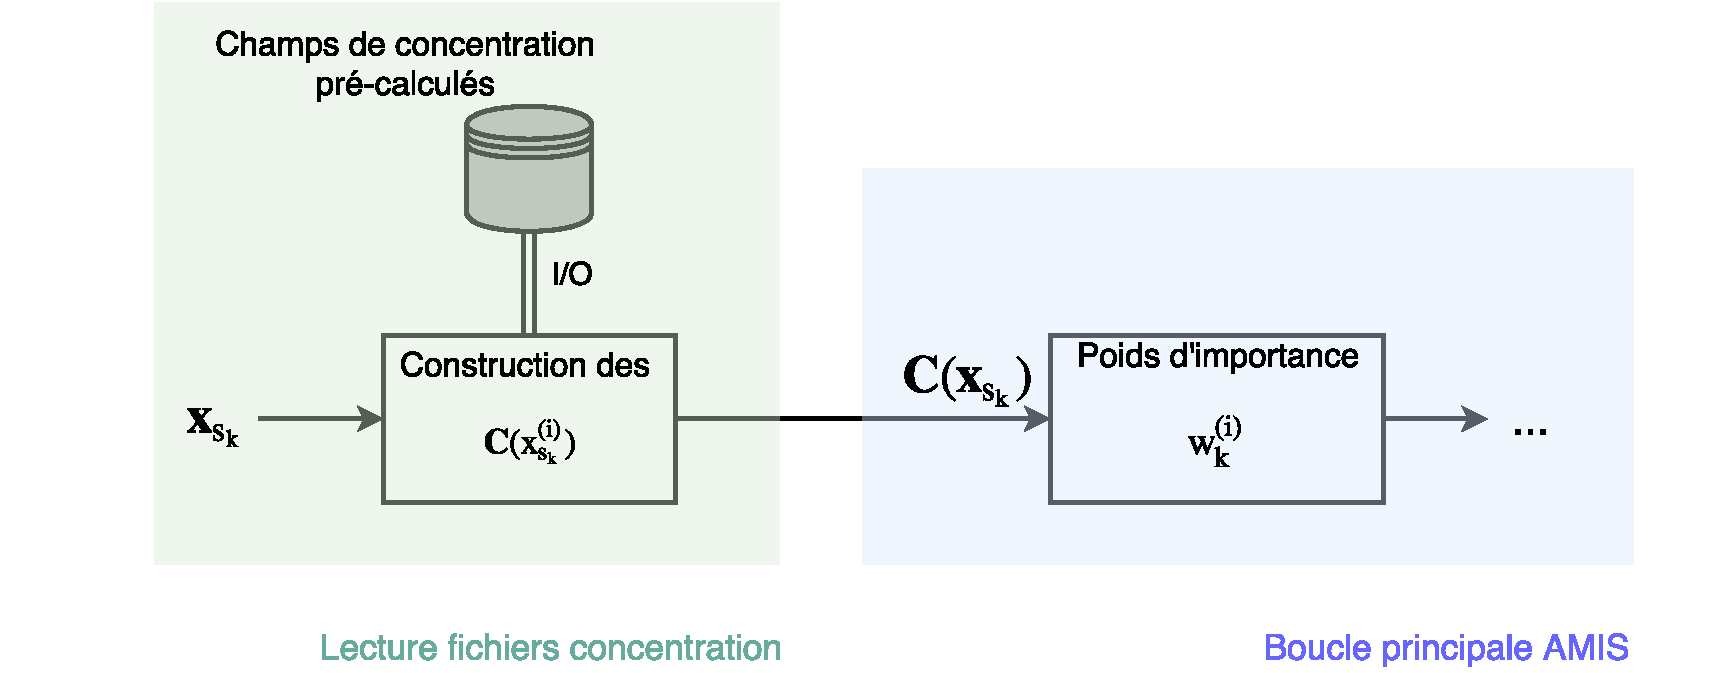
\includegraphics[width=0.9\textwidth]{retrograde_workflow_step_2}
		}
	\end{figure}
\end{frame}

% ==================================================================

\begin{frame}
	\frametitle{Couplage PMSS -estimation source}
	\begin{blueblock}{	Modèle de dispersion rétrograde}
		Permet de construire un champ de rétro-concentrations $C^*$  en "inversant" le processus de dispersion:
		\begin{itemize}
			\item source $\rightarrow$ rétro-capteur
			\item capteurs $\rightarrow$ rétro-sources
			\item inversion du temps et de la direction du vent
		\end{itemize}
	\end{blueblock}
	
	\begin{figure}
		\centering
		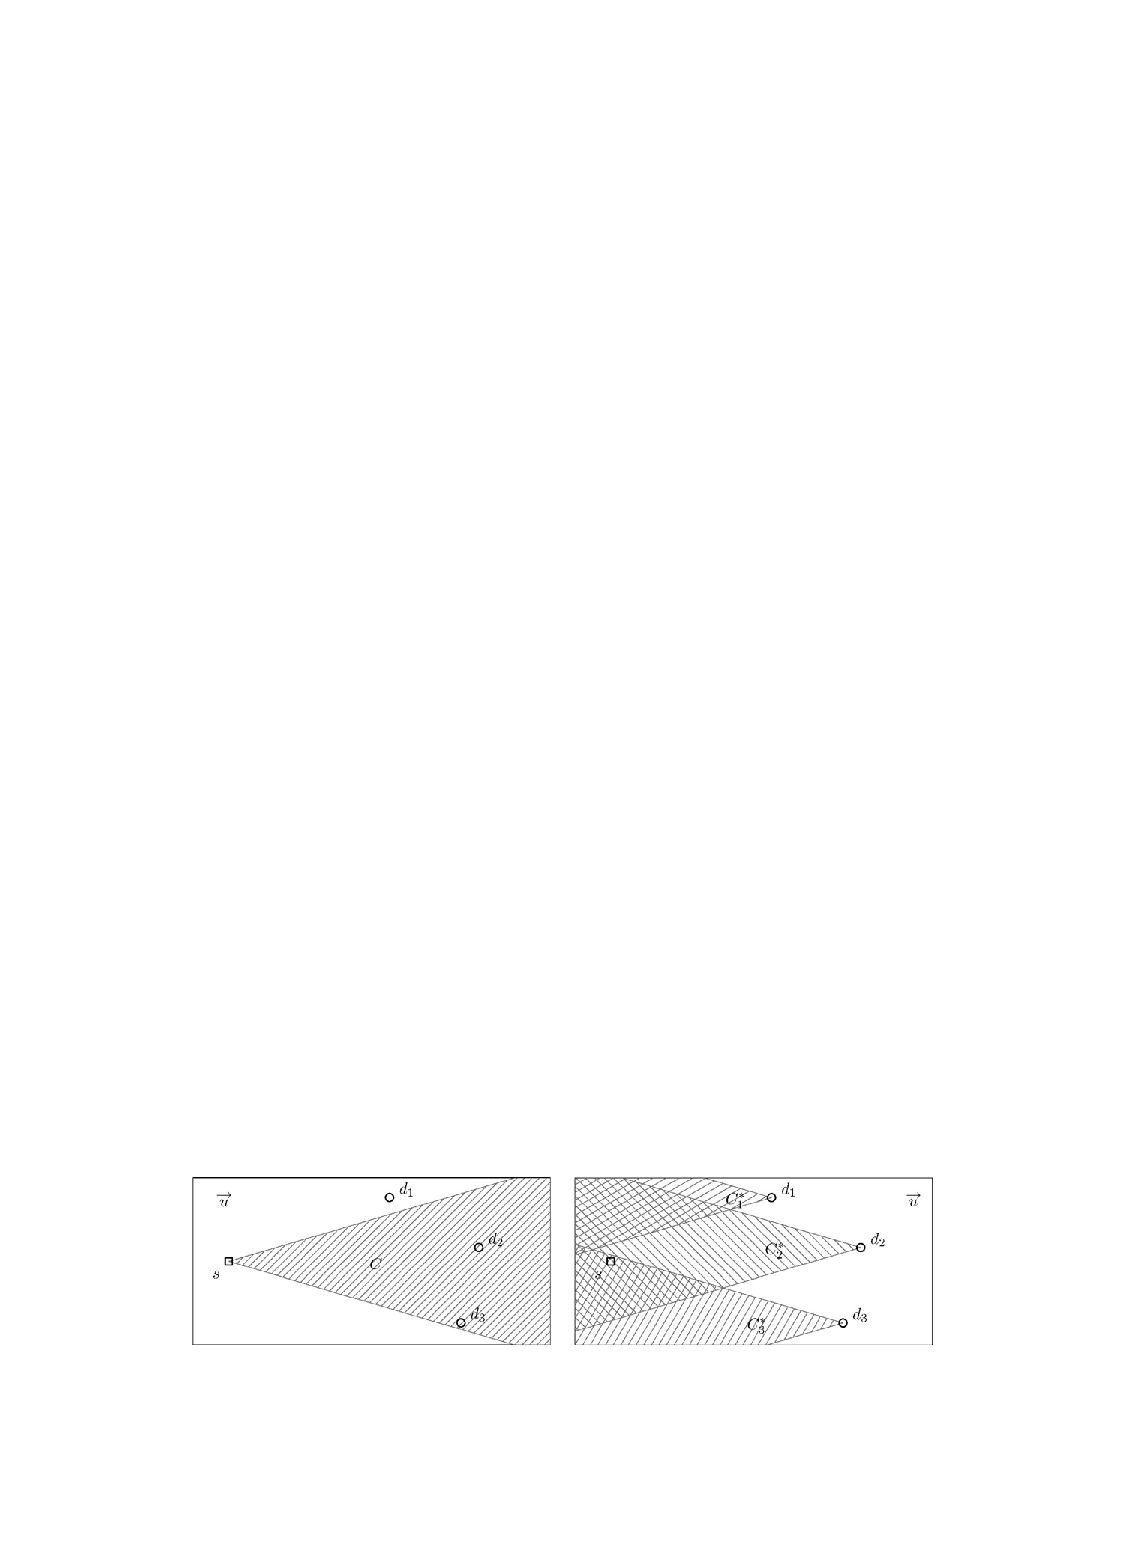
\includegraphics[width=0.8\textwidth]{dualite_direct_inverse}
		\caption*{[Keats et al., 2007]}
	\end{figure}


\end{frame}

% ===========================================================

\begin{frame}
	\frametitle{Couplage PMSS - estimation source}
	
	\begin{blueblock}{Dualité direct-rétrograde}
		Pour un rejet localisé et instantané $(\VecPosSource, t_s)$ on a, au capteur $\bm{x}_{R_i}$ et à l'instant $t_{R_i}$:
		$$ C(\bm{x}_{R_i}, t_{R_i}) = C^* (\VecPosSource, t_s) $$
	\end{blueblock}
	
	
	
	Avantages:
	\begin{itemize}
		\item modèle rétrograde directement intégré à PMSS (RetroSPRAY)
		\item un seul calcul rétrograde par capteur
		\item pré-calcul entièrement parallélisable
		\item suppression des appels au modèle de dispersion pendant les itérations de l'AMIS

	\end{itemize}
\end{frame}

% ==========================================================

\begin{frame}
	\frametitle{Cas simulé Beaune}
	\textbf{Objectif}: valider l'approche avec modèle rétrograde sur un cas de synthèse en milieu rural (relief vallonné):
	\begin{columns}
		\column[]{0.5\linewidth}
{\small 		\begin{itemize}
			\item domaine: 6km $\times$ 6km
			\item vent constant (330$\degree$, 1.5 m/s)
			\item rejet long (45mn)
			\item $N_C$ = 25 capteurs
		\end{itemize}}
		\column[]{0.5\linewidth}
			\animategraphics[autoplay,loop,every=2,type=png,width=1\textwidth]{5}{beaune-}{0}{23}


	\end{columns}
	
\end{frame}

% ============================================================

\begin{frame}
	\frametitle{Cas simulé Beaune: résultats}
	Estimation de la position et du profil d'émission:
	\begin{figure}
		\centering
				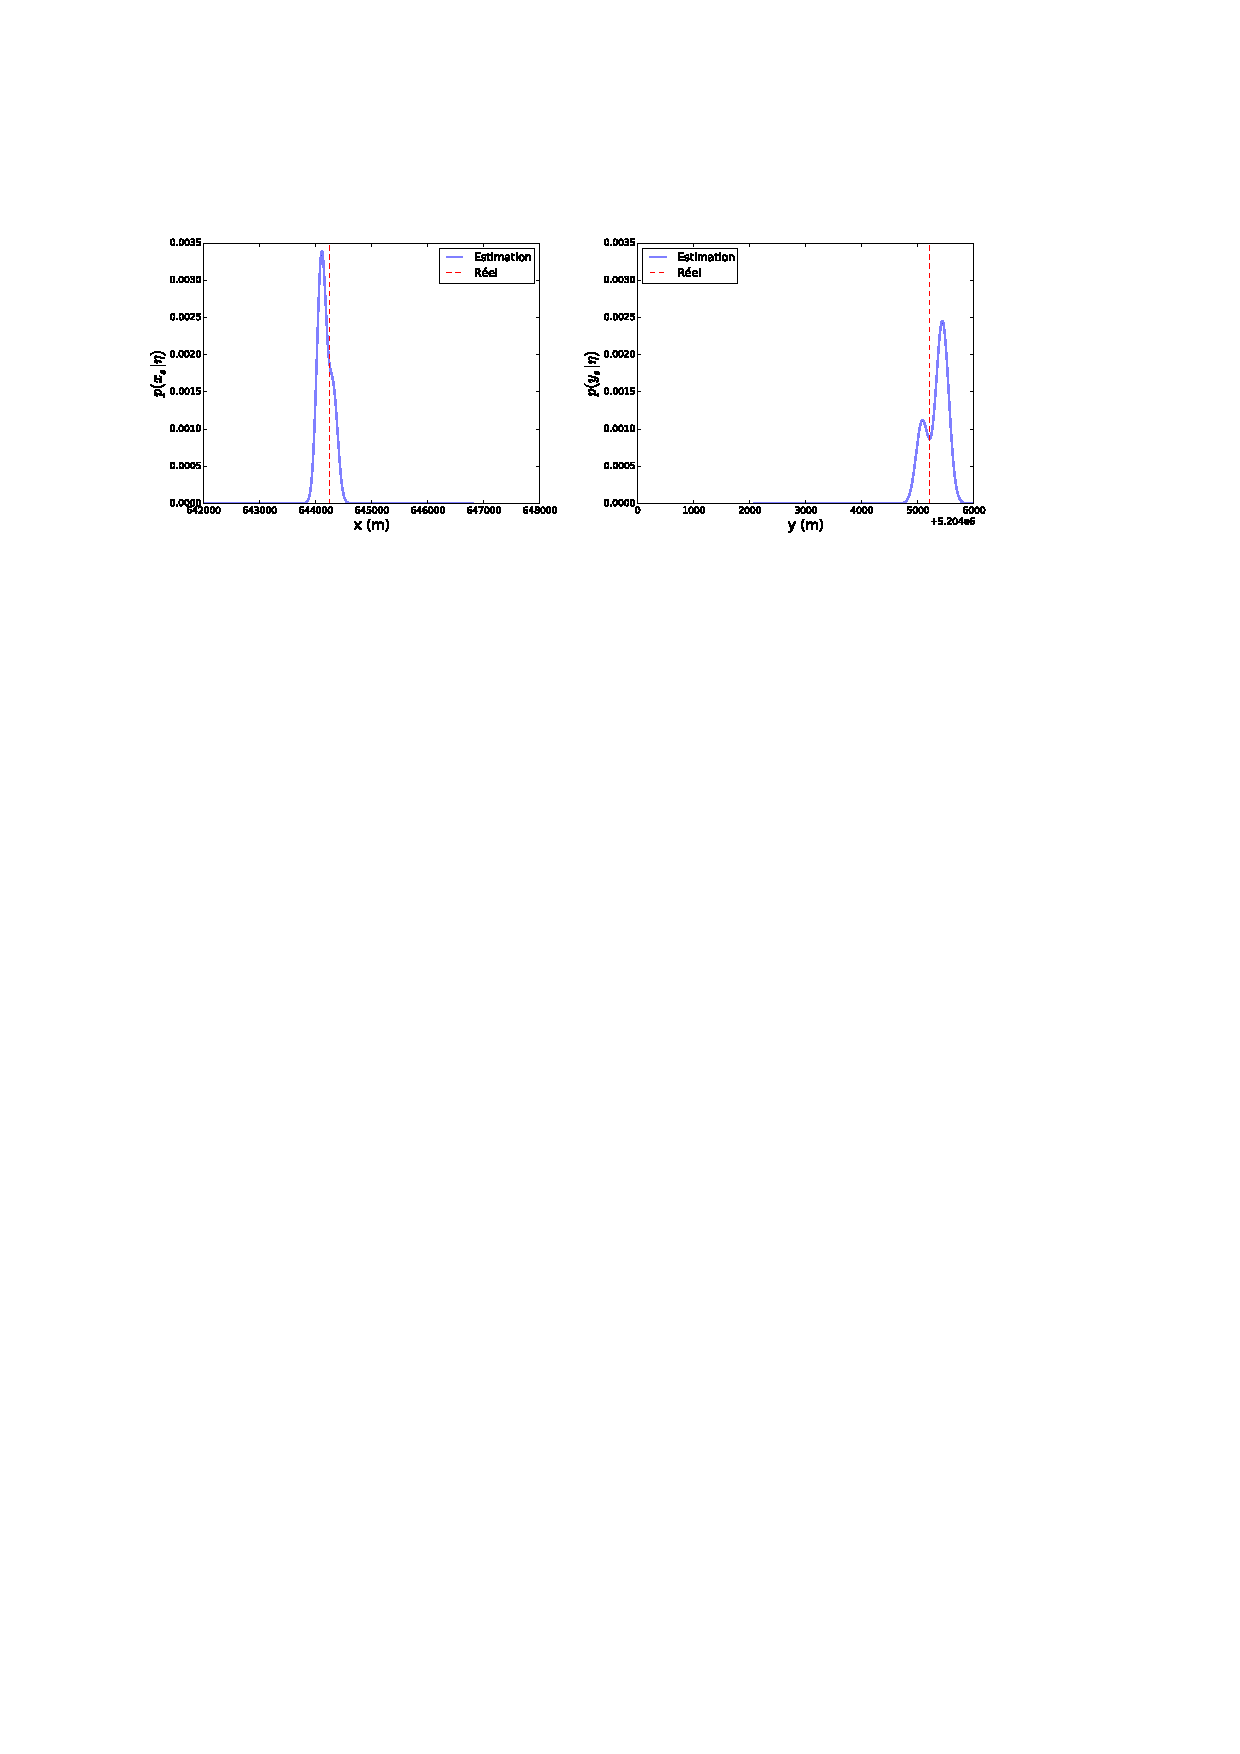
\includegraphics[width=\textwidth]{beaune-position} \\
				\includegraphics[width=0.45\textwidth]{beaune-q}
	\end{figure}
\end{frame}

% ==============================================================
%
%\begin{frame}
%	\frametitle{Cas simulé Beaune: résultats}
%	\only<1>{Influence de la variance d'observation: $\sigma_{obs}^2 = 10^{-7}$}
%	\only<2>{Influence de la variance d'observation: $\sigma_{obs}^2 = 5 \times 10^{-7}$}
%	\only<3>{Influence de la variance d'observation: $\sigma_{obs}^2 = 10^{-6}$}
%	\only<4>{Influence de la variance d'observation: $\sigma_{obs}^2 = 5 \times 10^{-6}$}
%	\only<5>{Influence de la variance d'observation: $\sigma_{obs}^2 = 10^{-5}$}
%	\only<6>{Influence de la variance d'observation: $\sigma_{obs}^2 = 5 \times 10^{-5}$}
%	\begin{columns}
%		\column[]{0.5\linewidth}
%			\begin{figure}
%				\centering
%				\only<1>{\includegraphics[width=0.9\textwidth]{beaune_varobs_1_x}}
%				\only<2>{\includegraphics[width=0.9\textwidth]{beaune_varobs_2_x}}
%				\only<3>{\includegraphics[width=0.9\textwidth]{beaune_varobs_3_x}}
%				\only<4>{\includegraphics[width=0.9\textwidth]{beaune_varobs_4_x}}
%				\only<5>{\includegraphics[width=0.9\textwidth]{beaune_varobs_5_x}}
%				\only<6>{\includegraphics[width=0.9\textwidth]{beaune_varobs_6_x}}
%				\end{figure}
%			\column[]{0.5\linewidth}
%			\begin{figure}
%				\centering
%				\only<1>{\includegraphics[width=0.9\textwidth]{beaune_varobs_1_y}}
%				\only<2>{\includegraphics[width=0.9\textwidth]{beaune_varobs_2_y}}
%				\only<3>{\includegraphics[width=0.9\textwidth]{beaune_varobs_3_y}}
%				\only<4>{\includegraphics[width=0.9\textwidth]{beaune_varobs_4_y}}
%				\only<5>{\includegraphics[width=0.9\textwidth]{beaune_varobs_5_y}}
%				\only<6>{\includegraphics[width=0.9\textwidth]{beaune_varobs_6_y}}
%			\end{figure}
%	\end{columns}
%	\begin{figure}
%			\centering
%			\only<1>{\includegraphics[width=0.45\textwidth]{beaune_varobs_1_q}}
%			\only<2>{\includegraphics[width=0.45\textwidth]{beaune_varobs_2_q}}
%			\only<3>{\includegraphics[width=0.45\textwidth]{beaune_varobs_3_q}}
%			\only<4>{\includegraphics[width=0.45\textwidth]{beaune_varobs_4_q}}
%			\only<5>{\includegraphics[width=0.5\textwidth]{beaune_varobs_5_q}}
%			\only<6>{\includegraphics[width=0.5\textwidth]{beaune_varobs_6_q}}
%		\end{figure}
%
%\end{frame}
% ===========================================================

\begin{frame}
	\frametitle{Cas simulé Beaune: résultats}
	Influence de $\sigma_{obs}^2$:
	\begin{figure}
		\centering
		\includegraphics[width=0.6\textwidth]{beaune_varobs_errors}
	\end{figure}
	
	\begin{itemize}
		\item "confiance" accordée aux observations $\VecObs$
		\item observations simulées \\ $\Rightarrow$  erreur faible pour $\sigma_{obs}^2$ faible
	\end{itemize}
\end{frame}

% =============================================================

\begin{frame}
	\frametitle{Cas simulé Beaune: résultats}
	Influence de $\MatSigma_q = \sigma_q^2 \MatI$:
	\begin{columns}
		\column[]{0.5\textwidth}
			\begin{figure}
				\centering
				\includegraphics[width=0.9\textwidth]{beaune_varq_errors_x}\\
				\includegraphics[width=0.9\textwidth]{beaune_varq_errors_y}
			\end{figure}
%			\begin{itemize}
%				\item localisation variant sur l'axe du vent
%			\end{itemize}
		\column[]{0.5\textwidth}
			\begin{figure}
				\centering
				\includegraphics[width=0.9\textwidth]{beaune_varq_errors_q}
			\end{figure}
			\begin{itemize}
				\item localisation variant sur l'axe du vent
				\item $\sigma_q^2$ trop faible $\Rightarrow$ débit sous-estimé
				\item $\sigma_q^2$ trop élevé $\Rightarrow$ débit surestimé
			\end{itemize}
	\end{columns}
\end{frame}

% ==============================================================

\begin{frame}
	\frametitle{Cas simulé Beaune: résultats}
	Influence du réseau de mesure:
	\begin{itemize}
		\item suppression du capteur le plus informatif
	\end{itemize}
	\begin{figure}
		\centering
		\includegraphics[width=\textwidth]{beaune_reseau_sansR8_position} \\
		\includegraphics[width=0.45\textwidth]{beaune_reseau_sansR8_q}
	\end{figure}
\end{frame}

% ===============================================================

\begin{frame}
	\frametitle{Cas simulé Beaune: résultats}
	Influence du réseau de mesure:
	\begin{itemize}
		\item passage de 25 à 9 capteurs
	\end{itemize}
	\only<1>{
		\begin{figure}
			\centering
			\includegraphics[width=0.45\textwidth]{reseau_25C}
			\includegraphics[width=0.45\textwidth]{reseau_9C}
		\end{figure}
		}
	\only<2>{
		\begin{figure}
			\centering
			\includegraphics[width=0.45\textwidth]{beaune_reseau_9C_x}
			\includegraphics[width=0.45\textwidth]{beaune_reseau_9C_y}
		\end{figure}
		\begin{figure}
			\centering
			\begin{subfigure}[b]{0.33\textwidth}
				\centering
				\includegraphics[width=\textwidth]{beaune_reseau_q1}
			\end{subfigure}
			\hfill
			\begin{subfigure}[b]{0.3\textwidth}
				\centering
				\includegraphics[width=\textwidth]{beaune_reseau_q2}
			\end{subfigure}
			\hfill
			\begin{subfigure}[b]{0.3\textwidth}
				\centering
				\includegraphics[width=\textwidth]{beaune_reseau_q3}
			\end{subfigure}
		\end{figure}
		}
\end{frame}

% ==============================================================

\begin{frame}
	\frametitle{Cas simulé Opéra}
	\textbf{Objectif}: valider l'approche avec modèle rétrograde sur un cas difficile (urbain avec météo instationnaire)
	\begin{columns}
		\column[]{0.5\linewidth}
		{\small 		\begin{itemize}
				\item domaine: 808m $\times$ 882m
				\item bascule de vent:
				\begin{itemize}
					\item 230$\degree$ $\rightarrow$ 180$\degree$ $\rightarrow$ 45$\degree$
					\item vitesse constante (3 m/s)
					\end{itemize}
				\item rejet court (10mn)
				\item $N_C$ = 10 capteurs
			\end{itemize}}
			\column[]{0.5\linewidth}
				\animategraphics[autoplay,loop,every=2,type=png,width=1\textwidth]{5}{opera-}{0}{17}
			
		\end{columns}
			\textbf{Problème}: complexité du cas d'étude \\ $\Rightarrow$ {\color{lightred}convergence impossible} avec une initialisation uniforme !
\end{frame}

% ================================================================

\begin{frame}
	\frametitle{Cas simulé Opéra}

	
	\begin{greenblock}{Initialisation améliorée de la loi de proposition (1/2)}
		\begin{enumerate}
			\item Utiliser le modèle rétrograde pour pondérer chaque point $(x_i, y_j)$ par une "probabilité de présence" $\widetilde{\omega}_{x_i, y_j}^{t_l}$, $~ 1\leq t_l \leq T_s$
			\item Définir la distribution: 
			$$p(\VecTheta | t_l, \VecObs) = \sum\limits_{i=1}^{N_x}\sum\limits_{j=1}^{N_y} \widetilde{\omega}_{x_i, y_j}^{t_l} \mathcal{U}_{[x_{i-1}, x_{i}] \times [y_{j-1},y_j]}(\VecTheta)$$
			
			\begin{figure}
				\centering
				\includegraphics[width=0.4\linewidth]{opera_carte_fitting}
%				\caption*{$p(\VecTheta | t_l, \VecObs) $}
			\end{figure}
		\end{enumerate}
	\end{greenblock}
\end{frame}
	
% ================================================================
\begin{frame}
	\frametitle{Cas simulé Opéra}
	\begin{greenblock}{Initialisation améliorée de la loi de proposition (2/2)}
		\begin{enumerate}
			\setcounter{enumi}{4}
			\item Adapter un mélange de noyaux gaussiens $\psi_{\alpha, \nu}$ à $p(\VecTheta | t_l, \VecObs) $ en minimisant la divergence  $D_{KL}(p(\VecTheta | t_l, \VecObs) || \psi_{\alpha, \nu})$.
			 \begin{figure}
			 	\centering
			 	\includegraphics[width=0.45\linewidth]{opera_resultat_fitting}
			 \end{figure}
			\item Utiliser les paramètres adaptés de $\psi_{\alpha, \nu}$ pour initialiser $\varphi_{\alpha, \nu}$ dans l'algorithme AMIS.
		\end{enumerate}
\end{greenblock}
\end{frame}




% ==================================================================

\begin{frame}
	\frametitle{Cas simulé Opéra: résultats}
Avec initialisation améliorée:
	\begin{figure}
		\centering
		\includegraphics[width=\textwidth]{opera_resultats_position} \\
		\includegraphics[width=0.45\textwidth]{opera_resultats_q}
	\end{figure}
\end{frame}

% ==================================================================

\begin{frame}
	\frametitle{Cas simulés Beaune et Opéra: conclusions}
	Résultats publiés dans une conférence internationale:
	\begin{important}
{\small 		\textit{"A Bayesian approach of the source term estimate coupling retro-dispersion computations with a Lagrangian particle dispersion model and the Adaptive Multiple Importance Sampling"} \\ Rajaona et al., HARMO17, 2016}
	\end{important}
	
	\begin{itemize}
		\item Amélioration du processus d'estimation: 
		\begin{itemize}
			\item couplage avec un modèle de dispersion réaliste (PMSS)
			\item pré-calcul des $\MatC(\VecPosSource)$ $\Rightarrow$ temps de calcul raisonnable (< 5 minutes)
		\end{itemize}
		\item Cas Beaune:
		\begin{itemize}
			\item bons résultats pour localisation et estimation du débit
			\item influence des hyperparamètres $\sigma_{obs}^2$ et $\sigma_q^2$ \\
			$\Rightarrow$ modèle bayésien hiérarchique?
			\item importance du capteur le plus informatif
		\end{itemize}
		\item Cas Opéra:
		\begin{itemize}
			\item bons résultats avec l'initialisation optimisée de l'AMIS
			\item optimisation du tirage des particules AMIS avec présence de bâtiments?
		\end{itemize}
	\end{itemize}
\end{frame}

% ===============================================================
\section{Conclusion et perspectives}
% ===============================================================
\begin{frame}
	\frametitle{Conclusion et perspectives}
	\textbf{Résultats}:
	\begin{itemize}
		\item Méthode permettant une \textbf{estimation simultanée} de la \textbf{localisation} et du \textbf{profil temporel d'émission} d'un rejet atmosphérique
		\item \textbf{Validation} sur des cas-tests synthétiques et expérimentaux 
		\item Couplage de la méthode avec un \textbf{modèle de dispersion complexe} \\
		$\Rightarrow$ {\footnotesize permet d'appréhender des situations difficiles (relief, bâtiments, météo instationnaire) sans ralentir l'algorithme d'estimation}
		\item \textbf{Optimisation de l'initialisation de l'AMIS} avec utilisation d'un modèle rétrograde \\
		$\Rightarrow${\small  illustration de la complémentarité des approches déterministe et probabiliste}
	\end{itemize}
\end{frame}

\begin{frame}
	\frametitle{Conclusion et perspectives}
	
	\textbf{Perspectives}:
	\begin{itemize}
		\item Test et validation sur un cas urbain expérimental:\\
		$\Rightarrow$ {\small Mock Urban Setting (MUST), Joint Urban 2003 ...}
		\item Etude approfondie de l'impact des hyperparamètres
		\item Application au dimensionnement d'un réseau de capteurs:\\
			$\Rightarrow$ {\small recherche de la topologie optimale pour un problème STE}
		\item Traitement séquentiel des observations:\\
			$\Rightarrow$ {\small évaluer une séquence de distributions a posteriori en ré-utilisant l'information des particules existantes (SMC\footnote{\textit{\textbf{S}equential \textbf{M}onte \textbf{C}arlo}} \textit{sampler})}
	\end{itemize}
\end{frame}

% =================================================================

\begin{frame}
	\begin{center}
		Merci pour votre attention !
	\end{center}
\end{frame}
\end{document}
